\documentclass{book}
\usepackage[a4paper,top=2.5cm,bottom=2.5cm,left=2.5cm,right=2.5cm]{geometry}
\usepackage{makeidx}
\usepackage{natbib}
\usepackage{graphicx}
\usepackage{multicol}
\usepackage{float}
\usepackage{listings}
\usepackage{color}
\usepackage{ifthen}
\usepackage[table]{xcolor}
\usepackage{textcomp}
\usepackage{alltt}
\usepackage{ifpdf}
\ifpdf
\usepackage[pdftex,
            pagebackref=true,
            colorlinks=true,
            linkcolor=blue,
            unicode
           ]{hyperref}
\else
\usepackage[ps2pdf,
            pagebackref=true,
            colorlinks=true,
            linkcolor=blue,
            unicode
           ]{hyperref}
\usepackage{pspicture}
\fi
\usepackage[utf8]{inputenc}
\usepackage{mathptmx}
\usepackage[scaled=.90]{helvet}
\usepackage{courier}
\usepackage{sectsty}
\usepackage{amssymb}
\usepackage[titles]{tocloft}
\usepackage{doxygen}
\lstset{language=C++,inputencoding=utf8,basicstyle=\footnotesize,breaklines=true,breakatwhitespace=true,tabsize=4,numbers=left }
\makeindex
\setcounter{tocdepth}{3}
\renewcommand{\footrulewidth}{0.4pt}
\renewcommand{\familydefault}{\sfdefault}
\hfuzz=15pt
\setlength{\emergencystretch}{15pt}
\hbadness=750
\tolerance=750
\begin{document}
\hypersetup{pageanchor=false,citecolor=blue}
\begin{titlepage}
\vspace*{7cm}
\begin{center}
{\Large My Project }\\
\vspace*{1cm}
{\large Generated by Doxygen 1.8.2}\\
\vspace*{0.5cm}
{\small Tue Feb 14 2017 06:21:02}\\
\end{center}
\end{titlepage}
\clearemptydoublepage
\pagenumbering{roman}
\tableofcontents
\clearemptydoublepage
\pagenumbering{arabic}
\hypersetup{pageanchor=true,citecolor=blue}
\chapter{Hierarchical Index}
\section{Class Hierarchy}
This inheritance list is sorted roughly, but not completely, alphabetically\-:\begin{DoxyCompactList}
\item \contentsline{section}{Piece.\-Implementation.\-Bishop\-Test}{\pageref{classPiece_1_1Implementation_1_1BishopTest}}{}
\item \contentsline{section}{Board.\-Board}{\pageref{classBoard_1_1Board}}{}
\item \contentsline{section}{Board.\-Board\-Test}{\pageref{classBoard_1_1BoardTest}}{}
\item \contentsline{section}{Piece.\-Implementation.\-Custom\-Piece1\-Test}{\pageref{classPiece_1_1Implementation_1_1CustomPiece1Test}}{}
\item \contentsline{section}{Piece.\-Implementation.\-Custom\-Piece2\-Test}{\pageref{classPiece_1_1Implementation_1_1CustomPiece2Test}}{}
\item \contentsline{section}{Util.\-Direction}{\pageref{classUtil_1_1Direction}}{}
\item \contentsline{section}{Util.\-Direction\-Test}{\pageref{classUtil_1_1DirectionTest}}{}
\item \contentsline{section}{Game.\-Game}{\pageref{classGame_1_1Game}}{}
\item \contentsline{section}{Piece.\-Implementation.\-King\-Test}{\pageref{classPiece_1_1Implementation_1_1KingTest}}{}
\item \contentsline{section}{Piece.\-Implementation.\-Knight\-Test}{\pageref{classPiece_1_1Implementation_1_1KnightTest}}{}
\item \contentsline{section}{Piece.\-Implementation.\-Pawn\-Test}{\pageref{classPiece_1_1Implementation_1_1PawnTest}}{}
\item \contentsline{section}{Piece.\-Piece}{\pageref{classPiece_1_1Piece}}{}
\begin{DoxyCompactList}
\item \contentsline{section}{Piece.\-Implementation.\-Bishop}{\pageref{classPiece_1_1Implementation_1_1Bishop}}{}
\item \contentsline{section}{Piece.\-Implementation.\-Custom\-Piece1}{\pageref{classPiece_1_1Implementation_1_1CustomPiece1}}{}
\item \contentsline{section}{Piece.\-Implementation.\-Custom\-Piece2}{\pageref{classPiece_1_1Implementation_1_1CustomPiece2}}{}
\item \contentsline{section}{Piece.\-Implementation.\-King}{\pageref{classPiece_1_1Implementation_1_1King}}{}
\item \contentsline{section}{Piece.\-Implementation.\-Knight}{\pageref{classPiece_1_1Implementation_1_1Knight}}{}
\item \contentsline{section}{Piece.\-Implementation.\-Pawn}{\pageref{classPiece_1_1Implementation_1_1Pawn}}{}
\item \contentsline{section}{Piece.\-Implementation.\-Queen}{\pageref{classPiece_1_1Implementation_1_1Queen}}{}
\item \contentsline{section}{Piece.\-Implementation.\-Rook}{\pageref{classPiece_1_1Implementation_1_1Rook}}{}
\end{DoxyCompactList}
\item \contentsline{section}{Piece.\-Piece\-Type}{\pageref{enumPiece_1_1PieceType}}{}
\item \contentsline{section}{Util.\-Position}{\pageref{classUtil_1_1Position}}{}
\item \contentsline{section}{Util.\-Position\-Test}{\pageref{classUtil_1_1PositionTest}}{}
\item \contentsline{section}{Piece.\-Implementation.\-Queen\-Test}{\pageref{classPiece_1_1Implementation_1_1QueenTest}}{}
\item \contentsline{section}{Piece.\-Implementation.\-Rook\-Test}{\pageref{classPiece_1_1Implementation_1_1RookTest}}{}
\item \contentsline{section}{Game.\-User}{\pageref{classGame_1_1User}}{}
\item \contentsline{section}{User\-Interface.\-User\-Interface}{\pageref{classUserInterface_1_1UserInterface}}{}
\end{DoxyCompactList}

\chapter{Class Index}
\section{Class List}
Here are the classes, structs, unions and interfaces with brief descriptions\-:\begin{DoxyCompactList}
\item\contentsline{section}{\hyperlink{classPiece_1_1Implementation_1_1Bishop}{Piece.\-Implementation.\-Bishop} }{\pageref{classPiece_1_1Implementation_1_1Bishop}}{}
\item\contentsline{section}{\hyperlink{classPiece_1_1Implementation_1_1BishopTest}{Piece.\-Implementation.\-Bishop\-Test} }{\pageref{classPiece_1_1Implementation_1_1BishopTest}}{}
\item\contentsline{section}{\hyperlink{classBoard_1_1Board}{Board.\-Board} }{\pageref{classBoard_1_1Board}}{}
\item\contentsline{section}{\hyperlink{classBoard_1_1BoardTest}{Board.\-Board\-Test} }{\pageref{classBoard_1_1BoardTest}}{}
\item\contentsline{section}{\hyperlink{classPiece_1_1Implementation_1_1CustomPiece1}{Piece.\-Implementation.\-Custom\-Piece1} }{\pageref{classPiece_1_1Implementation_1_1CustomPiece1}}{}
\item\contentsline{section}{\hyperlink{classPiece_1_1Implementation_1_1CustomPiece1Test}{Piece.\-Implementation.\-Custom\-Piece1\-Test} }{\pageref{classPiece_1_1Implementation_1_1CustomPiece1Test}}{}
\item\contentsline{section}{\hyperlink{classPiece_1_1Implementation_1_1CustomPiece2}{Piece.\-Implementation.\-Custom\-Piece2} }{\pageref{classPiece_1_1Implementation_1_1CustomPiece2}}{}
\item\contentsline{section}{\hyperlink{classPiece_1_1Implementation_1_1CustomPiece2Test}{Piece.\-Implementation.\-Custom\-Piece2\-Test} }{\pageref{classPiece_1_1Implementation_1_1CustomPiece2Test}}{}
\item\contentsline{section}{\hyperlink{classUtil_1_1Direction}{Util.\-Direction} }{\pageref{classUtil_1_1Direction}}{}
\item\contentsline{section}{\hyperlink{classUtil_1_1DirectionTest}{Util.\-Direction\-Test} }{\pageref{classUtil_1_1DirectionTest}}{}
\item\contentsline{section}{\hyperlink{classGame_1_1Game}{Game.\-Game} }{\pageref{classGame_1_1Game}}{}
\item\contentsline{section}{\hyperlink{classPiece_1_1Implementation_1_1King}{Piece.\-Implementation.\-King} }{\pageref{classPiece_1_1Implementation_1_1King}}{}
\item\contentsline{section}{\hyperlink{classPiece_1_1Implementation_1_1KingTest}{Piece.\-Implementation.\-King\-Test} }{\pageref{classPiece_1_1Implementation_1_1KingTest}}{}
\item\contentsline{section}{\hyperlink{classPiece_1_1Implementation_1_1Knight}{Piece.\-Implementation.\-Knight} }{\pageref{classPiece_1_1Implementation_1_1Knight}}{}
\item\contentsline{section}{\hyperlink{classPiece_1_1Implementation_1_1KnightTest}{Piece.\-Implementation.\-Knight\-Test} }{\pageref{classPiece_1_1Implementation_1_1KnightTest}}{}
\item\contentsline{section}{\hyperlink{classPiece_1_1Implementation_1_1Pawn}{Piece.\-Implementation.\-Pawn} }{\pageref{classPiece_1_1Implementation_1_1Pawn}}{}
\item\contentsline{section}{\hyperlink{classPiece_1_1Implementation_1_1PawnTest}{Piece.\-Implementation.\-Pawn\-Test} }{\pageref{classPiece_1_1Implementation_1_1PawnTest}}{}
\item\contentsline{section}{\hyperlink{classPiece_1_1Piece}{Piece.\-Piece} }{\pageref{classPiece_1_1Piece}}{}
\item\contentsline{section}{\hyperlink{enumPiece_1_1PieceType}{Piece.\-Piece\-Type} }{\pageref{enumPiece_1_1PieceType}}{}
\item\contentsline{section}{\hyperlink{classUtil_1_1Position}{Util.\-Position} }{\pageref{classUtil_1_1Position}}{}
\item\contentsline{section}{\hyperlink{classUtil_1_1PositionTest}{Util.\-Position\-Test} }{\pageref{classUtil_1_1PositionTest}}{}
\item\contentsline{section}{\hyperlink{classPiece_1_1Implementation_1_1Queen}{Piece.\-Implementation.\-Queen} }{\pageref{classPiece_1_1Implementation_1_1Queen}}{}
\item\contentsline{section}{\hyperlink{classPiece_1_1Implementation_1_1QueenTest}{Piece.\-Implementation.\-Queen\-Test} }{\pageref{classPiece_1_1Implementation_1_1QueenTest}}{}
\item\contentsline{section}{\hyperlink{classPiece_1_1Implementation_1_1Rook}{Piece.\-Implementation.\-Rook} }{\pageref{classPiece_1_1Implementation_1_1Rook}}{}
\item\contentsline{section}{\hyperlink{classPiece_1_1Implementation_1_1RookTest}{Piece.\-Implementation.\-Rook\-Test} }{\pageref{classPiece_1_1Implementation_1_1RookTest}}{}
\item\contentsline{section}{\hyperlink{classGame_1_1User}{Game.\-User} }{\pageref{classGame_1_1User}}{}
\item\contentsline{section}{\hyperlink{classUserInterface_1_1UserInterface}{User\-Interface.\-User\-Interface} }{\pageref{classUserInterface_1_1UserInterface}}{}
\end{DoxyCompactList}

\chapter{Class Documentation}
\hypertarget{classPiece_1_1Implementation_1_1Bishop}{\section{Piece.\-Implementation.\-Bishop Class Reference}
\label{classPiece_1_1Implementation_1_1Bishop}\index{Piece.\-Implementation.\-Bishop@{Piece.\-Implementation.\-Bishop}}
}
Inheritance diagram for Piece.\-Implementation.\-Bishop\-:\begin{figure}[H]
\begin{center}
\leavevmode
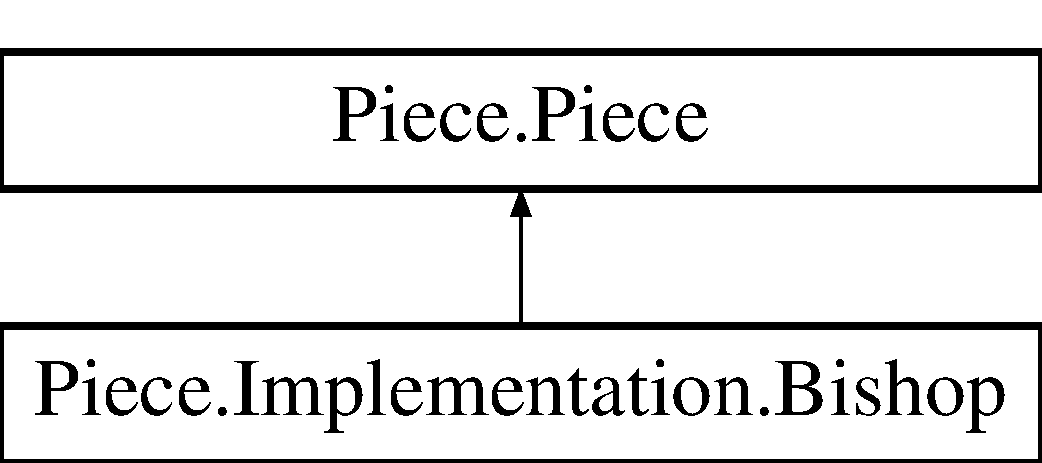
\includegraphics[height=2.000000cm]{classPiece_1_1Implementation_1_1Bishop}
\end{center}
\end{figure}
\subsection*{Public Member Functions}
\begin{DoxyCompactItemize}
\item 
\hyperlink{classPiece_1_1Implementation_1_1Bishop_a94578631257280ceb1491c0d1cd1bb6a}{Bishop} (\hyperlink{classUtil_1_1Position}{Position} start\-Position, int assign\-User\-Id, int assign\-Piece\-Id)  throws Exception 
\item 
\hyperlink{classPiece_1_1Implementation_1_1Bishop_a94578631257280ceb1491c0d1cd1bb6a}{Bishop} (\hyperlink{classUtil_1_1Position}{Position} start\-Position, int assign\-User\-Id, int assign\-Piece\-Id)  throws Exception 
\end{DoxyCompactItemize}

\hypertarget{classPiece_1_1Implementation_1_1BishopTest}{\section{Piece.\-Implementation.\-Bishop\-Test Class Reference}
\label{classPiece_1_1Implementation_1_1BishopTest}\index{Piece.\-Implementation.\-Bishop\-Test@{Piece.\-Implementation.\-Bishop\-Test}}
}
\subsection*{Public Member Functions}
\begin{DoxyCompactItemize}
\item 
void \hyperlink{classPiece_1_1Implementation_1_1BishopTest_afde1aba404e41da9eb303cf2d2975b5f}{set\-Up} ()  throws Exception 
\item 
\hypertarget{classPiece_1_1Implementation_1_1BishopTest_a19d4ab0e8c7d1ef95a20b649017c578d}{void {\bfseries test\-Piece\-Type} ()}\label{classPiece_1_1Implementation_1_1BishopTest_a19d4ab0e8c7d1ef95a20b649017c578d}

\item 
\hypertarget{classPiece_1_1Implementation_1_1BishopTest_ad78bf35582e6089377a8bb6e6974f078}{void {\bfseries test\-Can\-Move} ()  throws Exception}\label{classPiece_1_1Implementation_1_1BishopTest_ad78bf35582e6089377a8bb6e6974f078}

\item 
\hypertarget{classPiece_1_1Implementation_1_1BishopTest_a6e757167fdab7c92e7195aa7ce6c66aa}{void {\bfseries test\-Move} ()  throws Exception}\label{classPiece_1_1Implementation_1_1BishopTest_a6e757167fdab7c92e7195aa7ce6c66aa}

\item 
\hypertarget{classPiece_1_1Implementation_1_1BishopTest_a213353459419a6c78134e5205b3010f7}{void {\bfseries test\-Get\-Functions} ()}\label{classPiece_1_1Implementation_1_1BishopTest_a213353459419a6c78134e5205b3010f7}

\end{DoxyCompactItemize}


\subsection{Detailed Description}
Created by taccio on 2/13/17. 

\subsection{Member Function Documentation}
\hypertarget{classPiece_1_1Implementation_1_1BishopTest_afde1aba404e41da9eb303cf2d2975b5f}{\index{Piece\-::\-Implementation\-::\-Bishop\-Test@{Piece\-::\-Implementation\-::\-Bishop\-Test}!set\-Up@{set\-Up}}
\index{set\-Up@{set\-Up}!Piece::Implementation::BishopTest@{Piece\-::\-Implementation\-::\-Bishop\-Test}}
\subsubsection[{set\-Up}]{\setlength{\rightskip}{0pt plus 5cm}void Piece.\-Implementation.\-Bishop\-Test.\-set\-Up (
\begin{DoxyParamCaption}
{}
\end{DoxyParamCaption}
)  throws Exception \hspace{0.3cm}{\ttfamily [inline]}}}\label{classPiece_1_1Implementation_1_1BishopTest_afde1aba404e41da9eb303cf2d2975b5f}
Calls setup function before every test function 
\begin{DoxyExceptions}{Exceptions}
{\em Exception} & \\
\hline
\end{DoxyExceptions}


The documentation for this class was generated from the following file\-:\begin{DoxyCompactItemize}
\item 
test/\-Piece/\-Implementation/Bishop\-Test.\-java\end{DoxyCompactItemize}

\hypertarget{classBoard_1_1Board}{\section{Board.\-Board Class Reference}
\label{classBoard_1_1Board}\index{Board.\-Board@{Board.\-Board}}
}
\subsection*{Public Member Functions}
\begin{DoxyCompactItemize}
\item 
\hyperlink{classBoard_1_1Board_a652faf97b9270325dfec42e9878dde03}{Board} (\hyperlink{classPiece_1_1Piece}{Piece}\mbox{[}$\,$\mbox{]} pieces, int\mbox{[}$\,$\mbox{]} limit)  throws Exception 
\item 
boolean \hyperlink{classBoard_1_1Board_aca3851cdb777a92a5cf7d2606f08a0b2}{is\-Out\-Of\-Bound} (\hyperlink{classUtil_1_1Position}{Position} target\-Position)
\item 
boolean \hyperlink{classBoard_1_1Board_aa3a97aabcffb32d0c8d93770002af58a}{is\-Out\-Of\-Bound} (int x, int y)
\item 
\hyperlink{classPiece_1_1Piece}{Piece} \hyperlink{classBoard_1_1Board_a86de1febbcfdc2ea7ccaef4dd00d1d9d}{get\-Piece} (\hyperlink{classUtil_1_1Position}{Position} target\-Position)  throws Exception 
\item 
\hyperlink{classPiece_1_1Piece}{Piece} \hyperlink{classBoard_1_1Board_a98f33996099296400eea798e545174b3}{get\-Piece} (int x, int y)  throws Exception 
\item 
boolean \hyperlink{classBoard_1_1Board_a0cbc00ef5292278d7e1ae004762d3e11}{is\-Empty} (\hyperlink{classUtil_1_1Position}{Position} target\-Position)  throws Exception 
\item 
void \hyperlink{classBoard_1_1Board_aec610c37f3e800806daa464a45b48762}{set\-Piece} (\hyperlink{classPiece_1_1Piece}{Piece} target\-Piece)  throws Exception 
\item 
void \hyperlink{classBoard_1_1Board_ad7f93562756cf2704b53d660d8c2ef12}{set\-Piece} (\hyperlink{classPiece_1_1Piece}{Piece}\mbox{[}$\,$\mbox{]} target\-Piece)  throws Exception 
\item 
\hyperlink{classPiece_1_1Piece}{Piece} \hyperlink{classBoard_1_1Board_a31788b52f6230f37b2c68e274c62f1e7}{remove\-Piece} (\hyperlink{classUtil_1_1Position}{Position} target\-Position)  throws Exception 
\item 
boolean \hyperlink{classBoard_1_1Board_abf4d033c7753e614381a9276ee29fc62}{check} (\hyperlink{classUtil_1_1Position}{Position} king\-Position, Array\-List$<$ \hyperlink{classPiece_1_1Piece}{Piece} $>$ enemy\-Pieces)  throws Exception 
\item 
boolean \hyperlink{classBoard_1_1Board_a713aad08cb0666bf632cf2cf3447124f}{check\-Mate} (\hyperlink{classPiece_1_1Implementation_1_1King}{King} king, Array\-List$<$ \hyperlink{classPiece_1_1Piece}{Piece} $>$ enemy\-Pieces)  throws Exception 
\item 
\hyperlink{classPiece_1_1Piece}{Piece} \hyperlink{classBoard_1_1Board_a0950d74ea65b9e01a5a2169815e486d9}{move} (\hyperlink{classPiece_1_1Piece}{Piece} current\-Piece, \hyperlink{classUtil_1_1Position}{Position} target\-Position)  throws Exception 
\item 
\hyperlink{classPiece_1_1Piece}{Piece}\mbox{[}$\,$\mbox{]}\mbox{[}$\,$\mbox{]} \hyperlink{classBoard_1_1Board_ac153f5c0e83be18cec93e33078706076}{get\-Board} ()
\item 
int \hyperlink{classBoard_1_1Board_a98f46a8fba5082f562248f650f26c2ed}{get\-Num\-Columns} ()
\item 
int \hyperlink{classBoard_1_1Board_a25c2073838801fb0e52bd3916d7a9024}{get\-Num\-Rows} ()
\item 
int\mbox{[}$\,$\mbox{]} \hyperlink{classBoard_1_1Board_a491bcebbe369da000b951e706910f5bd}{get\-Limit} ()
\item 
\hyperlink{classBoard_1_1Board_a652faf97b9270325dfec42e9878dde03}{Board} (\hyperlink{classPiece_1_1Piece}{Piece}\mbox{[}$\,$\mbox{]} pieces, int\mbox{[}$\,$\mbox{]} limit)  throws Exception 
\item 
boolean \hyperlink{classBoard_1_1Board_aca3851cdb777a92a5cf7d2606f08a0b2}{is\-Out\-Of\-Bound} (\hyperlink{classUtil_1_1Position}{Position} target\-Position)
\item 
boolean \hyperlink{classBoard_1_1Board_aa3a97aabcffb32d0c8d93770002af58a}{is\-Out\-Of\-Bound} (int x, int y)
\item 
\hyperlink{classPiece_1_1Piece}{Piece} \hyperlink{classBoard_1_1Board_a86de1febbcfdc2ea7ccaef4dd00d1d9d}{get\-Piece} (\hyperlink{classUtil_1_1Position}{Position} target\-Position)  throws Exception 
\item 
\hyperlink{classPiece_1_1Piece}{Piece} \hyperlink{classBoard_1_1Board_a98f33996099296400eea798e545174b3}{get\-Piece} (int x, int y)  throws Exception 
\item 
boolean \hyperlink{classBoard_1_1Board_a0cbc00ef5292278d7e1ae004762d3e11}{is\-Empty} (\hyperlink{classUtil_1_1Position}{Position} target\-Position)  throws Exception 
\item 
void \hyperlink{classBoard_1_1Board_aec610c37f3e800806daa464a45b48762}{set\-Piece} (\hyperlink{classPiece_1_1Piece}{Piece} target\-Piece)  throws Exception 
\item 
void \hyperlink{classBoard_1_1Board_ad7f93562756cf2704b53d660d8c2ef12}{set\-Piece} (\hyperlink{classPiece_1_1Piece}{Piece}\mbox{[}$\,$\mbox{]} target\-Piece)  throws Exception 
\item 
\hyperlink{classPiece_1_1Piece}{Piece} \hyperlink{classBoard_1_1Board_a31788b52f6230f37b2c68e274c62f1e7}{remove\-Piece} (\hyperlink{classUtil_1_1Position}{Position} target\-Position)  throws Exception 
\item 
boolean \hyperlink{classBoard_1_1Board_abf4d033c7753e614381a9276ee29fc62}{check} (\hyperlink{classUtil_1_1Position}{Position} king\-Position, Array\-List$<$ \hyperlink{classPiece_1_1Piece}{Piece} $>$ enemy\-Pieces)  throws Exception 
\item 
boolean \hyperlink{classBoard_1_1Board_a713aad08cb0666bf632cf2cf3447124f}{check\-Mate} (\hyperlink{classPiece_1_1Implementation_1_1King}{King} king, Array\-List$<$ \hyperlink{classPiece_1_1Piece}{Piece} $>$ enemy\-Pieces)  throws Exception 
\item 
\hyperlink{classPiece_1_1Piece}{Piece} \hyperlink{classBoard_1_1Board_a0950d74ea65b9e01a5a2169815e486d9}{move} (\hyperlink{classPiece_1_1Piece}{Piece} current\-Piece, \hyperlink{classUtil_1_1Position}{Position} target\-Position)  throws Exception 
\item 
\hyperlink{classPiece_1_1Piece}{Piece}\mbox{[}$\,$\mbox{]}\mbox{[}$\,$\mbox{]} \hyperlink{classBoard_1_1Board_ac153f5c0e83be18cec93e33078706076}{get\-Board} ()
\item 
int \hyperlink{classBoard_1_1Board_a98f46a8fba5082f562248f650f26c2ed}{get\-Num\-Columns} ()
\item 
int \hyperlink{classBoard_1_1Board_a25c2073838801fb0e52bd3916d7a9024}{get\-Num\-Rows} ()
\item 
int\mbox{[}$\,$\mbox{]} \hyperlink{classBoard_1_1Board_a491bcebbe369da000b951e706910f5bd}{get\-Limit} ()
\end{DoxyCompactItemize}


\subsection{Detailed Description}
Class that represents the chess board

\begin{DoxyAuthor}{Author}
Taccio Yamamoto 
\end{DoxyAuthor}


\subsection{Constructor \& Destructor Documentation}
\hypertarget{classBoard_1_1Board_a652faf97b9270325dfec42e9878dde03}{\index{Board\-::\-Board@{Board\-::\-Board}!Board@{Board}}
\index{Board@{Board}!Board::Board@{Board\-::\-Board}}
\subsubsection[{Board}]{\setlength{\rightskip}{0pt plus 5cm}Board.\-Board.\-Board (
\begin{DoxyParamCaption}
\item[{{\bf Piece}\mbox{[}$\,$\mbox{]}}]{pieces, }
\item[{int\mbox{[}$\,$\mbox{]}}]{limit}
\end{DoxyParamCaption}
)  throws Exception \hspace{0.3cm}{\ttfamily [inline]}}}\label{classBoard_1_1Board_a652faf97b9270325dfec42e9878dde03}
\hyperlink{classBoard_1_1Board}{Board} constructor


\begin{DoxyParams}{Parameters}
{\em pieces} & -\/ list of pieces to add to the board \\
\hline
{\em limit} & -\/ limit of the board dimensions \\
\hline
\end{DoxyParams}

\begin{DoxyExceptions}{Exceptions}
{\em Exception} & throws Exception from the \hyperlink{classBoard_1_1Board_aec610c37f3e800806daa464a45b48762}{set\-Piece()} function \\
\hline
\end{DoxyExceptions}
\hypertarget{classBoard_1_1Board_a652faf97b9270325dfec42e9878dde03}{\index{Board\-::\-Board@{Board\-::\-Board}!Board@{Board}}
\index{Board@{Board}!Board::Board@{Board\-::\-Board}}
\subsubsection[{Board}]{\setlength{\rightskip}{0pt plus 5cm}Board.\-Board.\-Board (
\begin{DoxyParamCaption}
\item[{{\bf Piece}\mbox{[}$\,$\mbox{]}}]{pieces, }
\item[{int\mbox{[}$\,$\mbox{]}}]{limit}
\end{DoxyParamCaption}
)  throws Exception \hspace{0.3cm}{\ttfamily [inline]}}}\label{classBoard_1_1Board_a652faf97b9270325dfec42e9878dde03}
\hyperlink{classBoard_1_1Board}{Board} constructor


\begin{DoxyParams}{Parameters}
{\em pieces} & -\/ list of pieces to add to the board \\
\hline
{\em limit} & -\/ limit of the board dimensions \\
\hline
\end{DoxyParams}

\begin{DoxyExceptions}{Exceptions}
{\em Exception} & throws Exception from the \hyperlink{classBoard_1_1Board_aec610c37f3e800806daa464a45b48762}{set\-Piece()} function \\
\hline
\end{DoxyExceptions}


\subsection{Member Function Documentation}
\hypertarget{classBoard_1_1Board_abf4d033c7753e614381a9276ee29fc62}{\index{Board\-::\-Board@{Board\-::\-Board}!check@{check}}
\index{check@{check}!Board::Board@{Board\-::\-Board}}
\subsubsection[{check}]{\setlength{\rightskip}{0pt plus 5cm}boolean Board.\-Board.\-check (
\begin{DoxyParamCaption}
\item[{{\bf Position}}]{king\-Position, }
\item[{Array\-List$<$ {\bf Piece} $>$}]{enemy\-Pieces}
\end{DoxyParamCaption}
)  throws Exception \hspace{0.3cm}{\ttfamily [inline]}}}\label{classBoard_1_1Board_abf4d033c7753e614381a9276ee29fc62}
Checks if the king piece is in check


\begin{DoxyParams}{Parameters}
{\em king\-Position} & -\/ king's position \\
\hline
{\em enemy\-Pieces} & -\/ An array list of enemy pieces \\
\hline
\end{DoxyParams}
\begin{DoxyReturn}{Returns}
true if the king is in check 
\end{DoxyReturn}
\hypertarget{classBoard_1_1Board_abf4d033c7753e614381a9276ee29fc62}{\index{Board\-::\-Board@{Board\-::\-Board}!check@{check}}
\index{check@{check}!Board::Board@{Board\-::\-Board}}
\subsubsection[{check}]{\setlength{\rightskip}{0pt plus 5cm}boolean Board.\-Board.\-check (
\begin{DoxyParamCaption}
\item[{{\bf Position}}]{king\-Position, }
\item[{Array\-List$<$ {\bf Piece} $>$}]{enemy\-Pieces}
\end{DoxyParamCaption}
)  throws Exception \hspace{0.3cm}{\ttfamily [inline]}}}\label{classBoard_1_1Board_abf4d033c7753e614381a9276ee29fc62}
Checks if the king piece is in check


\begin{DoxyParams}{Parameters}
{\em king\-Position} & -\/ king's position \\
\hline
{\em enemy\-Pieces} & -\/ An array list of enemy pieces \\
\hline
\end{DoxyParams}
\begin{DoxyReturn}{Returns}
true if the king is in check 
\end{DoxyReturn}
\hypertarget{classBoard_1_1Board_a713aad08cb0666bf632cf2cf3447124f}{\index{Board\-::\-Board@{Board\-::\-Board}!check\-Mate@{check\-Mate}}
\index{check\-Mate@{check\-Mate}!Board::Board@{Board\-::\-Board}}
\subsubsection[{check\-Mate}]{\setlength{\rightskip}{0pt plus 5cm}boolean Board.\-Board.\-check\-Mate (
\begin{DoxyParamCaption}
\item[{{\bf King}}]{king, }
\item[{Array\-List$<$ {\bf Piece} $>$}]{enemy\-Pieces}
\end{DoxyParamCaption}
)  throws Exception \hspace{0.3cm}{\ttfamily [inline]}}}\label{classBoard_1_1Board_a713aad08cb0666bf632cf2cf3447124f}
Checks if the king is in checkmate


\begin{DoxyParams}{Parameters}
{\em king} & -\/ king piece \\
\hline
{\em enemy\-Pieces} & -\/ An array list of enemy pieces \\
\hline
\end{DoxyParams}
\begin{DoxyReturn}{Returns}
true if there is a checkmate against the king 
\end{DoxyReturn}
\hypertarget{classBoard_1_1Board_a713aad08cb0666bf632cf2cf3447124f}{\index{Board\-::\-Board@{Board\-::\-Board}!check\-Mate@{check\-Mate}}
\index{check\-Mate@{check\-Mate}!Board::Board@{Board\-::\-Board}}
\subsubsection[{check\-Mate}]{\setlength{\rightskip}{0pt plus 5cm}boolean Board.\-Board.\-check\-Mate (
\begin{DoxyParamCaption}
\item[{{\bf King}}]{king, }
\item[{Array\-List$<$ {\bf Piece} $>$}]{enemy\-Pieces}
\end{DoxyParamCaption}
)  throws Exception \hspace{0.3cm}{\ttfamily [inline]}}}\label{classBoard_1_1Board_a713aad08cb0666bf632cf2cf3447124f}
Checks if the king is in checkmate


\begin{DoxyParams}{Parameters}
{\em king} & -\/ king piece \\
\hline
{\em enemy\-Pieces} & -\/ An array list of enemy pieces \\
\hline
\end{DoxyParams}
\begin{DoxyReturn}{Returns}
true if there is a checkmate against the king 
\end{DoxyReturn}
\hypertarget{classBoard_1_1Board_ac153f5c0e83be18cec93e33078706076}{\index{Board\-::\-Board@{Board\-::\-Board}!get\-Board@{get\-Board}}
\index{get\-Board@{get\-Board}!Board::Board@{Board\-::\-Board}}
\subsubsection[{get\-Board}]{\setlength{\rightskip}{0pt plus 5cm}{\bf Piece} \mbox{[}$\,$\mbox{]}\mbox{[}$\,$\mbox{]} Board.\-Board.\-get\-Board (
\begin{DoxyParamCaption}
{}
\end{DoxyParamCaption}
)\hspace{0.3cm}{\ttfamily [inline]}}}\label{classBoard_1_1Board_ac153f5c0e83be18cec93e33078706076}
Get board array

\begin{DoxyReturn}{Returns}
the board object 
\end{DoxyReturn}
\hypertarget{classBoard_1_1Board_ac153f5c0e83be18cec93e33078706076}{\index{Board\-::\-Board@{Board\-::\-Board}!get\-Board@{get\-Board}}
\index{get\-Board@{get\-Board}!Board::Board@{Board\-::\-Board}}
\subsubsection[{get\-Board}]{\setlength{\rightskip}{0pt plus 5cm}{\bf Piece} \mbox{[}$\,$\mbox{]}\mbox{[}$\,$\mbox{]} Board.\-Board.\-get\-Board (
\begin{DoxyParamCaption}
{}
\end{DoxyParamCaption}
)\hspace{0.3cm}{\ttfamily [inline]}}}\label{classBoard_1_1Board_ac153f5c0e83be18cec93e33078706076}
Get board array

\begin{DoxyReturn}{Returns}
the board object 
\end{DoxyReturn}
\hypertarget{classBoard_1_1Board_a491bcebbe369da000b951e706910f5bd}{\index{Board\-::\-Board@{Board\-::\-Board}!get\-Limit@{get\-Limit}}
\index{get\-Limit@{get\-Limit}!Board::Board@{Board\-::\-Board}}
\subsubsection[{get\-Limit}]{\setlength{\rightskip}{0pt plus 5cm}int \mbox{[}$\,$\mbox{]} Board.\-Board.\-get\-Limit (
\begin{DoxyParamCaption}
{}
\end{DoxyParamCaption}
)\hspace{0.3cm}{\ttfamily [inline]}}}\label{classBoard_1_1Board_a491bcebbe369da000b951e706910f5bd}
Gets the limit array of the board

\begin{DoxyReturn}{Returns}
the limit array representing the dimensions of the board 
\end{DoxyReturn}
\hypertarget{classBoard_1_1Board_a491bcebbe369da000b951e706910f5bd}{\index{Board\-::\-Board@{Board\-::\-Board}!get\-Limit@{get\-Limit}}
\index{get\-Limit@{get\-Limit}!Board::Board@{Board\-::\-Board}}
\subsubsection[{get\-Limit}]{\setlength{\rightskip}{0pt plus 5cm}int \mbox{[}$\,$\mbox{]} Board.\-Board.\-get\-Limit (
\begin{DoxyParamCaption}
{}
\end{DoxyParamCaption}
)\hspace{0.3cm}{\ttfamily [inline]}}}\label{classBoard_1_1Board_a491bcebbe369da000b951e706910f5bd}
Gets the limit array of the board

\begin{DoxyReturn}{Returns}
the limit array representing the dimensions of the board 
\end{DoxyReturn}
\hypertarget{classBoard_1_1Board_a98f46a8fba5082f562248f650f26c2ed}{\index{Board\-::\-Board@{Board\-::\-Board}!get\-Num\-Columns@{get\-Num\-Columns}}
\index{get\-Num\-Columns@{get\-Num\-Columns}!Board::Board@{Board\-::\-Board}}
\subsubsection[{get\-Num\-Columns}]{\setlength{\rightskip}{0pt plus 5cm}int Board.\-Board.\-get\-Num\-Columns (
\begin{DoxyParamCaption}
{}
\end{DoxyParamCaption}
)\hspace{0.3cm}{\ttfamily [inline]}}}\label{classBoard_1_1Board_a98f46a8fba5082f562248f650f26c2ed}
Gets the number of columns of the board

\begin{DoxyReturn}{Returns}
the number of columns on the board 
\end{DoxyReturn}
\hypertarget{classBoard_1_1Board_a98f46a8fba5082f562248f650f26c2ed}{\index{Board\-::\-Board@{Board\-::\-Board}!get\-Num\-Columns@{get\-Num\-Columns}}
\index{get\-Num\-Columns@{get\-Num\-Columns}!Board::Board@{Board\-::\-Board}}
\subsubsection[{get\-Num\-Columns}]{\setlength{\rightskip}{0pt plus 5cm}int Board.\-Board.\-get\-Num\-Columns (
\begin{DoxyParamCaption}
{}
\end{DoxyParamCaption}
)\hspace{0.3cm}{\ttfamily [inline]}}}\label{classBoard_1_1Board_a98f46a8fba5082f562248f650f26c2ed}
Gets the number of columns of the board

\begin{DoxyReturn}{Returns}
the number of columns on the board 
\end{DoxyReturn}
\hypertarget{classBoard_1_1Board_a25c2073838801fb0e52bd3916d7a9024}{\index{Board\-::\-Board@{Board\-::\-Board}!get\-Num\-Rows@{get\-Num\-Rows}}
\index{get\-Num\-Rows@{get\-Num\-Rows}!Board::Board@{Board\-::\-Board}}
\subsubsection[{get\-Num\-Rows}]{\setlength{\rightskip}{0pt plus 5cm}int Board.\-Board.\-get\-Num\-Rows (
\begin{DoxyParamCaption}
{}
\end{DoxyParamCaption}
)\hspace{0.3cm}{\ttfamily [inline]}}}\label{classBoard_1_1Board_a25c2073838801fb0e52bd3916d7a9024}
Gets the number of columns of the board

\begin{DoxyReturn}{Returns}
the number of rows on the board 
\end{DoxyReturn}
\hypertarget{classBoard_1_1Board_a25c2073838801fb0e52bd3916d7a9024}{\index{Board\-::\-Board@{Board\-::\-Board}!get\-Num\-Rows@{get\-Num\-Rows}}
\index{get\-Num\-Rows@{get\-Num\-Rows}!Board::Board@{Board\-::\-Board}}
\subsubsection[{get\-Num\-Rows}]{\setlength{\rightskip}{0pt plus 5cm}int Board.\-Board.\-get\-Num\-Rows (
\begin{DoxyParamCaption}
{}
\end{DoxyParamCaption}
)\hspace{0.3cm}{\ttfamily [inline]}}}\label{classBoard_1_1Board_a25c2073838801fb0e52bd3916d7a9024}
Gets the number of columns of the board

\begin{DoxyReturn}{Returns}
the number of rows on the board 
\end{DoxyReturn}
\hypertarget{classBoard_1_1Board_a86de1febbcfdc2ea7ccaef4dd00d1d9d}{\index{Board\-::\-Board@{Board\-::\-Board}!get\-Piece@{get\-Piece}}
\index{get\-Piece@{get\-Piece}!Board::Board@{Board\-::\-Board}}
\subsubsection[{get\-Piece}]{\setlength{\rightskip}{0pt plus 5cm}{\bf Piece} Board.\-Board.\-get\-Piece (
\begin{DoxyParamCaption}
\item[{{\bf Position}}]{target\-Position}
\end{DoxyParamCaption}
)  throws Exception \hspace{0.3cm}{\ttfamily [inline]}}}\label{classBoard_1_1Board_a86de1febbcfdc2ea7ccaef4dd00d1d9d}
Returns the piece at the target\-Position


\begin{DoxyParams}{Parameters}
{\em target\-Position} & -\/ target\-Position to get the piece \\
\hline
\end{DoxyParams}
\begin{DoxyReturn}{Returns}
the piece at the target\-Position or null if there are no pieces at the position 
\end{DoxyReturn}

\begin{DoxyExceptions}{Exceptions}
{\em Exception} & throws exception if the target\-Position is out of bounds \\
\hline
\end{DoxyExceptions}
\hypertarget{classBoard_1_1Board_a86de1febbcfdc2ea7ccaef4dd00d1d9d}{\index{Board\-::\-Board@{Board\-::\-Board}!get\-Piece@{get\-Piece}}
\index{get\-Piece@{get\-Piece}!Board::Board@{Board\-::\-Board}}
\subsubsection[{get\-Piece}]{\setlength{\rightskip}{0pt plus 5cm}{\bf Piece} Board.\-Board.\-get\-Piece (
\begin{DoxyParamCaption}
\item[{{\bf Position}}]{target\-Position}
\end{DoxyParamCaption}
)  throws Exception \hspace{0.3cm}{\ttfamily [inline]}}}\label{classBoard_1_1Board_a86de1febbcfdc2ea7ccaef4dd00d1d9d}
Returns the piece at the target\-Position


\begin{DoxyParams}{Parameters}
{\em target\-Position} & -\/ target\-Position to get the piece \\
\hline
\end{DoxyParams}
\begin{DoxyReturn}{Returns}
the piece at the target\-Position or null if there are no pieces at the position 
\end{DoxyReturn}

\begin{DoxyExceptions}{Exceptions}
{\em Exception} & throws exception if the target\-Position is out of bounds \\
\hline
\end{DoxyExceptions}
\hypertarget{classBoard_1_1Board_a98f33996099296400eea798e545174b3}{\index{Board\-::\-Board@{Board\-::\-Board}!get\-Piece@{get\-Piece}}
\index{get\-Piece@{get\-Piece}!Board::Board@{Board\-::\-Board}}
\subsubsection[{get\-Piece}]{\setlength{\rightskip}{0pt plus 5cm}{\bf Piece} Board.\-Board.\-get\-Piece (
\begin{DoxyParamCaption}
\item[{int}]{x, }
\item[{int}]{y}
\end{DoxyParamCaption}
)  throws Exception \hspace{0.3cm}{\ttfamily [inline]}}}\label{classBoard_1_1Board_a98f33996099296400eea798e545174b3}
Returns the piece at the target\-Position


\begin{DoxyParams}{Parameters}
{\em x} & -\/ target row \\
\hline
{\em y} & -\/ target col \\
\hline
\end{DoxyParams}
\begin{DoxyReturn}{Returns}
the piece at the target\-Position or null if there are no pieces at the position 
\end{DoxyReturn}

\begin{DoxyExceptions}{Exceptions}
{\em Exception} & throws exceptino if the requested position is out of bounds \\
\hline
\end{DoxyExceptions}
\hypertarget{classBoard_1_1Board_a98f33996099296400eea798e545174b3}{\index{Board\-::\-Board@{Board\-::\-Board}!get\-Piece@{get\-Piece}}
\index{get\-Piece@{get\-Piece}!Board::Board@{Board\-::\-Board}}
\subsubsection[{get\-Piece}]{\setlength{\rightskip}{0pt plus 5cm}{\bf Piece} Board.\-Board.\-get\-Piece (
\begin{DoxyParamCaption}
\item[{int}]{x, }
\item[{int}]{y}
\end{DoxyParamCaption}
)  throws Exception \hspace{0.3cm}{\ttfamily [inline]}}}\label{classBoard_1_1Board_a98f33996099296400eea798e545174b3}
Returns the piece at the target\-Position


\begin{DoxyParams}{Parameters}
{\em x} & -\/ target row \\
\hline
{\em y} & -\/ target col \\
\hline
\end{DoxyParams}
\begin{DoxyReturn}{Returns}
the piece at the target\-Position or null if there are no pieces at the position 
\end{DoxyReturn}

\begin{DoxyExceptions}{Exceptions}
{\em Exception} & throws exceptino if the requested position is out of bounds \\
\hline
\end{DoxyExceptions}
\hypertarget{classBoard_1_1Board_a0cbc00ef5292278d7e1ae004762d3e11}{\index{Board\-::\-Board@{Board\-::\-Board}!is\-Empty@{is\-Empty}}
\index{is\-Empty@{is\-Empty}!Board::Board@{Board\-::\-Board}}
\subsubsection[{is\-Empty}]{\setlength{\rightskip}{0pt plus 5cm}boolean Board.\-Board.\-is\-Empty (
\begin{DoxyParamCaption}
\item[{{\bf Position}}]{target\-Position}
\end{DoxyParamCaption}
)  throws Exception \hspace{0.3cm}{\ttfamily [inline]}}}\label{classBoard_1_1Board_a0cbc00ef5292278d7e1ae004762d3e11}
Checks if the target position is empty


\begin{DoxyParams}{Parameters}
{\em target\-Position} & -\/ position to check if the piece is on the board \\
\hline
\end{DoxyParams}
\begin{DoxyReturn}{Returns}
true if there are no pieces at target Position 
\end{DoxyReturn}

\begin{DoxyExceptions}{Exceptions}
{\em Exception} & -\/ throws exception if target\-Position is outside the board \\
\hline
\end{DoxyExceptions}
\hypertarget{classBoard_1_1Board_a0cbc00ef5292278d7e1ae004762d3e11}{\index{Board\-::\-Board@{Board\-::\-Board}!is\-Empty@{is\-Empty}}
\index{is\-Empty@{is\-Empty}!Board::Board@{Board\-::\-Board}}
\subsubsection[{is\-Empty}]{\setlength{\rightskip}{0pt plus 5cm}boolean Board.\-Board.\-is\-Empty (
\begin{DoxyParamCaption}
\item[{{\bf Position}}]{target\-Position}
\end{DoxyParamCaption}
)  throws Exception \hspace{0.3cm}{\ttfamily [inline]}}}\label{classBoard_1_1Board_a0cbc00ef5292278d7e1ae004762d3e11}
Checks if the target position is empty


\begin{DoxyParams}{Parameters}
{\em target\-Position} & -\/ position to check if the piece is on the board \\
\hline
\end{DoxyParams}
\begin{DoxyReturn}{Returns}
true if there are no pieces at target Position 
\end{DoxyReturn}

\begin{DoxyExceptions}{Exceptions}
{\em Exception} & -\/ throws exception if target\-Position is outside the board \\
\hline
\end{DoxyExceptions}
\hypertarget{classBoard_1_1Board_aca3851cdb777a92a5cf7d2606f08a0b2}{\index{Board\-::\-Board@{Board\-::\-Board}!is\-Out\-Of\-Bound@{is\-Out\-Of\-Bound}}
\index{is\-Out\-Of\-Bound@{is\-Out\-Of\-Bound}!Board::Board@{Board\-::\-Board}}
\subsubsection[{is\-Out\-Of\-Bound}]{\setlength{\rightskip}{0pt plus 5cm}boolean Board.\-Board.\-is\-Out\-Of\-Bound (
\begin{DoxyParamCaption}
\item[{{\bf Position}}]{target\-Position}
\end{DoxyParamCaption}
)\hspace{0.3cm}{\ttfamily [inline]}}}\label{classBoard_1_1Board_aca3851cdb777a92a5cf7d2606f08a0b2}
Checks if the target\-Position is out of bounds


\begin{DoxyParams}{Parameters}
{\em target\-Position} & -\/ position object to check out of bounds condition \\
\hline
\end{DoxyParams}
\begin{DoxyReturn}{Returns}
true if the target\-Position is out of bounds 
\end{DoxyReturn}
\hypertarget{classBoard_1_1Board_aca3851cdb777a92a5cf7d2606f08a0b2}{\index{Board\-::\-Board@{Board\-::\-Board}!is\-Out\-Of\-Bound@{is\-Out\-Of\-Bound}}
\index{is\-Out\-Of\-Bound@{is\-Out\-Of\-Bound}!Board::Board@{Board\-::\-Board}}
\subsubsection[{is\-Out\-Of\-Bound}]{\setlength{\rightskip}{0pt plus 5cm}boolean Board.\-Board.\-is\-Out\-Of\-Bound (
\begin{DoxyParamCaption}
\item[{{\bf Position}}]{target\-Position}
\end{DoxyParamCaption}
)\hspace{0.3cm}{\ttfamily [inline]}}}\label{classBoard_1_1Board_aca3851cdb777a92a5cf7d2606f08a0b2}
Checks if the target\-Position is out of bounds


\begin{DoxyParams}{Parameters}
{\em target\-Position} & -\/ position object to check out of bounds condition \\
\hline
\end{DoxyParams}
\begin{DoxyReturn}{Returns}
true if the target\-Position is out of bounds 
\end{DoxyReturn}
\hypertarget{classBoard_1_1Board_aa3a97aabcffb32d0c8d93770002af58a}{\index{Board\-::\-Board@{Board\-::\-Board}!is\-Out\-Of\-Bound@{is\-Out\-Of\-Bound}}
\index{is\-Out\-Of\-Bound@{is\-Out\-Of\-Bound}!Board::Board@{Board\-::\-Board}}
\subsubsection[{is\-Out\-Of\-Bound}]{\setlength{\rightskip}{0pt plus 5cm}boolean Board.\-Board.\-is\-Out\-Of\-Bound (
\begin{DoxyParamCaption}
\item[{int}]{x, }
\item[{int}]{y}
\end{DoxyParamCaption}
)\hspace{0.3cm}{\ttfamily [inline]}}}\label{classBoard_1_1Board_aa3a97aabcffb32d0c8d93770002af58a}
Checks if the target\-Position is out of bounds


\begin{DoxyParams}{Parameters}
{\em x} & -\/ x value to check \\
\hline
{\em y} & -\/ y value to check \\
\hline
\end{DoxyParams}
\begin{DoxyReturn}{Returns}
true if the target\-Position is out of bounds 
\end{DoxyReturn}
\hypertarget{classBoard_1_1Board_aa3a97aabcffb32d0c8d93770002af58a}{\index{Board\-::\-Board@{Board\-::\-Board}!is\-Out\-Of\-Bound@{is\-Out\-Of\-Bound}}
\index{is\-Out\-Of\-Bound@{is\-Out\-Of\-Bound}!Board::Board@{Board\-::\-Board}}
\subsubsection[{is\-Out\-Of\-Bound}]{\setlength{\rightskip}{0pt plus 5cm}boolean Board.\-Board.\-is\-Out\-Of\-Bound (
\begin{DoxyParamCaption}
\item[{int}]{x, }
\item[{int}]{y}
\end{DoxyParamCaption}
)\hspace{0.3cm}{\ttfamily [inline]}}}\label{classBoard_1_1Board_aa3a97aabcffb32d0c8d93770002af58a}
Checks if the target\-Position is out of bounds


\begin{DoxyParams}{Parameters}
{\em x} & -\/ x value to check \\
\hline
{\em y} & -\/ y value to check \\
\hline
\end{DoxyParams}
\begin{DoxyReturn}{Returns}
true if the target\-Position is out of bounds 
\end{DoxyReturn}
\hypertarget{classBoard_1_1Board_a0950d74ea65b9e01a5a2169815e486d9}{\index{Board\-::\-Board@{Board\-::\-Board}!move@{move}}
\index{move@{move}!Board::Board@{Board\-::\-Board}}
\subsubsection[{move}]{\setlength{\rightskip}{0pt plus 5cm}{\bf Piece} Board.\-Board.\-move (
\begin{DoxyParamCaption}
\item[{{\bf Piece}}]{current\-Piece, }
\item[{{\bf Position}}]{target\-Position}
\end{DoxyParamCaption}
)  throws Exception \hspace{0.3cm}{\ttfamily [inline]}}}\label{classBoard_1_1Board_a0950d74ea65b9e01a5a2169815e486d9}
moves the current piece to the target position.


\begin{DoxyParams}{Parameters}
{\em current\-Piece} & -\/ piece to move to target position \\
\hline
{\em target\-Position} & -\/ position to move the current\-Piece \\
\hline
\end{DoxyParams}
\begin{DoxyReturn}{Returns}
returns the piece at target\-Position. null if no piece is located at target Position 
\end{DoxyReturn}
\hypertarget{classBoard_1_1Board_a0950d74ea65b9e01a5a2169815e486d9}{\index{Board\-::\-Board@{Board\-::\-Board}!move@{move}}
\index{move@{move}!Board::Board@{Board\-::\-Board}}
\subsubsection[{move}]{\setlength{\rightskip}{0pt plus 5cm}{\bf Piece} Board.\-Board.\-move (
\begin{DoxyParamCaption}
\item[{{\bf Piece}}]{current\-Piece, }
\item[{{\bf Position}}]{target\-Position}
\end{DoxyParamCaption}
)  throws Exception \hspace{0.3cm}{\ttfamily [inline]}}}\label{classBoard_1_1Board_a0950d74ea65b9e01a5a2169815e486d9}
moves the current piece to the target position.


\begin{DoxyParams}{Parameters}
{\em current\-Piece} & -\/ piece to move to target position \\
\hline
{\em target\-Position} & -\/ position to move the current\-Piece \\
\hline
\end{DoxyParams}
\begin{DoxyReturn}{Returns}
returns the piece at target\-Position. null if no piece is located at target Position 
\end{DoxyReturn}
\hypertarget{classBoard_1_1Board_a31788b52f6230f37b2c68e274c62f1e7}{\index{Board\-::\-Board@{Board\-::\-Board}!remove\-Piece@{remove\-Piece}}
\index{remove\-Piece@{remove\-Piece}!Board::Board@{Board\-::\-Board}}
\subsubsection[{remove\-Piece}]{\setlength{\rightskip}{0pt plus 5cm}{\bf Piece} Board.\-Board.\-remove\-Piece (
\begin{DoxyParamCaption}
\item[{{\bf Position}}]{target\-Position}
\end{DoxyParamCaption}
)  throws Exception \hspace{0.3cm}{\ttfamily [inline]}}}\label{classBoard_1_1Board_a31788b52f6230f37b2c68e274c62f1e7}
Removes piece on the board at target position


\begin{DoxyParams}{Parameters}
{\em target\-Position} & target position to remove the piece \\
\hline
\end{DoxyParams}
\begin{DoxyReturn}{Returns}
returns the piece object at target\-Position or null if no pieces were there 
\end{DoxyReturn}

\begin{DoxyExceptions}{Exceptions}
{\em Exception} & throws exception if target\-Position is out of bounds \\
\hline
\end{DoxyExceptions}
\hypertarget{classBoard_1_1Board_a31788b52f6230f37b2c68e274c62f1e7}{\index{Board\-::\-Board@{Board\-::\-Board}!remove\-Piece@{remove\-Piece}}
\index{remove\-Piece@{remove\-Piece}!Board::Board@{Board\-::\-Board}}
\subsubsection[{remove\-Piece}]{\setlength{\rightskip}{0pt plus 5cm}{\bf Piece} Board.\-Board.\-remove\-Piece (
\begin{DoxyParamCaption}
\item[{{\bf Position}}]{target\-Position}
\end{DoxyParamCaption}
)  throws Exception \hspace{0.3cm}{\ttfamily [inline]}}}\label{classBoard_1_1Board_a31788b52f6230f37b2c68e274c62f1e7}
Removes piece on the board at target position


\begin{DoxyParams}{Parameters}
{\em target\-Position} & target position to remove the piece \\
\hline
\end{DoxyParams}
\begin{DoxyReturn}{Returns}
returns the piece object at target\-Position or null if no pieces were there 
\end{DoxyReturn}

\begin{DoxyExceptions}{Exceptions}
{\em Exception} & throws exception if target\-Position is out of bounds \\
\hline
\end{DoxyExceptions}
\hypertarget{classBoard_1_1Board_aec610c37f3e800806daa464a45b48762}{\index{Board\-::\-Board@{Board\-::\-Board}!set\-Piece@{set\-Piece}}
\index{set\-Piece@{set\-Piece}!Board::Board@{Board\-::\-Board}}
\subsubsection[{set\-Piece}]{\setlength{\rightskip}{0pt plus 5cm}void Board.\-Board.\-set\-Piece (
\begin{DoxyParamCaption}
\item[{{\bf Piece}}]{target\-Piece}
\end{DoxyParamCaption}
)  throws Exception \hspace{0.3cm}{\ttfamily [inline]}}}\label{classBoard_1_1Board_aec610c37f3e800806daa464a45b48762}
Sets the target\-Piece on the board


\begin{DoxyParams}{Parameters}
{\em target\-Piece} & -\/ piece to add to the board \\
\hline
\end{DoxyParams}

\begin{DoxyExceptions}{Exceptions}
{\em Exception} & if the Piece has a position out of bounds or the piece is setting on a non-\/empty location \\
\hline
\end{DoxyExceptions}
\hypertarget{classBoard_1_1Board_aec610c37f3e800806daa464a45b48762}{\index{Board\-::\-Board@{Board\-::\-Board}!set\-Piece@{set\-Piece}}
\index{set\-Piece@{set\-Piece}!Board::Board@{Board\-::\-Board}}
\subsubsection[{set\-Piece}]{\setlength{\rightskip}{0pt plus 5cm}void Board.\-Board.\-set\-Piece (
\begin{DoxyParamCaption}
\item[{{\bf Piece}}]{target\-Piece}
\end{DoxyParamCaption}
)  throws Exception \hspace{0.3cm}{\ttfamily [inline]}}}\label{classBoard_1_1Board_aec610c37f3e800806daa464a45b48762}
Sets the target\-Piece on the board


\begin{DoxyParams}{Parameters}
{\em target\-Piece} & -\/ piece to add to the board \\
\hline
\end{DoxyParams}

\begin{DoxyExceptions}{Exceptions}
{\em Exception} & if the Piece has a position out of bounds or the piece is setting on a non-\/empty location \\
\hline
\end{DoxyExceptions}
\hypertarget{classBoard_1_1Board_ad7f93562756cf2704b53d660d8c2ef12}{\index{Board\-::\-Board@{Board\-::\-Board}!set\-Piece@{set\-Piece}}
\index{set\-Piece@{set\-Piece}!Board::Board@{Board\-::\-Board}}
\subsubsection[{set\-Piece}]{\setlength{\rightskip}{0pt plus 5cm}void Board.\-Board.\-set\-Piece (
\begin{DoxyParamCaption}
\item[{{\bf Piece}\mbox{[}$\,$\mbox{]}}]{target\-Piece}
\end{DoxyParamCaption}
)  throws Exception \hspace{0.3cm}{\ttfamily [inline]}}}\label{classBoard_1_1Board_ad7f93562756cf2704b53d660d8c2ef12}
Sets multiple pieces on the board


\begin{DoxyParams}{Parameters}
{\em target\-Piece} & -\/ array of Piece objects to add to the board \\
\hline
\end{DoxyParams}

\begin{DoxyExceptions}{Exceptions}
{\em Exception} & same exception as the \hyperlink{classBoard_1_1Board_aec610c37f3e800806daa464a45b48762}{set\-Piece(\-Piece)} function \\
\hline
\end{DoxyExceptions}
\hypertarget{classBoard_1_1Board_ad7f93562756cf2704b53d660d8c2ef12}{\index{Board\-::\-Board@{Board\-::\-Board}!set\-Piece@{set\-Piece}}
\index{set\-Piece@{set\-Piece}!Board::Board@{Board\-::\-Board}}
\subsubsection[{set\-Piece}]{\setlength{\rightskip}{0pt plus 5cm}void Board.\-Board.\-set\-Piece (
\begin{DoxyParamCaption}
\item[{{\bf Piece}\mbox{[}$\,$\mbox{]}}]{target\-Piece}
\end{DoxyParamCaption}
)  throws Exception \hspace{0.3cm}{\ttfamily [inline]}}}\label{classBoard_1_1Board_ad7f93562756cf2704b53d660d8c2ef12}
Sets multiple pieces on the board


\begin{DoxyParams}{Parameters}
{\em target\-Piece} & -\/ array of Piece objects to add to the board \\
\hline
\end{DoxyParams}

\begin{DoxyExceptions}{Exceptions}
{\em Exception} & same exception as the \hyperlink{classBoard_1_1Board_aec610c37f3e800806daa464a45b48762}{set\-Piece(\-Piece)} function \\
\hline
\end{DoxyExceptions}


The documentation for this class was generated from the following files\-:\begin{DoxyCompactItemize}
\item 
Assignment1.\-0/src/\-Board/Board.\-java\item 
src/\-Board/Board.\-java\end{DoxyCompactItemize}

\hypertarget{classBoard_1_1BoardTest}{\section{Board.\-Board\-Test Class Reference}
\label{classBoard_1_1BoardTest}\index{Board.\-Board\-Test@{Board.\-Board\-Test}}
}
\subsection*{Public Member Functions}
\begin{DoxyCompactItemize}
\item 
\hypertarget{classBoard_1_1BoardTest_adae540eb02e71e280456c4f169830e30}{void {\bfseries setup} ()  throws Exception}\label{classBoard_1_1BoardTest_adae540eb02e71e280456c4f169830e30}

\item 
\hypertarget{classBoard_1_1BoardTest_a5712c82132f01dae3564fcfe5c5a8dbb}{void {\bfseries is\-Out\-Of\-Bound} ()  throws Exception }\label{classBoard_1_1BoardTest_a5712c82132f01dae3564fcfe5c5a8dbb}

\item 
\hypertarget{classBoard_1_1BoardTest_a418fc471dc9448638e352312f07ecac9}{void {\bfseries get\-Piece} ()  throws Exception }\label{classBoard_1_1BoardTest_a418fc471dc9448638e352312f07ecac9}

\item 
\hypertarget{classBoard_1_1BoardTest_ad20a5c811d5a040361413b00ab1086f0}{void {\bfseries is\-Empty} ()  throws Exception }\label{classBoard_1_1BoardTest_ad20a5c811d5a040361413b00ab1086f0}

\item 
\hypertarget{classBoard_1_1BoardTest_a812e290f6bb95a4d950ed5445d556f40}{void {\bfseries set\-Piece} ()  throws Exception }\label{classBoard_1_1BoardTest_a812e290f6bb95a4d950ed5445d556f40}

\item 
\hypertarget{classBoard_1_1BoardTest_a672fcbc8e906eaa083cd9c584bb08adf}{void {\bfseries test\-Set\-Piece\-Exception} ()  throws Exception}\label{classBoard_1_1BoardTest_a672fcbc8e906eaa083cd9c584bb08adf}

\item 
\hypertarget{classBoard_1_1BoardTest_af9c5bad34b8cfa72a4131ca92c06875b}{void {\bfseries remove\-Piece} ()  throws Exception }\label{classBoard_1_1BoardTest_af9c5bad34b8cfa72a4131ca92c06875b}

\item 
\hypertarget{classBoard_1_1BoardTest_a653f31e72b3b5aa6d775f3b7234a8207}{void {\bfseries check} ()  throws Exception }\label{classBoard_1_1BoardTest_a653f31e72b3b5aa6d775f3b7234a8207}

\item 
\hypertarget{classBoard_1_1BoardTest_ace6072d8d0e7144454113e62b9ba6703}{void {\bfseries check\-Mate} ()  throws Exception }\label{classBoard_1_1BoardTest_ace6072d8d0e7144454113e62b9ba6703}

\item 
\hypertarget{classBoard_1_1BoardTest_a6cca33a12e7caf99a18cd4f3846037c9}{void {\bfseries check\-Mate2} ()  throws Exception }\label{classBoard_1_1BoardTest_a6cca33a12e7caf99a18cd4f3846037c9}

\item 
\hypertarget{classBoard_1_1BoardTest_a4e1243b5604936e1c651f851850644fd}{void {\bfseries test\-Move} ()  throws Exception }\label{classBoard_1_1BoardTest_a4e1243b5604936e1c651f851850644fd}

\item 
\hypertarget{classBoard_1_1BoardTest_ad323c55fdd4ced38a9feb3c33905022c}{void {\bfseries test\-Move\-Exception} ()  throws Exception}\label{classBoard_1_1BoardTest_ad323c55fdd4ced38a9feb3c33905022c}

\item 
\hypertarget{classBoard_1_1BoardTest_a4353e2b96f89dc3ddd8cf1a0967f2b73}{void {\bfseries get\-Board} ()  throws Exception }\label{classBoard_1_1BoardTest_a4353e2b96f89dc3ddd8cf1a0967f2b73}

\item 
\hypertarget{classBoard_1_1BoardTest_a16e4087fb6a6d9d9e94f548c51c29aec}{void {\bfseries get\-Num\-Columns} ()  throws Exception }\label{classBoard_1_1BoardTest_a16e4087fb6a6d9d9e94f548c51c29aec}

\item 
\hypertarget{classBoard_1_1BoardTest_ab3b68e75b17a6392366cee7d3e8c25cf}{void {\bfseries get\-Num\-Rows} ()  throws Exception }\label{classBoard_1_1BoardTest_ab3b68e75b17a6392366cee7d3e8c25cf}

\item 
\hypertarget{classBoard_1_1BoardTest_a442991de8ee38de866f914259adbfed9}{void {\bfseries get\-Limit} ()  throws Exception }\label{classBoard_1_1BoardTest_a442991de8ee38de866f914259adbfed9}

\end{DoxyCompactItemize}


\subsection{Detailed Description}
Created by taccio on 2/7/17. 

The documentation for this class was generated from the following file\-:\begin{DoxyCompactItemize}
\item 
test/\-Board/Board\-Test.\-java\end{DoxyCompactItemize}

\hypertarget{classPiece_1_1Implementation_1_1CustomPiece1}{\section{Piece.\-Implementation.\-Custom\-Piece1 Class Reference}
\label{classPiece_1_1Implementation_1_1CustomPiece1}\index{Piece.\-Implementation.\-Custom\-Piece1@{Piece.\-Implementation.\-Custom\-Piece1}}
}
Inheritance diagram for Piece.\-Implementation.\-Custom\-Piece1\-:\begin{figure}[H]
\begin{center}
\leavevmode
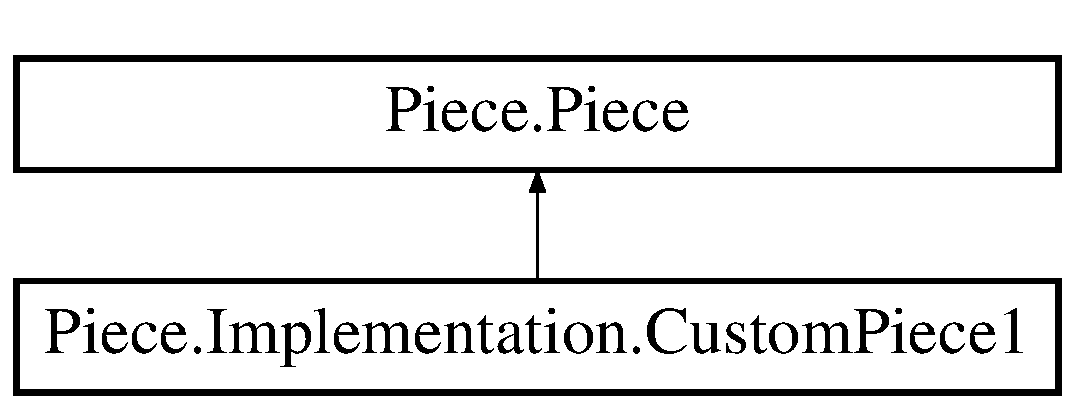
\includegraphics[height=2.000000cm]{classPiece_1_1Implementation_1_1CustomPiece1}
\end{center}
\end{figure}
\subsection*{Public Member Functions}
\begin{DoxyCompactItemize}
\item 
\hyperlink{classPiece_1_1Implementation_1_1CustomPiece1_af3736e05872f710d45a92e303d2efd0f}{Custom\-Piece1} (\hyperlink{classUtil_1_1Position}{Position} start\-Position, int assign\-User\-Id, int assign\-Piece\-Id)  throws Exception
\end{DoxyCompactItemize}
\subsection*{Protected Member Functions}
\begin{DoxyCompactItemize}
\item 
void \hyperlink{classPiece_1_1Implementation_1_1CustomPiece1_aa92e30cda4f19d89b622ec4bf2a6e78e}{init\-Directions} ()  throws Exception 
\end{DoxyCompactItemize}
\subsection*{Additional Inherited Members}


\subsection{Detailed Description}
Class that defines the \hyperlink{classPiece_1_1Implementation_1_1CustomPiece1}{Custom\-Piece1} chess piece. This piece is a mix of knight and bishop pieces \begin{DoxyAuthor}{Author}
Taccio Yamamoto 
\end{DoxyAuthor}


\subsection{Constructor \& Destructor Documentation}
\hypertarget{classPiece_1_1Implementation_1_1CustomPiece1_af3736e05872f710d45a92e303d2efd0f}{\index{Piece\-::\-Implementation\-::\-Custom\-Piece1@{Piece\-::\-Implementation\-::\-Custom\-Piece1}!Custom\-Piece1@{Custom\-Piece1}}
\index{Custom\-Piece1@{Custom\-Piece1}!Piece::Implementation::CustomPiece1@{Piece\-::\-Implementation\-::\-Custom\-Piece1}}
\subsubsection[{Custom\-Piece1}]{\setlength{\rightskip}{0pt plus 5cm}Piece.\-Implementation.\-Custom\-Piece1.\-Custom\-Piece1 (
\begin{DoxyParamCaption}
\item[{{\bf Position}}]{start\-Position, }
\item[{int}]{assign\-User\-Id, }
\item[{int}]{assign\-Piece\-Id}
\end{DoxyParamCaption}
)  throws Exception\hspace{0.3cm}{\ttfamily [inline]}}}\label{classPiece_1_1Implementation_1_1CustomPiece1_af3736e05872f710d45a92e303d2efd0f}
Constructor 
\begin{DoxyParams}{Parameters}
{\em start\-Position} & -\/ start position of the piece \\
\hline
{\em assign\-User\-Id} & -\/ user identification of the owner of the piece \\
\hline
{\em assign\-Piece\-Id} & -\/ unique id assigned to the piece \\
\hline
\end{DoxyParams}

\begin{DoxyExceptions}{Exceptions}
{\em Exception} & throws possible exceptions from the init\-Directions function \\
\hline
\end{DoxyExceptions}


\subsection{Member Function Documentation}
\hypertarget{classPiece_1_1Implementation_1_1CustomPiece1_aa92e30cda4f19d89b622ec4bf2a6e78e}{\index{Piece\-::\-Implementation\-::\-Custom\-Piece1@{Piece\-::\-Implementation\-::\-Custom\-Piece1}!init\-Directions@{init\-Directions}}
\index{init\-Directions@{init\-Directions}!Piece::Implementation::CustomPiece1@{Piece\-::\-Implementation\-::\-Custom\-Piece1}}
\subsubsection[{init\-Directions}]{\setlength{\rightskip}{0pt plus 5cm}void Piece.\-Implementation.\-Custom\-Piece1.\-init\-Directions (
\begin{DoxyParamCaption}
{}
\end{DoxyParamCaption}
)  throws Exception \hspace{0.3cm}{\ttfamily [inline]}, {\ttfamily [protected]}, {\ttfamily [virtual]}}}\label{classPiece_1_1Implementation_1_1CustomPiece1_aa92e30cda4f19d89b622ec4bf2a6e78e}
Initializes the legal directions of the piece 
\begin{DoxyExceptions}{Exceptions}
{\em Exception} & throws exceptions from the Direction constructor \\
\hline
\end{DoxyExceptions}


Implements \hyperlink{classPiece_1_1Piece_af8bf9c4edb5bd73c91f3f8b21793ca5b}{Piece.\-Piece}.



The documentation for this class was generated from the following file\-:\begin{DoxyCompactItemize}
\item 
src/\-Piece/\-Implementation/Custom\-Piece1.\-java\end{DoxyCompactItemize}

\hypertarget{classPiece_1_1Implementation_1_1CustomPiece1Test}{\section{Piece.\-Implementation.\-Custom\-Piece1\-Test Class Reference}
\label{classPiece_1_1Implementation_1_1CustomPiece1Test}\index{Piece.\-Implementation.\-Custom\-Piece1\-Test@{Piece.\-Implementation.\-Custom\-Piece1\-Test}}
}
\subsection*{Public Member Functions}
\begin{DoxyCompactItemize}
\item 
void \hyperlink{classPiece_1_1Implementation_1_1CustomPiece1Test_ae6c652a193ef7c84143df52414c43c74}{set\-Up} ()  throws Exception 
\item 
void \hyperlink{classPiece_1_1Implementation_1_1CustomPiece1Test_a8fe6f1862c04469ec315f147b899b502}{test\-Piece\-Type} ()
\item 
void \hyperlink{classPiece_1_1Implementation_1_1CustomPiece1Test_a746d82cb3a2ab4721ab063d562b29cd5}{test\-Can\-Move} ()  throws Exception
\item 
void \hyperlink{classPiece_1_1Implementation_1_1CustomPiece1Test_a059ef94d70ad425c7dcdf4d26bef54bf}{test\-Move} ()  throws Exception
\item 
void \hyperlink{classPiece_1_1Implementation_1_1CustomPiece1Test_a67af036ffb13cd60098eb39bdcf053a8}{test\-Get\-Functions} ()
\end{DoxyCompactItemize}


\subsection{Detailed Description}
Created by taccio on 2/14/17. 

\subsection{Member Function Documentation}
\hypertarget{classPiece_1_1Implementation_1_1CustomPiece1Test_ae6c652a193ef7c84143df52414c43c74}{\index{Piece\-::\-Implementation\-::\-Custom\-Piece1\-Test@{Piece\-::\-Implementation\-::\-Custom\-Piece1\-Test}!set\-Up@{set\-Up}}
\index{set\-Up@{set\-Up}!Piece::Implementation::CustomPiece1Test@{Piece\-::\-Implementation\-::\-Custom\-Piece1\-Test}}
\subsubsection[{set\-Up}]{\setlength{\rightskip}{0pt plus 5cm}void Piece.\-Implementation.\-Custom\-Piece1\-Test.\-set\-Up (
\begin{DoxyParamCaption}
{}
\end{DoxyParamCaption}
)  throws Exception \hspace{0.3cm}{\ttfamily [inline]}}}\label{classPiece_1_1Implementation_1_1CustomPiece1Test_ae6c652a193ef7c84143df52414c43c74}
Calls setup function before every test function 
\begin{DoxyExceptions}{Exceptions}
{\em Exception} & \\
\hline
\end{DoxyExceptions}
\hypertarget{classPiece_1_1Implementation_1_1CustomPiece1Test_a746d82cb3a2ab4721ab063d562b29cd5}{\index{Piece\-::\-Implementation\-::\-Custom\-Piece1\-Test@{Piece\-::\-Implementation\-::\-Custom\-Piece1\-Test}!test\-Can\-Move@{test\-Can\-Move}}
\index{test\-Can\-Move@{test\-Can\-Move}!Piece::Implementation::CustomPiece1Test@{Piece\-::\-Implementation\-::\-Custom\-Piece1\-Test}}
\subsubsection[{test\-Can\-Move}]{\setlength{\rightskip}{0pt plus 5cm}void Piece.\-Implementation.\-Custom\-Piece1\-Test.\-test\-Can\-Move (
\begin{DoxyParamCaption}
{}
\end{DoxyParamCaption}
)  throws Exception\hspace{0.3cm}{\ttfamily [inline]}}}\label{classPiece_1_1Implementation_1_1CustomPiece1Test_a746d82cb3a2ab4721ab063d562b29cd5}
Tests the can\-Move() function 
\begin{DoxyExceptions}{Exceptions}
{\em Exception} & throws Exception from can\-Move() funciton \\
\hline
\end{DoxyExceptions}
\hypertarget{classPiece_1_1Implementation_1_1CustomPiece1Test_a67af036ffb13cd60098eb39bdcf053a8}{\index{Piece\-::\-Implementation\-::\-Custom\-Piece1\-Test@{Piece\-::\-Implementation\-::\-Custom\-Piece1\-Test}!test\-Get\-Functions@{test\-Get\-Functions}}
\index{test\-Get\-Functions@{test\-Get\-Functions}!Piece::Implementation::CustomPiece1Test@{Piece\-::\-Implementation\-::\-Custom\-Piece1\-Test}}
\subsubsection[{test\-Get\-Functions}]{\setlength{\rightskip}{0pt plus 5cm}void Piece.\-Implementation.\-Custom\-Piece1\-Test.\-test\-Get\-Functions (
\begin{DoxyParamCaption}
{}
\end{DoxyParamCaption}
)\hspace{0.3cm}{\ttfamily [inline]}}}\label{classPiece_1_1Implementation_1_1CustomPiece1Test_a67af036ffb13cd60098eb39bdcf053a8}
Tests different Get funcitons \hypertarget{classPiece_1_1Implementation_1_1CustomPiece1Test_a059ef94d70ad425c7dcdf4d26bef54bf}{\index{Piece\-::\-Implementation\-::\-Custom\-Piece1\-Test@{Piece\-::\-Implementation\-::\-Custom\-Piece1\-Test}!test\-Move@{test\-Move}}
\index{test\-Move@{test\-Move}!Piece::Implementation::CustomPiece1Test@{Piece\-::\-Implementation\-::\-Custom\-Piece1\-Test}}
\subsubsection[{test\-Move}]{\setlength{\rightskip}{0pt plus 5cm}void Piece.\-Implementation.\-Custom\-Piece1\-Test.\-test\-Move (
\begin{DoxyParamCaption}
{}
\end{DoxyParamCaption}
)  throws Exception\hspace{0.3cm}{\ttfamily [inline]}}}\label{classPiece_1_1Implementation_1_1CustomPiece1Test_a059ef94d70ad425c7dcdf4d26bef54bf}
Tests the move() function 
\begin{DoxyExceptions}{Exceptions}
{\em Exception} & throws Exception from move() funciton \\
\hline
\end{DoxyExceptions}
\hypertarget{classPiece_1_1Implementation_1_1CustomPiece1Test_a8fe6f1862c04469ec315f147b899b502}{\index{Piece\-::\-Implementation\-::\-Custom\-Piece1\-Test@{Piece\-::\-Implementation\-::\-Custom\-Piece1\-Test}!test\-Piece\-Type@{test\-Piece\-Type}}
\index{test\-Piece\-Type@{test\-Piece\-Type}!Piece::Implementation::CustomPiece1Test@{Piece\-::\-Implementation\-::\-Custom\-Piece1\-Test}}
\subsubsection[{test\-Piece\-Type}]{\setlength{\rightskip}{0pt plus 5cm}void Piece.\-Implementation.\-Custom\-Piece1\-Test.\-test\-Piece\-Type (
\begin{DoxyParamCaption}
{}
\end{DoxyParamCaption}
)\hspace{0.3cm}{\ttfamily [inline]}}}\label{classPiece_1_1Implementation_1_1CustomPiece1Test_a8fe6f1862c04469ec315f147b899b502}
Checks the piece has correct \hyperlink{enumPiece_1_1PieceType}{Piece\-Type} 

The documentation for this class was generated from the following file\-:\begin{DoxyCompactItemize}
\item 
test/\-Piece/\-Implementation/Custom\-Piece1\-Test.\-java\end{DoxyCompactItemize}

\hypertarget{classPiece_1_1Implementation_1_1CustomPiece2}{\section{Piece.\-Implementation.\-Custom\-Piece2 Class Reference}
\label{classPiece_1_1Implementation_1_1CustomPiece2}\index{Piece.\-Implementation.\-Custom\-Piece2@{Piece.\-Implementation.\-Custom\-Piece2}}
}
Inheritance diagram for Piece.\-Implementation.\-Custom\-Piece2\-:\begin{figure}[H]
\begin{center}
\leavevmode
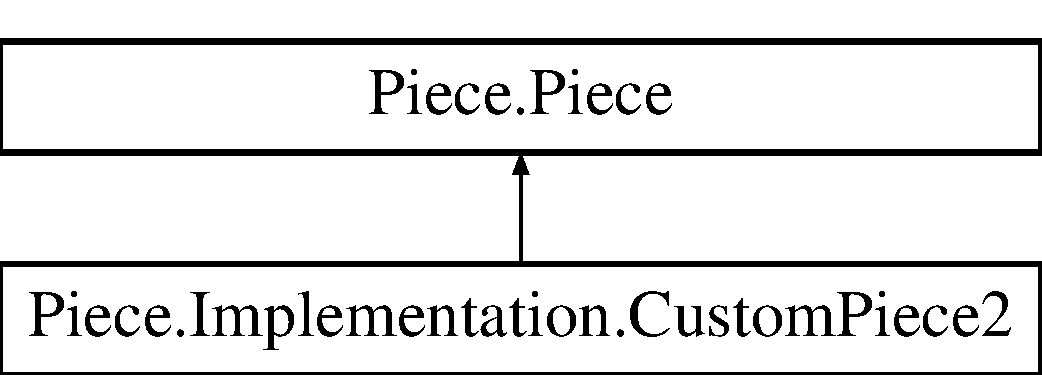
\includegraphics[height=2.000000cm]{classPiece_1_1Implementation_1_1CustomPiece2}
\end{center}
\end{figure}
\subsection*{Public Member Functions}
\begin{DoxyCompactItemize}
\item 
\hyperlink{classPiece_1_1Implementation_1_1CustomPiece2_a749428618cabbb98dbe08d465abf25d5}{Custom\-Piece2} (\hyperlink{classUtil_1_1Position}{Position} start\-Position, int assign\-User\-Id, int assign\-Piece\-Id)  throws Exception
\end{DoxyCompactItemize}
\subsection*{Protected Member Functions}
\begin{DoxyCompactItemize}
\item 
void \hyperlink{classPiece_1_1Implementation_1_1CustomPiece2_a33801c7e929e4ab100dd23c053c98dba}{init\-Directions} ()  throws Exception 
\end{DoxyCompactItemize}
\subsection*{Additional Inherited Members}


\subsection{Detailed Description}
Class that defines the \hyperlink{classPiece_1_1Implementation_1_1CustomPiece2}{Custom\-Piece2} chess piece. This piece can move up to 2 squares in any direction \begin{DoxyAuthor}{Author}
Taccio Yamamoto 
\end{DoxyAuthor}


\subsection{Constructor \& Destructor Documentation}
\hypertarget{classPiece_1_1Implementation_1_1CustomPiece2_a749428618cabbb98dbe08d465abf25d5}{\index{Piece\-::\-Implementation\-::\-Custom\-Piece2@{Piece\-::\-Implementation\-::\-Custom\-Piece2}!Custom\-Piece2@{Custom\-Piece2}}
\index{Custom\-Piece2@{Custom\-Piece2}!Piece::Implementation::CustomPiece2@{Piece\-::\-Implementation\-::\-Custom\-Piece2}}
\subsubsection[{Custom\-Piece2}]{\setlength{\rightskip}{0pt plus 5cm}Piece.\-Implementation.\-Custom\-Piece2.\-Custom\-Piece2 (
\begin{DoxyParamCaption}
\item[{{\bf Position}}]{start\-Position, }
\item[{int}]{assign\-User\-Id, }
\item[{int}]{assign\-Piece\-Id}
\end{DoxyParamCaption}
)  throws Exception\hspace{0.3cm}{\ttfamily [inline]}}}\label{classPiece_1_1Implementation_1_1CustomPiece2_a749428618cabbb98dbe08d465abf25d5}
Constructor 
\begin{DoxyParams}{Parameters}
{\em start\-Position} & -\/ start position of the piece \\
\hline
{\em assign\-User\-Id} & -\/ user identification of the owner of the piece \\
\hline
{\em assign\-Piece\-Id} & -\/ unique id assigned to the piece \\
\hline
\end{DoxyParams}

\begin{DoxyExceptions}{Exceptions}
{\em Exception} & throws possible exceptions from the init\-Directions function \\
\hline
\end{DoxyExceptions}


\subsection{Member Function Documentation}
\hypertarget{classPiece_1_1Implementation_1_1CustomPiece2_a33801c7e929e4ab100dd23c053c98dba}{\index{Piece\-::\-Implementation\-::\-Custom\-Piece2@{Piece\-::\-Implementation\-::\-Custom\-Piece2}!init\-Directions@{init\-Directions}}
\index{init\-Directions@{init\-Directions}!Piece::Implementation::CustomPiece2@{Piece\-::\-Implementation\-::\-Custom\-Piece2}}
\subsubsection[{init\-Directions}]{\setlength{\rightskip}{0pt plus 5cm}void Piece.\-Implementation.\-Custom\-Piece2.\-init\-Directions (
\begin{DoxyParamCaption}
{}
\end{DoxyParamCaption}
)  throws Exception \hspace{0.3cm}{\ttfamily [inline]}, {\ttfamily [protected]}, {\ttfamily [virtual]}}}\label{classPiece_1_1Implementation_1_1CustomPiece2_a33801c7e929e4ab100dd23c053c98dba}
Initializes the legal directions of the piece 
\begin{DoxyExceptions}{Exceptions}
{\em Exception} & throws exceptions from the Direction constructor \\
\hline
\end{DoxyExceptions}


Implements \hyperlink{classPiece_1_1Piece_af8bf9c4edb5bd73c91f3f8b21793ca5b}{Piece.\-Piece}.



The documentation for this class was generated from the following file\-:\begin{DoxyCompactItemize}
\item 
src/\-Piece/\-Implementation/Custom\-Piece2.\-java\end{DoxyCompactItemize}

\hypertarget{classPiece_1_1Implementation_1_1CustomPiece2Test}{\section{Piece.\-Implementation.\-Custom\-Piece2\-Test Class Reference}
\label{classPiece_1_1Implementation_1_1CustomPiece2Test}\index{Piece.\-Implementation.\-Custom\-Piece2\-Test@{Piece.\-Implementation.\-Custom\-Piece2\-Test}}
}
\subsection*{Public Member Functions}
\begin{DoxyCompactItemize}
\item 
void \hyperlink{classPiece_1_1Implementation_1_1CustomPiece2Test_a4ebb52055472a7626562c9706eeca579}{set\-Up} ()  throws Exception 
\item 
void \hyperlink{classPiece_1_1Implementation_1_1CustomPiece2Test_a0388f0ad766b662b9bc875166c85df8c}{test\-Piece\-Type} ()
\item 
void \hyperlink{classPiece_1_1Implementation_1_1CustomPiece2Test_ab3c717c9cd78e9a8fe91e95d63bfcf1e}{test\-Can\-Move} ()  throws Exception
\item 
void \hyperlink{classPiece_1_1Implementation_1_1CustomPiece2Test_a5f6e2e14e6a8f1c631d30b5f1a68707a}{test\-Move} ()  throws Exception
\item 
void \hyperlink{classPiece_1_1Implementation_1_1CustomPiece2Test_afdaa72c5ea2ec0d4ec336ca9e37307ee}{test\-Get\-Functions} ()
\end{DoxyCompactItemize}


\subsection{Detailed Description}
Created by taccio on 2/14/17. 

\subsection{Member Function Documentation}
\hypertarget{classPiece_1_1Implementation_1_1CustomPiece2Test_a4ebb52055472a7626562c9706eeca579}{\index{Piece\-::\-Implementation\-::\-Custom\-Piece2\-Test@{Piece\-::\-Implementation\-::\-Custom\-Piece2\-Test}!set\-Up@{set\-Up}}
\index{set\-Up@{set\-Up}!Piece::Implementation::CustomPiece2Test@{Piece\-::\-Implementation\-::\-Custom\-Piece2\-Test}}
\subsubsection[{set\-Up}]{\setlength{\rightskip}{0pt plus 5cm}void Piece.\-Implementation.\-Custom\-Piece2\-Test.\-set\-Up (
\begin{DoxyParamCaption}
{}
\end{DoxyParamCaption}
)  throws Exception \hspace{0.3cm}{\ttfamily [inline]}}}\label{classPiece_1_1Implementation_1_1CustomPiece2Test_a4ebb52055472a7626562c9706eeca579}
Calls setup function before every test function 
\begin{DoxyExceptions}{Exceptions}
{\em Exception} & \\
\hline
\end{DoxyExceptions}
\hypertarget{classPiece_1_1Implementation_1_1CustomPiece2Test_ab3c717c9cd78e9a8fe91e95d63bfcf1e}{\index{Piece\-::\-Implementation\-::\-Custom\-Piece2\-Test@{Piece\-::\-Implementation\-::\-Custom\-Piece2\-Test}!test\-Can\-Move@{test\-Can\-Move}}
\index{test\-Can\-Move@{test\-Can\-Move}!Piece::Implementation::CustomPiece2Test@{Piece\-::\-Implementation\-::\-Custom\-Piece2\-Test}}
\subsubsection[{test\-Can\-Move}]{\setlength{\rightskip}{0pt plus 5cm}void Piece.\-Implementation.\-Custom\-Piece2\-Test.\-test\-Can\-Move (
\begin{DoxyParamCaption}
{}
\end{DoxyParamCaption}
)  throws Exception\hspace{0.3cm}{\ttfamily [inline]}}}\label{classPiece_1_1Implementation_1_1CustomPiece2Test_ab3c717c9cd78e9a8fe91e95d63bfcf1e}
Tests the can\-Move() function 
\begin{DoxyExceptions}{Exceptions}
{\em Exception} & throws Exception from can\-Move() funciton \\
\hline
\end{DoxyExceptions}
\hypertarget{classPiece_1_1Implementation_1_1CustomPiece2Test_afdaa72c5ea2ec0d4ec336ca9e37307ee}{\index{Piece\-::\-Implementation\-::\-Custom\-Piece2\-Test@{Piece\-::\-Implementation\-::\-Custom\-Piece2\-Test}!test\-Get\-Functions@{test\-Get\-Functions}}
\index{test\-Get\-Functions@{test\-Get\-Functions}!Piece::Implementation::CustomPiece2Test@{Piece\-::\-Implementation\-::\-Custom\-Piece2\-Test}}
\subsubsection[{test\-Get\-Functions}]{\setlength{\rightskip}{0pt plus 5cm}void Piece.\-Implementation.\-Custom\-Piece2\-Test.\-test\-Get\-Functions (
\begin{DoxyParamCaption}
{}
\end{DoxyParamCaption}
)\hspace{0.3cm}{\ttfamily [inline]}}}\label{classPiece_1_1Implementation_1_1CustomPiece2Test_afdaa72c5ea2ec0d4ec336ca9e37307ee}
Tests different Get funcitons \hypertarget{classPiece_1_1Implementation_1_1CustomPiece2Test_a5f6e2e14e6a8f1c631d30b5f1a68707a}{\index{Piece\-::\-Implementation\-::\-Custom\-Piece2\-Test@{Piece\-::\-Implementation\-::\-Custom\-Piece2\-Test}!test\-Move@{test\-Move}}
\index{test\-Move@{test\-Move}!Piece::Implementation::CustomPiece2Test@{Piece\-::\-Implementation\-::\-Custom\-Piece2\-Test}}
\subsubsection[{test\-Move}]{\setlength{\rightskip}{0pt plus 5cm}void Piece.\-Implementation.\-Custom\-Piece2\-Test.\-test\-Move (
\begin{DoxyParamCaption}
{}
\end{DoxyParamCaption}
)  throws Exception\hspace{0.3cm}{\ttfamily [inline]}}}\label{classPiece_1_1Implementation_1_1CustomPiece2Test_a5f6e2e14e6a8f1c631d30b5f1a68707a}
Tests the move() function 
\begin{DoxyExceptions}{Exceptions}
{\em Exception} & throws Exception from move() funciton \\
\hline
\end{DoxyExceptions}
\hypertarget{classPiece_1_1Implementation_1_1CustomPiece2Test_a0388f0ad766b662b9bc875166c85df8c}{\index{Piece\-::\-Implementation\-::\-Custom\-Piece2\-Test@{Piece\-::\-Implementation\-::\-Custom\-Piece2\-Test}!test\-Piece\-Type@{test\-Piece\-Type}}
\index{test\-Piece\-Type@{test\-Piece\-Type}!Piece::Implementation::CustomPiece2Test@{Piece\-::\-Implementation\-::\-Custom\-Piece2\-Test}}
\subsubsection[{test\-Piece\-Type}]{\setlength{\rightskip}{0pt plus 5cm}void Piece.\-Implementation.\-Custom\-Piece2\-Test.\-test\-Piece\-Type (
\begin{DoxyParamCaption}
{}
\end{DoxyParamCaption}
)\hspace{0.3cm}{\ttfamily [inline]}}}\label{classPiece_1_1Implementation_1_1CustomPiece2Test_a0388f0ad766b662b9bc875166c85df8c}
Checks the piece has correct \hyperlink{enumPiece_1_1PieceType}{Piece\-Type} 

The documentation for this class was generated from the following file\-:\begin{DoxyCompactItemize}
\item 
test/\-Piece/\-Implementation/Custom\-Piece2\-Test.\-java\end{DoxyCompactItemize}

\hypertarget{classUtil_1_1Direction}{\section{Util.\-Direction Class Reference}
\label{classUtil_1_1Direction}\index{Util.\-Direction@{Util.\-Direction}}
}
\subsection*{Public Member Functions}
\begin{DoxyCompactItemize}
\item 
\hyperlink{classUtil_1_1Direction_a4d016d4fe73c7c69bc0474ca3544e229}{Direction} (int dx, int dy, int distance)  throws Exception 
\item 
\hyperlink{classUtil_1_1Direction_aca0d10a0f6f1cab6b6453442db88ac41}{Direction} (int\mbox{[}$\,$\mbox{]} dir\-Vector, int distance)  throws Exception
\item 
\hyperlink{classUtil_1_1Direction_a96dc3c7b359455ce714e2a4fb3aa9f93}{Direction} (\hyperlink{classUtil_1_1Direction}{Direction} copy\-Dir)  throws Exception
\item 
\hyperlink{classUtil_1_1Direction_ab6cd1dac79dbe582e8d671c86be71244}{Direction} (\hyperlink{classUtil_1_1Position}{Position} initial, \hyperlink{classUtil_1_1Position}{Position} end, int distance)  throws Exception
\item 
int\mbox{[}$\,$\mbox{]} \hyperlink{classUtil_1_1Direction_aec2a7a04741e2ef55d74f4635348cad3}{get\-Direction} ()
\item 
void \hyperlink{classUtil_1_1Direction_a0938e111d70b74e80faceba0f5146e17}{set\-Direction} (\hyperlink{classUtil_1_1Direction}{Direction} new\-Direction)
\item 
boolean \hyperlink{classUtil_1_1Direction_a8a6d78e18b047715a38078781b1fb813}{can\-Move\-In\-Direction} (\hyperlink{classUtil_1_1Position}{Position} current\-Position, \hyperlink{classUtil_1_1Position}{Position} target\-Position, \hyperlink{classBoard_1_1Board}{Board} board)  throws Exception
\item 
int \hyperlink{classUtil_1_1Direction_a5f52ca9bceaa59fc2afad1f87c5500ee}{get\-Distance} ()
\item 
void \hyperlink{classUtil_1_1Direction_aa5997dad71c8217853d08bd5987bfc61}{set\-Distance} (int distance)  throws Exception
\item 
void \hyperlink{classUtil_1_1Direction_aca852c23943cb0e955a5fe4aff888935}{set\-Direction} (int dx, int dy)
\item 
void \hyperlink{classUtil_1_1Direction_a0f498a800bfb0416047d0aafe12b5692}{set\-Direction} (int\mbox{[}$\,$\mbox{]} direction\-Arr)
\item 
void \hyperlink{classUtil_1_1Direction_af1244167566f6eb257798fd2d45012b5}{set\-Direction} (\hyperlink{classUtil_1_1Position}{Position} initial, \hyperlink{classUtil_1_1Position}{Position} end)  throws Exception 
\item 
boolean \hyperlink{classUtil_1_1Direction_aca147d8964ccb5618198c359998a6635}{equals} (\hyperlink{classUtil_1_1Direction}{Direction} other\-Direction)
\end{DoxyCompactItemize}


\subsection{Detailed Description}
Class to handle directions of each piece \begin{DoxyAuthor}{Author}
Taccio Yamamoto 
\end{DoxyAuthor}


\subsection{Constructor \& Destructor Documentation}
\hypertarget{classUtil_1_1Direction_a4d016d4fe73c7c69bc0474ca3544e229}{\index{Util\-::\-Direction@{Util\-::\-Direction}!Direction@{Direction}}
\index{Direction@{Direction}!Util::Direction@{Util\-::\-Direction}}
\subsubsection[{Direction}]{\setlength{\rightskip}{0pt plus 5cm}Util.\-Direction.\-Direction (
\begin{DoxyParamCaption}
\item[{int}]{dx, }
\item[{int}]{dy, }
\item[{int}]{distance}
\end{DoxyParamCaption}
)  throws Exception \hspace{0.3cm}{\ttfamily [inline]}}}\label{classUtil_1_1Direction_a4d016d4fe73c7c69bc0474ca3544e229}
Constructor to create direction objects 
\begin{DoxyParams}{Parameters}
{\em dx} & -\/ row vector \\
\hline
{\em dy} & -\/ column vector \\
\hline
{\em distance} & -\/ distance piece can move, -\/1 if piece can move infinitely long until it reaches another piece \\
\hline
\end{DoxyParams}
\hypertarget{classUtil_1_1Direction_aca0d10a0f6f1cab6b6453442db88ac41}{\index{Util\-::\-Direction@{Util\-::\-Direction}!Direction@{Direction}}
\index{Direction@{Direction}!Util::Direction@{Util\-::\-Direction}}
\subsubsection[{Direction}]{\setlength{\rightskip}{0pt plus 5cm}Util.\-Direction.\-Direction (
\begin{DoxyParamCaption}
\item[{int\mbox{[}$\,$\mbox{]}}]{dir\-Vector, }
\item[{int}]{distance}
\end{DoxyParamCaption}
)  throws Exception\hspace{0.3cm}{\ttfamily [inline]}}}\label{classUtil_1_1Direction_aca0d10a0f6f1cab6b6453442db88ac41}
Constructor to create direction objects 
\begin{DoxyParams}{Parameters}
{\em dir\-Vector} & -\/ direction vector to assign to dir\-Vector \\
\hline
{\em distance} & -\/ distance piece can move, -\/1 if piece can move infinitely long until it reaches another piece \\
\hline
\end{DoxyParams}
\hypertarget{classUtil_1_1Direction_a96dc3c7b359455ce714e2a4fb3aa9f93}{\index{Util\-::\-Direction@{Util\-::\-Direction}!Direction@{Direction}}
\index{Direction@{Direction}!Util::Direction@{Util\-::\-Direction}}
\subsubsection[{Direction}]{\setlength{\rightskip}{0pt plus 5cm}Util.\-Direction.\-Direction (
\begin{DoxyParamCaption}
\item[{{\bf Direction}}]{copy\-Dir}
\end{DoxyParamCaption}
)  throws Exception\hspace{0.3cm}{\ttfamily [inline]}}}\label{classUtil_1_1Direction_a96dc3c7b359455ce714e2a4fb3aa9f93}
Constructor to create direction objects 
\begin{DoxyParams}{Parameters}
{\em copy\-Dir} & -\/ \hyperlink{classUtil_1_1Direction}{Direction} to copy from \\
\hline
\end{DoxyParams}
\hypertarget{classUtil_1_1Direction_ab6cd1dac79dbe582e8d671c86be71244}{\index{Util\-::\-Direction@{Util\-::\-Direction}!Direction@{Direction}}
\index{Direction@{Direction}!Util::Direction@{Util\-::\-Direction}}
\subsubsection[{Direction}]{\setlength{\rightskip}{0pt plus 5cm}Util.\-Direction.\-Direction (
\begin{DoxyParamCaption}
\item[{{\bf Position}}]{initial, }
\item[{{\bf Position}}]{end, }
\item[{int}]{distance}
\end{DoxyParamCaption}
)  throws Exception\hspace{0.3cm}{\ttfamily [inline]}}}\label{classUtil_1_1Direction_ab6cd1dac79dbe582e8d671c86be71244}
Constructor to create direction objects from position objects 
\begin{DoxyParams}{Parameters}
{\em initial} & -\/ initial position \\
\hline
{\em end} & -\/ end position \\
\hline
{\em distance} & -\/ distance piece can move, -\/1 if piece can move infinitely long until it reaches another piece \\
\hline
\end{DoxyParams}


\subsection{Member Function Documentation}
\hypertarget{classUtil_1_1Direction_a8a6d78e18b047715a38078781b1fb813}{\index{Util\-::\-Direction@{Util\-::\-Direction}!can\-Move\-In\-Direction@{can\-Move\-In\-Direction}}
\index{can\-Move\-In\-Direction@{can\-Move\-In\-Direction}!Util::Direction@{Util\-::\-Direction}}
\subsubsection[{can\-Move\-In\-Direction}]{\setlength{\rightskip}{0pt plus 5cm}boolean Util.\-Direction.\-can\-Move\-In\-Direction (
\begin{DoxyParamCaption}
\item[{{\bf Position}}]{current\-Position, }
\item[{{\bf Position}}]{target\-Position, }
\item[{{\bf Board}}]{board}
\end{DoxyParamCaption}
)  throws Exception\hspace{0.3cm}{\ttfamily [inline]}}}\label{classUtil_1_1Direction_a8a6d78e18b047715a38078781b1fb813}
Checks if the Direcion object allows to move from current\-Position to target\-Position. 
\begin{DoxyParams}{Parameters}
{\em current\-Position} & -\/ current position \\
\hline
{\em target\-Position} & -\/ target position \\
\hline
{\em board} & -\/ board object that keeps track of all the pieces \\
\hline
\end{DoxyParams}
\begin{DoxyReturn}{Returns}
true if the \hyperlink{classUtil_1_1Direction}{Direction} object can move from the current\-Position to the target\-Position 
\end{DoxyReturn}
\hypertarget{classUtil_1_1Direction_aca147d8964ccb5618198c359998a6635}{\index{Util\-::\-Direction@{Util\-::\-Direction}!equals@{equals}}
\index{equals@{equals}!Util::Direction@{Util\-::\-Direction}}
\subsubsection[{equals}]{\setlength{\rightskip}{0pt plus 5cm}boolean Util.\-Direction.\-equals (
\begin{DoxyParamCaption}
\item[{{\bf Direction}}]{other\-Direction}
\end{DoxyParamCaption}
)\hspace{0.3cm}{\ttfamily [inline]}}}\label{classUtil_1_1Direction_aca147d8964ccb5618198c359998a6635}
Checks if the two \hyperlink{classUtil_1_1Direction}{Direction} objects have the same direction vector 
\begin{DoxyParams}{Parameters}
{\em other\-Direction} & \hyperlink{classUtil_1_1Direction}{Direction} object to compare to \\
\hline
\end{DoxyParams}
\begin{DoxyReturn}{Returns}
boolean ths is true if both \hyperlink{classUtil_1_1Direction}{Direction} objects has the same direction 
\end{DoxyReturn}
\hypertarget{classUtil_1_1Direction_aec2a7a04741e2ef55d74f4635348cad3}{\index{Util\-::\-Direction@{Util\-::\-Direction}!get\-Direction@{get\-Direction}}
\index{get\-Direction@{get\-Direction}!Util::Direction@{Util\-::\-Direction}}
\subsubsection[{get\-Direction}]{\setlength{\rightskip}{0pt plus 5cm}int \mbox{[}$\,$\mbox{]} Util.\-Direction.\-get\-Direction (
\begin{DoxyParamCaption}
{}
\end{DoxyParamCaption}
)\hspace{0.3cm}{\ttfamily [inline]}}}\label{classUtil_1_1Direction_aec2a7a04741e2ef55d74f4635348cad3}
Returns direction vector \begin{DoxyReturn}{Returns}
int\mbox{[}\mbox{]} array of the direction vector 
\end{DoxyReturn}
\hypertarget{classUtil_1_1Direction_a5f52ca9bceaa59fc2afad1f87c5500ee}{\index{Util\-::\-Direction@{Util\-::\-Direction}!get\-Distance@{get\-Distance}}
\index{get\-Distance@{get\-Distance}!Util::Direction@{Util\-::\-Direction}}
\subsubsection[{get\-Distance}]{\setlength{\rightskip}{0pt plus 5cm}int Util.\-Direction.\-get\-Distance (
\begin{DoxyParamCaption}
{}
\end{DoxyParamCaption}
)\hspace{0.3cm}{\ttfamily [inline]}}}\label{classUtil_1_1Direction_a5f52ca9bceaa59fc2afad1f87c5500ee}
Get distance function \begin{DoxyReturn}{Returns}
distance piece can move, -\/1 if piece can move infinitely long until it reaches another piece 
\end{DoxyReturn}
\hypertarget{classUtil_1_1Direction_a0938e111d70b74e80faceba0f5146e17}{\index{Util\-::\-Direction@{Util\-::\-Direction}!set\-Direction@{set\-Direction}}
\index{set\-Direction@{set\-Direction}!Util::Direction@{Util\-::\-Direction}}
\subsubsection[{set\-Direction}]{\setlength{\rightskip}{0pt plus 5cm}void Util.\-Direction.\-set\-Direction (
\begin{DoxyParamCaption}
\item[{{\bf Direction}}]{new\-Direction}
\end{DoxyParamCaption}
)\hspace{0.3cm}{\ttfamily [inline]}}}\label{classUtil_1_1Direction_a0938e111d70b74e80faceba0f5146e17}
Sets the direction vector 
\begin{DoxyParams}{Parameters}
{\em new\-Direction} & -\/ \hyperlink{classUtil_1_1Direction}{Direction} object to copy from \\
\hline
\end{DoxyParams}
\hypertarget{classUtil_1_1Direction_aca852c23943cb0e955a5fe4aff888935}{\index{Util\-::\-Direction@{Util\-::\-Direction}!set\-Direction@{set\-Direction}}
\index{set\-Direction@{set\-Direction}!Util::Direction@{Util\-::\-Direction}}
\subsubsection[{set\-Direction}]{\setlength{\rightskip}{0pt plus 5cm}void Util.\-Direction.\-set\-Direction (
\begin{DoxyParamCaption}
\item[{int}]{dx, }
\item[{int}]{dy}
\end{DoxyParamCaption}
)\hspace{0.3cm}{\ttfamily [inline]}}}\label{classUtil_1_1Direction_aca852c23943cb0e955a5fe4aff888935}
Sets the direction vector 
\begin{DoxyParams}{Parameters}
{\em dx} & -\/ row vector \\
\hline
{\em dy} & -\/ column vector \\
\hline
\end{DoxyParams}
\hypertarget{classUtil_1_1Direction_a0f498a800bfb0416047d0aafe12b5692}{\index{Util\-::\-Direction@{Util\-::\-Direction}!set\-Direction@{set\-Direction}}
\index{set\-Direction@{set\-Direction}!Util::Direction@{Util\-::\-Direction}}
\subsubsection[{set\-Direction}]{\setlength{\rightskip}{0pt plus 5cm}void Util.\-Direction.\-set\-Direction (
\begin{DoxyParamCaption}
\item[{int\mbox{[}$\,$\mbox{]}}]{direction\-Arr}
\end{DoxyParamCaption}
)\hspace{0.3cm}{\ttfamily [inline]}}}\label{classUtil_1_1Direction_a0f498a800bfb0416047d0aafe12b5692}
Sets the direction vector 
\begin{DoxyParams}{Parameters}
{\em direction\-Arr} & -\/ direction vector to set \\
\hline
\end{DoxyParams}
\hypertarget{classUtil_1_1Direction_af1244167566f6eb257798fd2d45012b5}{\index{Util\-::\-Direction@{Util\-::\-Direction}!set\-Direction@{set\-Direction}}
\index{set\-Direction@{set\-Direction}!Util::Direction@{Util\-::\-Direction}}
\subsubsection[{set\-Direction}]{\setlength{\rightskip}{0pt plus 5cm}void Util.\-Direction.\-set\-Direction (
\begin{DoxyParamCaption}
\item[{{\bf Position}}]{initial, }
\item[{{\bf Position}}]{end}
\end{DoxyParamCaption}
)  throws Exception \hspace{0.3cm}{\ttfamily [inline]}}}\label{classUtil_1_1Direction_af1244167566f6eb257798fd2d45012b5}
Sets the direction vector 
\begin{DoxyParams}{Parameters}
{\em initial} & -\/ initial \hyperlink{classUtil_1_1Position}{Position} object \\
\hline
{\em end} & -\/ final \hyperlink{classUtil_1_1Position}{Position} object \\
\hline
\end{DoxyParams}

\begin{DoxyExceptions}{Exceptions}
{\em Exception} & -\/ throws exception if the positions have different array lengths \\
\hline
\end{DoxyExceptions}
\hypertarget{classUtil_1_1Direction_aa5997dad71c8217853d08bd5987bfc61}{\index{Util\-::\-Direction@{Util\-::\-Direction}!set\-Distance@{set\-Distance}}
\index{set\-Distance@{set\-Distance}!Util::Direction@{Util\-::\-Direction}}
\subsubsection[{set\-Distance}]{\setlength{\rightskip}{0pt plus 5cm}void Util.\-Direction.\-set\-Distance (
\begin{DoxyParamCaption}
\item[{int}]{distance}
\end{DoxyParamCaption}
)  throws Exception\hspace{0.3cm}{\ttfamily [inline]}}}\label{classUtil_1_1Direction_aa5997dad71c8217853d08bd5987bfc61}
Sets the distance function 
\begin{DoxyParams}{Parameters}
{\em distance} & -\/ new distance, -\/1 if piece can move infinitely long until it reaches another piece \\
\hline
\end{DoxyParams}


The documentation for this class was generated from the following file\-:\begin{DoxyCompactItemize}
\item 
src/\-Util/Direction.\-java\end{DoxyCompactItemize}

\hypertarget{classUtil_1_1DirectionTest}{\section{Util.\-Direction\-Test Class Reference}
\label{classUtil_1_1DirectionTest}\index{Util.\-Direction\-Test@{Util.\-Direction\-Test}}
}
\subsection*{Public Member Functions}
\begin{DoxyCompactItemize}
\item 
void \hyperlink{classUtil_1_1DirectionTest_a900dfa1061295fe5c0cf7ec46b5f977c}{test\-Constructors} ()  throws Exception 
\item 
void \hyperlink{classUtil_1_1DirectionTest_acd30575c3cbfe9061181062287ecde95}{get\-Direction} ()  throws Exception 
\item 
void \hyperlink{classUtil_1_1DirectionTest_a3022a5ee6ca90a97ac9264e9e77c1ef9}{set\-Direction} ()  throws Exception 
\item 
void \hyperlink{classUtil_1_1DirectionTest_ac54b71f3e0e11db7cd13513b4def3133}{equals} ()  throws Exception 
\item 
\hypertarget{classUtil_1_1DirectionTest_a87869fbff63da2f1af7911c6b0eafa77}{void {\bfseries move\-By\-Direction} ()  throws Exception }\label{classUtil_1_1DirectionTest_a87869fbff63da2f1af7911c6b0eafa77}

\item 
void \hyperlink{classUtil_1_1DirectionTest_a5430dba55b03913a6c1b567fa3700b9a}{can\-Move} ()  throws Exception
\end{DoxyCompactItemize}


\subsection{Detailed Description}
Created by taccio on 2/12/17. 

\subsection{Member Function Documentation}
\hypertarget{classUtil_1_1DirectionTest_a5430dba55b03913a6c1b567fa3700b9a}{\index{Util\-::\-Direction\-Test@{Util\-::\-Direction\-Test}!can\-Move@{can\-Move}}
\index{can\-Move@{can\-Move}!Util::DirectionTest@{Util\-::\-Direction\-Test}}
\subsubsection[{can\-Move}]{\setlength{\rightskip}{0pt plus 5cm}void Util.\-Direction\-Test.\-can\-Move (
\begin{DoxyParamCaption}
{}
\end{DoxyParamCaption}
)  throws Exception\hspace{0.3cm}{\ttfamily [inline]}}}\label{classUtil_1_1DirectionTest_a5430dba55b03913a6c1b567fa3700b9a}

\begin{DoxyExceptions}{Exceptions}
{\em Exception} & \\
\hline
\end{DoxyExceptions}
\hypertarget{classUtil_1_1DirectionTest_ac54b71f3e0e11db7cd13513b4def3133}{\index{Util\-::\-Direction\-Test@{Util\-::\-Direction\-Test}!equals@{equals}}
\index{equals@{equals}!Util::DirectionTest@{Util\-::\-Direction\-Test}}
\subsubsection[{equals}]{\setlength{\rightskip}{0pt plus 5cm}void Util.\-Direction\-Test.\-equals (
\begin{DoxyParamCaption}
{}
\end{DoxyParamCaption}
)  throws Exception \hspace{0.3cm}{\ttfamily [inline]}}}\label{classUtil_1_1DirectionTest_ac54b71f3e0e11db7cd13513b4def3133}
Tests \hyperlink{classUtil_1_1DirectionTest_ac54b71f3e0e11db7cd13513b4def3133}{equals()} function 
\begin{DoxyExceptions}{Exceptions}
{\em Exception} & \\
\hline
\end{DoxyExceptions}
\hypertarget{classUtil_1_1DirectionTest_acd30575c3cbfe9061181062287ecde95}{\index{Util\-::\-Direction\-Test@{Util\-::\-Direction\-Test}!get\-Direction@{get\-Direction}}
\index{get\-Direction@{get\-Direction}!Util::DirectionTest@{Util\-::\-Direction\-Test}}
\subsubsection[{get\-Direction}]{\setlength{\rightskip}{0pt plus 5cm}void Util.\-Direction\-Test.\-get\-Direction (
\begin{DoxyParamCaption}
{}
\end{DoxyParamCaption}
)  throws Exception \hspace{0.3cm}{\ttfamily [inline]}}}\label{classUtil_1_1DirectionTest_acd30575c3cbfe9061181062287ecde95}
Tests the get\-Direction method 
\begin{DoxyExceptions}{Exceptions}
{\em Exception} & \\
\hline
\end{DoxyExceptions}
\hypertarget{classUtil_1_1DirectionTest_a3022a5ee6ca90a97ac9264e9e77c1ef9}{\index{Util\-::\-Direction\-Test@{Util\-::\-Direction\-Test}!set\-Direction@{set\-Direction}}
\index{set\-Direction@{set\-Direction}!Util::DirectionTest@{Util\-::\-Direction\-Test}}
\subsubsection[{set\-Direction}]{\setlength{\rightskip}{0pt plus 5cm}void Util.\-Direction\-Test.\-set\-Direction (
\begin{DoxyParamCaption}
{}
\end{DoxyParamCaption}
)  throws Exception \hspace{0.3cm}{\ttfamily [inline]}}}\label{classUtil_1_1DirectionTest_a3022a5ee6ca90a97ac9264e9e77c1ef9}
Tests different methods of set\-Direction 
\begin{DoxyExceptions}{Exceptions}
{\em Exception} & \\
\hline
\end{DoxyExceptions}
\hypertarget{classUtil_1_1DirectionTest_a900dfa1061295fe5c0cf7ec46b5f977c}{\index{Util\-::\-Direction\-Test@{Util\-::\-Direction\-Test}!test\-Constructors@{test\-Constructors}}
\index{test\-Constructors@{test\-Constructors}!Util::DirectionTest@{Util\-::\-Direction\-Test}}
\subsubsection[{test\-Constructors}]{\setlength{\rightskip}{0pt plus 5cm}void Util.\-Direction\-Test.\-test\-Constructors (
\begin{DoxyParamCaption}
{}
\end{DoxyParamCaption}
)  throws Exception \hspace{0.3cm}{\ttfamily [inline]}}}\label{classUtil_1_1DirectionTest_a900dfa1061295fe5c0cf7ec46b5f977c}
Tests different constructors 
\begin{DoxyExceptions}{Exceptions}
{\em Exception} & \\
\hline
\end{DoxyExceptions}


The documentation for this class was generated from the following file\-:\begin{DoxyCompactItemize}
\item 
test/\-Util/Direction\-Test.\-java\end{DoxyCompactItemize}

\hypertarget{classGame_1_1Game}{\section{Game.\-Game Class Reference}
\label{classGame_1_1Game}\index{Game.\-Game@{Game.\-Game}}
}


\subsection{Detailed Description}
Created by taccio on 2/13/17. 

The documentation for this class was generated from the following file\-:\begin{DoxyCompactItemize}
\item 
src/\-Game/Game.\-java\end{DoxyCompactItemize}

\hypertarget{classPiece_1_1Implementation_1_1King}{\section{Piece.\-Implementation.\-King Class Reference}
\label{classPiece_1_1Implementation_1_1King}\index{Piece.\-Implementation.\-King@{Piece.\-Implementation.\-King}}
}
Inheritance diagram for Piece.\-Implementation.\-King\-:\begin{figure}[H]
\begin{center}
\leavevmode
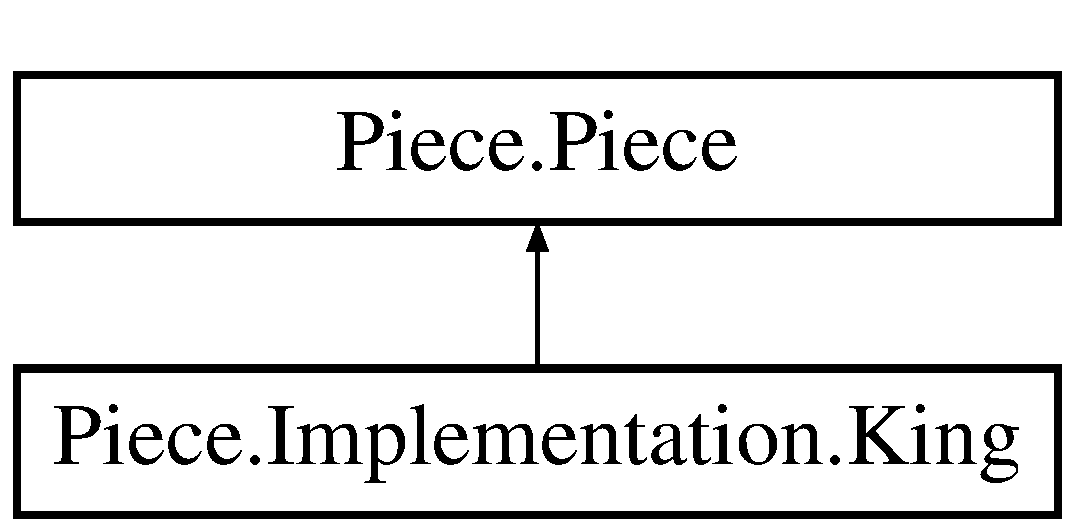
\includegraphics[height=2.000000cm]{classPiece_1_1Implementation_1_1King}
\end{center}
\end{figure}
\subsection*{Public Member Functions}
\begin{DoxyCompactItemize}
\item 
\hyperlink{classPiece_1_1Implementation_1_1King_a644208ee48f86c9da6fc27959fb3ef2a}{King} (\hyperlink{classUtil_1_1Position}{Position} start\-Position, int assign\-User\-Id, int assign\-Piece\-Id)  throws Exception 
\end{DoxyCompactItemize}
\subsection*{Protected Member Functions}
\begin{DoxyCompactItemize}
\item 
void \hyperlink{classPiece_1_1Implementation_1_1King_a3c191fbeb257c92630fb48813677b9c8}{init\-Directions} ()  throws Exception 
\end{DoxyCompactItemize}
\subsection*{Additional Inherited Members}


\subsection{Detailed Description}
Class that defines the \hyperlink{classPiece_1_1Implementation_1_1King}{King} chess piece \begin{DoxyAuthor}{Author}
Taccio Yamamoto 
\end{DoxyAuthor}


\subsection{Constructor \& Destructor Documentation}
\hypertarget{classPiece_1_1Implementation_1_1King_a644208ee48f86c9da6fc27959fb3ef2a}{\index{Piece\-::\-Implementation\-::\-King@{Piece\-::\-Implementation\-::\-King}!King@{King}}
\index{King@{King}!Piece::Implementation::King@{Piece\-::\-Implementation\-::\-King}}
\subsubsection[{King}]{\setlength{\rightskip}{0pt plus 5cm}Piece.\-Implementation.\-King.\-King (
\begin{DoxyParamCaption}
\item[{{\bf Position}}]{start\-Position, }
\item[{int}]{assign\-User\-Id, }
\item[{int}]{assign\-Piece\-Id}
\end{DoxyParamCaption}
)  throws Exception \hspace{0.3cm}{\ttfamily [inline]}}}\label{classPiece_1_1Implementation_1_1King_a644208ee48f86c9da6fc27959fb3ef2a}
Constructor 
\begin{DoxyParams}{Parameters}
{\em start\-Position} & -\/ start position of the piece \\
\hline
{\em assign\-User\-Id} & -\/ user identification of the owner of the piece \\
\hline
{\em assign\-Piece\-Id} & -\/ unique id assigned to the piece \\
\hline
\end{DoxyParams}

\begin{DoxyExceptions}{Exceptions}
{\em Exception} & throws possible exceptions from the init\-Directions function \\
\hline
\end{DoxyExceptions}


\subsection{Member Function Documentation}
\hypertarget{classPiece_1_1Implementation_1_1King_a3c191fbeb257c92630fb48813677b9c8}{\index{Piece\-::\-Implementation\-::\-King@{Piece\-::\-Implementation\-::\-King}!init\-Directions@{init\-Directions}}
\index{init\-Directions@{init\-Directions}!Piece::Implementation::King@{Piece\-::\-Implementation\-::\-King}}
\subsubsection[{init\-Directions}]{\setlength{\rightskip}{0pt plus 5cm}void Piece.\-Implementation.\-King.\-init\-Directions (
\begin{DoxyParamCaption}
{}
\end{DoxyParamCaption}
)  throws Exception \hspace{0.3cm}{\ttfamily [inline]}, {\ttfamily [protected]}, {\ttfamily [virtual]}}}\label{classPiece_1_1Implementation_1_1King_a3c191fbeb257c92630fb48813677b9c8}
Initializes the legal directions of the piece 
\begin{DoxyExceptions}{Exceptions}
{\em Exception} & throws exceptions from the Direction constructor \\
\hline
\end{DoxyExceptions}


Implements \hyperlink{classPiece_1_1Piece_af8bf9c4edb5bd73c91f3f8b21793ca5b}{Piece.\-Piece}.



The documentation for this class was generated from the following file\-:\begin{DoxyCompactItemize}
\item 
src/\-Piece/\-Implementation/King.\-java\end{DoxyCompactItemize}

\hypertarget{classPiece_1_1Implementation_1_1KingTest}{\section{Piece.\-Implementation.\-King\-Test Class Reference}
\label{classPiece_1_1Implementation_1_1KingTest}\index{Piece.\-Implementation.\-King\-Test@{Piece.\-Implementation.\-King\-Test}}
}
\subsection*{Public Member Functions}
\begin{DoxyCompactItemize}
\item 
void \hyperlink{classPiece_1_1Implementation_1_1KingTest_a22f09584c054283dda9d38323edb8700}{set\-Up} ()  throws Exception 
\item 
\hypertarget{classPiece_1_1Implementation_1_1KingTest_a73c625357616ccb229967e8a02e6d7ce}{void {\bfseries test\-Piece\-Type} ()}\label{classPiece_1_1Implementation_1_1KingTest_a73c625357616ccb229967e8a02e6d7ce}

\item 
\hypertarget{classPiece_1_1Implementation_1_1KingTest_a9f8b42cc4c08d715cf92dd6494d16c37}{void {\bfseries test\-Can\-Move} ()  throws Exception}\label{classPiece_1_1Implementation_1_1KingTest_a9f8b42cc4c08d715cf92dd6494d16c37}

\item 
\hypertarget{classPiece_1_1Implementation_1_1KingTest_ae340bfe3b9bcba957edd108ecf519c9e}{void {\bfseries test\-Move} ()  throws Exception}\label{classPiece_1_1Implementation_1_1KingTest_ae340bfe3b9bcba957edd108ecf519c9e}

\item 
\hypertarget{classPiece_1_1Implementation_1_1KingTest_ab7c93313959595737056c7aef04c535e}{void {\bfseries test\-Get\-Functions} ()}\label{classPiece_1_1Implementation_1_1KingTest_ab7c93313959595737056c7aef04c535e}

\end{DoxyCompactItemize}


\subsection{Detailed Description}
Created by taccio on 2/14/17. 

\subsection{Member Function Documentation}
\hypertarget{classPiece_1_1Implementation_1_1KingTest_a22f09584c054283dda9d38323edb8700}{\index{Piece\-::\-Implementation\-::\-King\-Test@{Piece\-::\-Implementation\-::\-King\-Test}!set\-Up@{set\-Up}}
\index{set\-Up@{set\-Up}!Piece::Implementation::KingTest@{Piece\-::\-Implementation\-::\-King\-Test}}
\subsubsection[{set\-Up}]{\setlength{\rightskip}{0pt plus 5cm}void Piece.\-Implementation.\-King\-Test.\-set\-Up (
\begin{DoxyParamCaption}
{}
\end{DoxyParamCaption}
)  throws Exception \hspace{0.3cm}{\ttfamily [inline]}}}\label{classPiece_1_1Implementation_1_1KingTest_a22f09584c054283dda9d38323edb8700}
Calls setup function before every test function 
\begin{DoxyExceptions}{Exceptions}
{\em Exception} & \\
\hline
\end{DoxyExceptions}


The documentation for this class was generated from the following file\-:\begin{DoxyCompactItemize}
\item 
test/\-Piece/\-Implementation/King\-Test.\-java\end{DoxyCompactItemize}

\hypertarget{classPiece_1_1Implementation_1_1Knight}{\section{Piece.\-Implementation.\-Knight Class Reference}
\label{classPiece_1_1Implementation_1_1Knight}\index{Piece.\-Implementation.\-Knight@{Piece.\-Implementation.\-Knight}}
}
Inheritance diagram for Piece.\-Implementation.\-Knight\-:\begin{figure}[H]
\begin{center}
\leavevmode
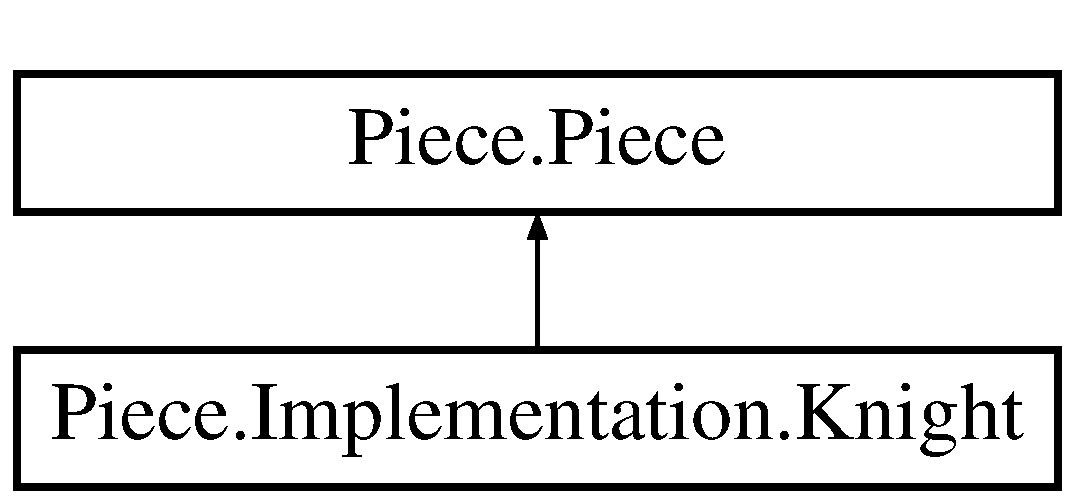
\includegraphics[height=2.000000cm]{classPiece_1_1Implementation_1_1Knight}
\end{center}
\end{figure}
\subsection*{Public Member Functions}
\begin{DoxyCompactItemize}
\item 
\hyperlink{classPiece_1_1Implementation_1_1Knight_a030cb62a535ccf809b9bb4c6f6a10daa}{Knight} (\hyperlink{classUtil_1_1Position}{Position} start\-Position, int assign\-User\-Id, int assign\-Piece\-Id)  throws Exception 
\end{DoxyCompactItemize}
\subsection*{Protected Member Functions}
\begin{DoxyCompactItemize}
\item 
void \hyperlink{classPiece_1_1Implementation_1_1Knight_a06194dc37dbf065c81f6432a4ea18103}{init\-Directions} ()  throws Exception 
\end{DoxyCompactItemize}
\subsection*{Additional Inherited Members}


\subsection{Detailed Description}
Class that defines the \hyperlink{classPiece_1_1Implementation_1_1Knight}{Knight} chess piece \begin{DoxyAuthor}{Author}
Taccio Yamamoto 
\end{DoxyAuthor}


\subsection{Constructor \& Destructor Documentation}
\hypertarget{classPiece_1_1Implementation_1_1Knight_a030cb62a535ccf809b9bb4c6f6a10daa}{\index{Piece\-::\-Implementation\-::\-Knight@{Piece\-::\-Implementation\-::\-Knight}!Knight@{Knight}}
\index{Knight@{Knight}!Piece::Implementation::Knight@{Piece\-::\-Implementation\-::\-Knight}}
\subsubsection[{Knight}]{\setlength{\rightskip}{0pt plus 5cm}Piece.\-Implementation.\-Knight.\-Knight (
\begin{DoxyParamCaption}
\item[{{\bf Position}}]{start\-Position, }
\item[{int}]{assign\-User\-Id, }
\item[{int}]{assign\-Piece\-Id}
\end{DoxyParamCaption}
)  throws Exception \hspace{0.3cm}{\ttfamily [inline]}}}\label{classPiece_1_1Implementation_1_1Knight_a030cb62a535ccf809b9bb4c6f6a10daa}
Constructor 
\begin{DoxyParams}{Parameters}
{\em start\-Position} & -\/ start position of the piece \\
\hline
{\em assign\-User\-Id} & -\/ user identification of the owner of the piece \\
\hline
{\em assign\-Piece\-Id} & -\/ unique id assigned to the piece \\
\hline
\end{DoxyParams}

\begin{DoxyExceptions}{Exceptions}
{\em Exception} & throws possible exceptions from the init\-Directions function \\
\hline
\end{DoxyExceptions}


\subsection{Member Function Documentation}
\hypertarget{classPiece_1_1Implementation_1_1Knight_a06194dc37dbf065c81f6432a4ea18103}{\index{Piece\-::\-Implementation\-::\-Knight@{Piece\-::\-Implementation\-::\-Knight}!init\-Directions@{init\-Directions}}
\index{init\-Directions@{init\-Directions}!Piece::Implementation::Knight@{Piece\-::\-Implementation\-::\-Knight}}
\subsubsection[{init\-Directions}]{\setlength{\rightskip}{0pt plus 5cm}void Piece.\-Implementation.\-Knight.\-init\-Directions (
\begin{DoxyParamCaption}
{}
\end{DoxyParamCaption}
)  throws Exception \hspace{0.3cm}{\ttfamily [inline]}, {\ttfamily [protected]}, {\ttfamily [virtual]}}}\label{classPiece_1_1Implementation_1_1Knight_a06194dc37dbf065c81f6432a4ea18103}
Initializes the legal directions of the piece 
\begin{DoxyExceptions}{Exceptions}
{\em Exception} & throws exceptions from the Direction constructor \\
\hline
\end{DoxyExceptions}


Implements \hyperlink{classPiece_1_1Piece_af8bf9c4edb5bd73c91f3f8b21793ca5b}{Piece.\-Piece}.



The documentation for this class was generated from the following file\-:\begin{DoxyCompactItemize}
\item 
src/\-Piece/\-Implementation/Knight.\-java\end{DoxyCompactItemize}

\hypertarget{classPiece_1_1Implementation_1_1KnightTest}{\section{Piece.\-Implementation.\-Knight\-Test Class Reference}
\label{classPiece_1_1Implementation_1_1KnightTest}\index{Piece.\-Implementation.\-Knight\-Test@{Piece.\-Implementation.\-Knight\-Test}}
}
\subsection*{Public Member Functions}
\begin{DoxyCompactItemize}
\item 
void \hyperlink{classPiece_1_1Implementation_1_1KnightTest_a08efc9f0f3fdd9e9a2d0f7d9b6707780}{set\-Up} ()  throws Exception 
\item 
\hypertarget{classPiece_1_1Implementation_1_1KnightTest_afddaa01647df0e6fbd19f2ca2510d248}{void {\bfseries test\-Piece\-Type} ()}\label{classPiece_1_1Implementation_1_1KnightTest_afddaa01647df0e6fbd19f2ca2510d248}

\item 
\hypertarget{classPiece_1_1Implementation_1_1KnightTest_a1765952fb19187d8851d505073ec6ef1}{void {\bfseries test\-Can\-Move} ()  throws Exception}\label{classPiece_1_1Implementation_1_1KnightTest_a1765952fb19187d8851d505073ec6ef1}

\item 
\hypertarget{classPiece_1_1Implementation_1_1KnightTest_a1416907f4eac35538b6e08a5df81fc38}{void {\bfseries test\-Move} ()  throws Exception}\label{classPiece_1_1Implementation_1_1KnightTest_a1416907f4eac35538b6e08a5df81fc38}

\item 
\hypertarget{classPiece_1_1Implementation_1_1KnightTest_ae893bc2aefe761c09bf7e6c369f472cd}{void {\bfseries test\-Get\-Functions} ()}\label{classPiece_1_1Implementation_1_1KnightTest_ae893bc2aefe761c09bf7e6c369f472cd}

\end{DoxyCompactItemize}


\subsection{Detailed Description}
Created by taccio on 2/13/17. 

\subsection{Member Function Documentation}
\hypertarget{classPiece_1_1Implementation_1_1KnightTest_a08efc9f0f3fdd9e9a2d0f7d9b6707780}{\index{Piece\-::\-Implementation\-::\-Knight\-Test@{Piece\-::\-Implementation\-::\-Knight\-Test}!set\-Up@{set\-Up}}
\index{set\-Up@{set\-Up}!Piece::Implementation::KnightTest@{Piece\-::\-Implementation\-::\-Knight\-Test}}
\subsubsection[{set\-Up}]{\setlength{\rightskip}{0pt plus 5cm}void Piece.\-Implementation.\-Knight\-Test.\-set\-Up (
\begin{DoxyParamCaption}
{}
\end{DoxyParamCaption}
)  throws Exception \hspace{0.3cm}{\ttfamily [inline]}}}\label{classPiece_1_1Implementation_1_1KnightTest_a08efc9f0f3fdd9e9a2d0f7d9b6707780}
Calls setup function before every test function 
\begin{DoxyExceptions}{Exceptions}
{\em Exception} & \\
\hline
\end{DoxyExceptions}


The documentation for this class was generated from the following file\-:\begin{DoxyCompactItemize}
\item 
test/\-Piece/\-Implementation/Knight\-Test.\-java\end{DoxyCompactItemize}

\hypertarget{classPiece_1_1Implementation_1_1Pawn}{\section{Piece.\-Implementation.\-Pawn Class Reference}
\label{classPiece_1_1Implementation_1_1Pawn}\index{Piece.\-Implementation.\-Pawn@{Piece.\-Implementation.\-Pawn}}
}
Inheritance diagram for Piece.\-Implementation.\-Pawn\-:\begin{figure}[H]
\begin{center}
\leavevmode
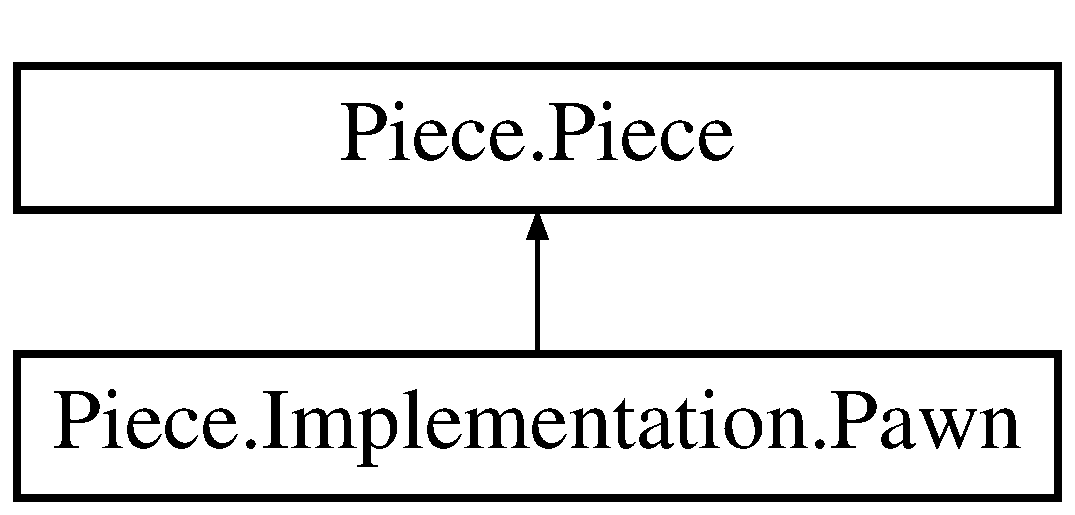
\includegraphics[height=2.000000cm]{classPiece_1_1Implementation_1_1Pawn}
\end{center}
\end{figure}
\subsection*{Public Member Functions}
\begin{DoxyCompactItemize}
\item 
\hyperlink{classPiece_1_1Implementation_1_1Pawn_aa8ed50a38f542bedfbb2b593ec8d28e7}{Pawn} (\hyperlink{classUtil_1_1Position}{Position} start\-Position, int assign\-User\-Id, int assign\-Piece\-Id)  throws Exception 
\item 
boolean \hyperlink{classPiece_1_1Implementation_1_1Pawn_a81011c0564bcf4d1931eb0e11eb7d7e8}{move} (\hyperlink{classUtil_1_1Position}{Position} new\-Position, \hyperlink{classBoard_1_1Board}{Board} board)  throws Exception 
\item 
boolean \hyperlink{classPiece_1_1Implementation_1_1Pawn_aaf6b3635a8fa5c0243223dbc065c4ad3}{can\-Move} (\hyperlink{classUtil_1_1Position}{Position} new\-Position, \hyperlink{classBoard_1_1Board}{Board} board)  throws Exception 
\end{DoxyCompactItemize}
\subsection*{Protected Member Functions}
\begin{DoxyCompactItemize}
\item 
void \hyperlink{classPiece_1_1Implementation_1_1Pawn_abe53393d31e868047a99adc17ffe50f6}{init\-Directions} ()
\end{DoxyCompactItemize}
\subsection*{Additional Inherited Members}


\subsection{Detailed Description}
Class that defines the \hyperlink{classPiece_1_1Implementation_1_1Pawn}{Pawn} chess piece \begin{DoxyAuthor}{Author}
Taccio Yamamoto 
\end{DoxyAuthor}


\subsection{Constructor \& Destructor Documentation}
\hypertarget{classPiece_1_1Implementation_1_1Pawn_aa8ed50a38f542bedfbb2b593ec8d28e7}{\index{Piece\-::\-Implementation\-::\-Pawn@{Piece\-::\-Implementation\-::\-Pawn}!Pawn@{Pawn}}
\index{Pawn@{Pawn}!Piece::Implementation::Pawn@{Piece\-::\-Implementation\-::\-Pawn}}
\subsubsection[{Pawn}]{\setlength{\rightskip}{0pt plus 5cm}Piece.\-Implementation.\-Pawn.\-Pawn (
\begin{DoxyParamCaption}
\item[{{\bf Position}}]{start\-Position, }
\item[{int}]{assign\-User\-Id, }
\item[{int}]{assign\-Piece\-Id}
\end{DoxyParamCaption}
)  throws Exception \hspace{0.3cm}{\ttfamily [inline]}}}\label{classPiece_1_1Implementation_1_1Pawn_aa8ed50a38f542bedfbb2b593ec8d28e7}
Constructor 
\begin{DoxyParams}{Parameters}
{\em start\-Position} & -\/ start position of the piece \\
\hline
{\em assign\-User\-Id} & -\/ user identification of the owner of the piece \\
\hline
{\em assign\-Piece\-Id} & -\/ unique id assigned to the piece \\
\hline
\end{DoxyParams}

\begin{DoxyExceptions}{Exceptions}
{\em Exception} & throws possible exceptions from the init\-Directions function \\
\hline
\end{DoxyExceptions}


\subsection{Member Function Documentation}
\hypertarget{classPiece_1_1Implementation_1_1Pawn_aaf6b3635a8fa5c0243223dbc065c4ad3}{\index{Piece\-::\-Implementation\-::\-Pawn@{Piece\-::\-Implementation\-::\-Pawn}!can\-Move@{can\-Move}}
\index{can\-Move@{can\-Move}!Piece::Implementation::Pawn@{Piece\-::\-Implementation\-::\-Pawn}}
\subsubsection[{can\-Move}]{\setlength{\rightskip}{0pt plus 5cm}boolean Piece.\-Implementation.\-Pawn.\-can\-Move (
\begin{DoxyParamCaption}
\item[{{\bf Position}}]{new\-Position, }
\item[{{\bf Board}}]{board}
\end{DoxyParamCaption}
)  throws Exception \hspace{0.3cm}{\ttfamily [inline]}}}\label{classPiece_1_1Implementation_1_1Pawn_aaf6b3635a8fa5c0243223dbc065c4ad3}
Checks if the piece can move to the new\-Position. This function overrides the can\-Move \hyperlink{classPiece_1_1Piece}{Piece} function 
\begin{DoxyParams}{Parameters}
{\em new\-Position} & -\/ tentative position to set piece \\
\hline
{\em board} & -\/ board that keeps track of all the pieces \\
\hline
\end{DoxyParams}
\begin{DoxyReturn}{Returns}
true if the piece can move to the new\-Position 
\end{DoxyReturn}

\begin{DoxyExceptions}{Exceptions}
{\em Exception} & throws possible exception from the board.\-get\-Piece() function \\
\hline
\end{DoxyExceptions}
\hypertarget{classPiece_1_1Implementation_1_1Pawn_abe53393d31e868047a99adc17ffe50f6}{\index{Piece\-::\-Implementation\-::\-Pawn@{Piece\-::\-Implementation\-::\-Pawn}!init\-Directions@{init\-Directions}}
\index{init\-Directions@{init\-Directions}!Piece::Implementation::Pawn@{Piece\-::\-Implementation\-::\-Pawn}}
\subsubsection[{init\-Directions}]{\setlength{\rightskip}{0pt plus 5cm}void Piece.\-Implementation.\-Pawn.\-init\-Directions (
\begin{DoxyParamCaption}
{}
\end{DoxyParamCaption}
)\hspace{0.3cm}{\ttfamily [inline]}, {\ttfamily [protected]}, {\ttfamily [virtual]}}}\label{classPiece_1_1Implementation_1_1Pawn_abe53393d31e868047a99adc17ffe50f6}
Initializes the legal directions of the piece 
\begin{DoxyExceptions}{Exceptions}
{\em Exception} & throws exceptions from the Direction constructor \\
\hline
\end{DoxyExceptions}


Implements \hyperlink{classPiece_1_1Piece_af8bf9c4edb5bd73c91f3f8b21793ca5b}{Piece.\-Piece}.

\hypertarget{classPiece_1_1Implementation_1_1Pawn_a81011c0564bcf4d1931eb0e11eb7d7e8}{\index{Piece\-::\-Implementation\-::\-Pawn@{Piece\-::\-Implementation\-::\-Pawn}!move@{move}}
\index{move@{move}!Piece::Implementation::Pawn@{Piece\-::\-Implementation\-::\-Pawn}}
\subsubsection[{move}]{\setlength{\rightskip}{0pt plus 5cm}boolean Piece.\-Implementation.\-Pawn.\-move (
\begin{DoxyParamCaption}
\item[{{\bf Position}}]{new\-Position, }
\item[{{\bf Board}}]{board}
\end{DoxyParamCaption}
)  throws Exception \hspace{0.3cm}{\ttfamily [inline]}}}\label{classPiece_1_1Implementation_1_1Pawn_a81011c0564bcf4d1931eb0e11eb7d7e8}
Overrides the move function to move a piece object to the new\-Position.  new\-Position -\/ tentative position to set piece  board -\/ board that keeps track of all the pieces \begin{DoxyReturn}{Returns}
true if the piece was successfully able to be moved 
\end{DoxyReturn}

\begin{DoxyExceptions}{Exceptions}
{\em Exception} & from the helper functions that checks different possible positions \\
\hline
\end{DoxyExceptions}


The documentation for this class was generated from the following file\-:\begin{DoxyCompactItemize}
\item 
src/\-Piece/\-Implementation/Pawn.\-java\end{DoxyCompactItemize}

\hypertarget{classPiece_1_1Implementation_1_1PawnTest}{\section{Piece.\-Implementation.\-Pawn\-Test Class Reference}
\label{classPiece_1_1Implementation_1_1PawnTest}\index{Piece.\-Implementation.\-Pawn\-Test@{Piece.\-Implementation.\-Pawn\-Test}}
}
\subsection*{Public Member Functions}
\begin{DoxyCompactItemize}
\item 
void \hyperlink{classPiece_1_1Implementation_1_1PawnTest_ae274f39090097cc60c4f861bf2fe1a22}{set\-Up} ()  throws Exception 
\item 
\hypertarget{classPiece_1_1Implementation_1_1PawnTest_a6ecd01eb2d9f9eb6d97d17652a519582}{void {\bfseries test\-Piece\-Type} ()}\label{classPiece_1_1Implementation_1_1PawnTest_a6ecd01eb2d9f9eb6d97d17652a519582}

\item 
\hypertarget{classPiece_1_1Implementation_1_1PawnTest_a19660e5dff24a52ff4951218aafd3202}{void {\bfseries test\-Can\-Move} ()  throws Exception}\label{classPiece_1_1Implementation_1_1PawnTest_a19660e5dff24a52ff4951218aafd3202}

\item 
\hypertarget{classPiece_1_1Implementation_1_1PawnTest_a09de68d6a36f556f619649962a8900be}{void {\bfseries test\-Move} ()  throws Exception}\label{classPiece_1_1Implementation_1_1PawnTest_a09de68d6a36f556f619649962a8900be}

\item 
\hypertarget{classPiece_1_1Implementation_1_1PawnTest_ab8772a206d20ae1b400a913c36d615e9}{void {\bfseries test\-Get\-Functions} ()}\label{classPiece_1_1Implementation_1_1PawnTest_ab8772a206d20ae1b400a913c36d615e9}

\end{DoxyCompactItemize}


\subsection{Detailed Description}
Created by taccio on 2/7/17. 

\subsection{Member Function Documentation}
\hypertarget{classPiece_1_1Implementation_1_1PawnTest_ae274f39090097cc60c4f861bf2fe1a22}{\index{Piece\-::\-Implementation\-::\-Pawn\-Test@{Piece\-::\-Implementation\-::\-Pawn\-Test}!set\-Up@{set\-Up}}
\index{set\-Up@{set\-Up}!Piece::Implementation::PawnTest@{Piece\-::\-Implementation\-::\-Pawn\-Test}}
\subsubsection[{set\-Up}]{\setlength{\rightskip}{0pt plus 5cm}void Piece.\-Implementation.\-Pawn\-Test.\-set\-Up (
\begin{DoxyParamCaption}
{}
\end{DoxyParamCaption}
)  throws Exception \hspace{0.3cm}{\ttfamily [inline]}}}\label{classPiece_1_1Implementation_1_1PawnTest_ae274f39090097cc60c4f861bf2fe1a22}
Calls setup function before every test function 
\begin{DoxyExceptions}{Exceptions}
{\em Exception} & \\
\hline
\end{DoxyExceptions}


The documentation for this class was generated from the following file\-:\begin{DoxyCompactItemize}
\item 
test/\-Piece/\-Implementation/Pawn\-Test.\-java\end{DoxyCompactItemize}

\hypertarget{classPiece_1_1Piece}{\section{Piece.\-Piece Class Reference}
\label{classPiece_1_1Piece}\index{Piece.\-Piece@{Piece.\-Piece}}
}
Inheritance diagram for Piece.\-Piece\-:\begin{figure}[H]
\begin{center}
\leavevmode
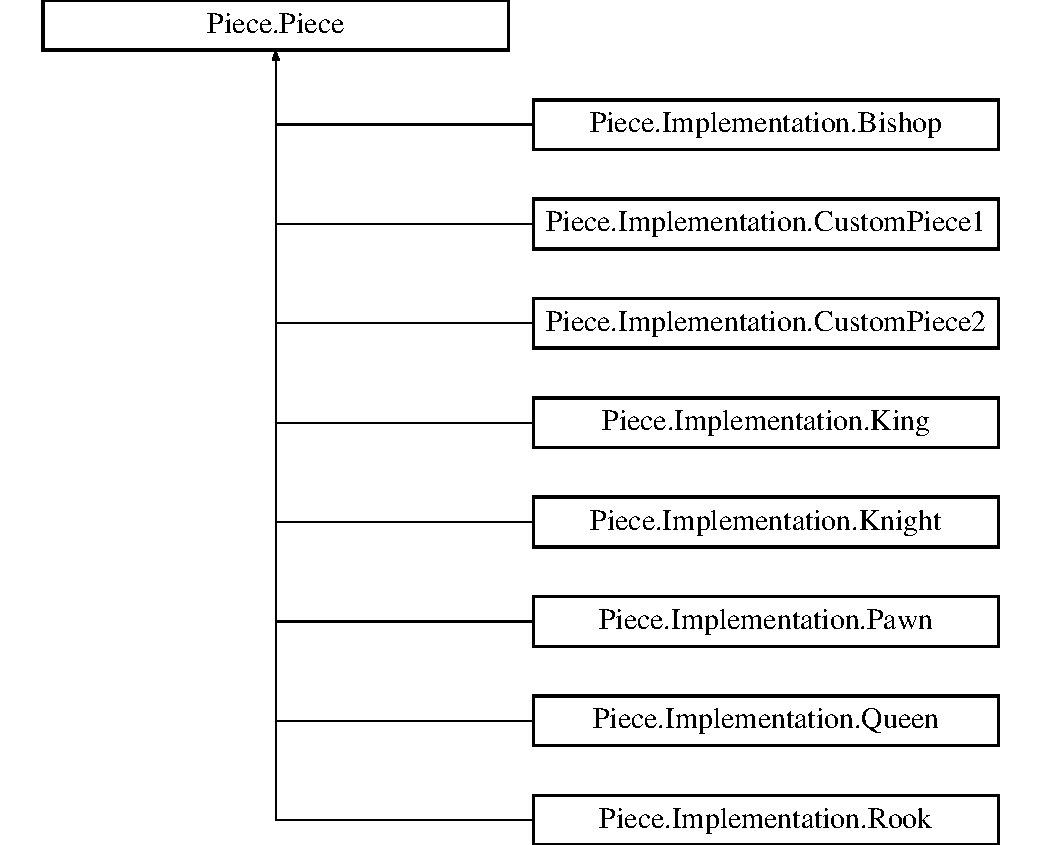
\includegraphics[height=12.000000cm]{classPiece_1_1Piece}
\end{center}
\end{figure}
\subsection*{Public Member Functions}
\begin{DoxyCompactItemize}
\item 
\hyperlink{classPiece_1_1Piece_a997635ad14cc0eb5d3df1b998d05df1d}{Piece} (\hyperlink{classUtil_1_1Position}{Position} start\-Position, int assign\-User\-Id, int assign\-Piece\-Id)  throws Exception 
\item 
\hyperlink{enumPiece_1_1PieceType}{Piece\-Type} \hyperlink{classPiece_1_1Piece_abe02eb4013ec562dfad1056245088add}{get\-Piece\-Type} ()
\item 
boolean \hyperlink{classPiece_1_1Piece_a472ffe2c12ba2a9d2d4a73e38c3f8d7f}{remove\-Direction} (\hyperlink{classUtil_1_1Direction}{Direction} rem\-Direction)
\item 
void \hyperlink{classPiece_1_1Piece_ab292128370c9df7d112cc7972bb8b1d0}{add\-Direction} (\hyperlink{classUtil_1_1Direction}{Direction} new\-Direction)
\item 
\hyperlink{classUtil_1_1Direction}{Direction} \hyperlink{classPiece_1_1Piece_a4068d2bdf5c732c0eee560df93cea966}{get\-Direction} (\hyperlink{classUtil_1_1Position}{Position} target\-Position)  throws Exception 
\item 
Array\-List$<$ \hyperlink{classUtil_1_1Direction}{Direction} $>$ \hyperlink{classPiece_1_1Piece_aee0dc72aed56d9a5c9612d3a9d545672}{get\-All\-Directions} ()
\item 
boolean \hyperlink{classPiece_1_1Piece_a23a749e9ef159a908cb66ddf8575b4a6}{move} (\hyperlink{classUtil_1_1Position}{Position} new\-Position, \hyperlink{classBoard_1_1Board}{Board} board)  throws Exception 
\item 
boolean \hyperlink{classPiece_1_1Piece_ad6d3c365ebdbee1c5a128d5cb645a5c3}{can\-Move} (\hyperlink{classUtil_1_1Position}{Position} new\-Position, \hyperlink{classBoard_1_1Board}{Board} board)  throws Exception 
\item 
int \hyperlink{classPiece_1_1Piece_a39912c2af6e604892dc897105aa511eb}{get\-User\-Id} ()
\item 
int \hyperlink{classPiece_1_1Piece_abb5dd621ae9e76e2aa622a67bf6219b0}{get\-Piece\-Id} ()
\item 
\hyperlink{classUtil_1_1Position}{Position} \hyperlink{classPiece_1_1Piece_a1aa0fc5fa0e9f96c701f7d3b7145560e}{get\-Position} ()
\item 
\hyperlink{classPiece_1_1Piece_a997635ad14cc0eb5d3df1b998d05df1d}{Piece} (\hyperlink{classUtil_1_1Position}{Position} start\-Position, int assign\-User\-Id, int assign\-Piece\-Id)  throws Exception 
\item 
\hyperlink{enumPiece_1_1PieceType}{Piece\-Type} \hyperlink{classPiece_1_1Piece_abe02eb4013ec562dfad1056245088add}{get\-Piece\-Type} ()
\item 
boolean \hyperlink{classPiece_1_1Piece_a472ffe2c12ba2a9d2d4a73e38c3f8d7f}{remove\-Direction} (\hyperlink{classUtil_1_1Direction}{Direction} rem\-Direction)
\item 
void \hyperlink{classPiece_1_1Piece_ab292128370c9df7d112cc7972bb8b1d0}{add\-Direction} (\hyperlink{classUtil_1_1Direction}{Direction} new\-Direction)
\item 
\hyperlink{classUtil_1_1Direction}{Direction} \hyperlink{classPiece_1_1Piece_a4068d2bdf5c732c0eee560df93cea966}{get\-Direction} (\hyperlink{classUtil_1_1Position}{Position} target\-Position)  throws Exception 
\item 
Array\-List$<$ \hyperlink{classUtil_1_1Direction}{Direction} $>$ \hyperlink{classPiece_1_1Piece_aee0dc72aed56d9a5c9612d3a9d545672}{get\-All\-Directions} ()
\item 
boolean \hyperlink{classPiece_1_1Piece_a23a749e9ef159a908cb66ddf8575b4a6}{move} (\hyperlink{classUtil_1_1Position}{Position} new\-Position, \hyperlink{classBoard_1_1Board}{Board} board)  throws Exception 
\item 
boolean \hyperlink{classPiece_1_1Piece_ad6d3c365ebdbee1c5a128d5cb645a5c3}{can\-Move} (\hyperlink{classUtil_1_1Position}{Position} new\-Position, \hyperlink{classBoard_1_1Board}{Board} board)  throws Exception 
\item 
int \hyperlink{classPiece_1_1Piece_a39912c2af6e604892dc897105aa511eb}{get\-User\-Id} ()
\item 
int \hyperlink{classPiece_1_1Piece_abb5dd621ae9e76e2aa622a67bf6219b0}{get\-Piece\-Id} ()
\item 
\hyperlink{classUtil_1_1Position}{Position} \hyperlink{classPiece_1_1Piece_a1aa0fc5fa0e9f96c701f7d3b7145560e}{get\-Position} ()
\end{DoxyCompactItemize}
\subsection*{Protected Member Functions}
\begin{DoxyCompactItemize}
\item 
abstract void \hyperlink{classPiece_1_1Piece_af8bf9c4edb5bd73c91f3f8b21793ca5b}{init\-Directions} ()  throws Exception
\item 
abstract void \hyperlink{classPiece_1_1Piece_af8bf9c4edb5bd73c91f3f8b21793ca5b}{init\-Directions} ()  throws Exception
\end{DoxyCompactItemize}
\subsection*{Protected Attributes}
\begin{DoxyCompactItemize}
\item 
\hypertarget{classPiece_1_1Piece_ac7ae9a6f1d238110c310de8f727c3979}{\hyperlink{enumPiece_1_1PieceType}{Piece\-Type} {\bfseries type}}\label{classPiece_1_1Piece_ac7ae9a6f1d238110c310de8f727c3979}

\item 
\hypertarget{classPiece_1_1Piece_a59d890b78035e87d7280094dd22a0ba3}{Array\-List$<$ \hyperlink{classUtil_1_1Direction}{Direction} $>$ {\bfseries directions}}\label{classPiece_1_1Piece_a59d890b78035e87d7280094dd22a0ba3}

\item 
\hypertarget{classPiece_1_1Piece_a8b64b4574722978ddec4659c5d481777}{\hyperlink{classUtil_1_1Position}{Position} {\bfseries position}}\label{classPiece_1_1Piece_a8b64b4574722978ddec4659c5d481777}

\item 
\hypertarget{classPiece_1_1Piece_ad8cf2bb72b487efd27d3ed55ae3dee72}{int {\bfseries user\-Id}}\label{classPiece_1_1Piece_ad8cf2bb72b487efd27d3ed55ae3dee72}

\item 
\hypertarget{classPiece_1_1Piece_acb50673ffa332035abd73052511bf883}{int {\bfseries piece\-Id}}\label{classPiece_1_1Piece_acb50673ffa332035abd73052511bf883}

\end{DoxyCompactItemize}


\subsection{Detailed Description}
The \hyperlink{classPiece_1_1Piece}{Piece} abstract class holds the basic framework to create other pieces. \begin{DoxyAuthor}{Author}
Taccio Yamamoto 
\end{DoxyAuthor}


\subsection{Constructor \& Destructor Documentation}
\hypertarget{classPiece_1_1Piece_a997635ad14cc0eb5d3df1b998d05df1d}{\index{Piece\-::\-Piece@{Piece\-::\-Piece}!Piece@{Piece}}
\index{Piece@{Piece}!Piece::Piece@{Piece\-::\-Piece}}
\subsubsection[{Piece}]{\setlength{\rightskip}{0pt plus 5cm}Piece.\-Piece.\-Piece (
\begin{DoxyParamCaption}
\item[{{\bf Position}}]{start\-Position, }
\item[{int}]{assign\-User\-Id, }
\item[{int}]{assign\-Piece\-Id}
\end{DoxyParamCaption}
)  throws Exception \hspace{0.3cm}{\ttfamily [inline]}}}\label{classPiece_1_1Piece_a997635ad14cc0eb5d3df1b998d05df1d}
\hyperlink{classPiece_1_1Piece}{Piece} constructor to initialize the position, user\-Id, and assign\-Piece\-Id of the piece  start\-Position -\/ initial \hyperlink{classPiece_1_1Piece}{Piece}'s position  assigned\-User\-Id -\/ id of the owner of the piece  assign\-Piece\-Id -\/ id of the specific piece 
\begin{DoxyExceptions}{Exceptions}
{\em Exception} & throws possible exceptions from the init\-Directions function \\
\hline
\end{DoxyExceptions}
\hypertarget{classPiece_1_1Piece_a997635ad14cc0eb5d3df1b998d05df1d}{\index{Piece\-::\-Piece@{Piece\-::\-Piece}!Piece@{Piece}}
\index{Piece@{Piece}!Piece::Piece@{Piece\-::\-Piece}}
\subsubsection[{Piece}]{\setlength{\rightskip}{0pt plus 5cm}Piece.\-Piece.\-Piece (
\begin{DoxyParamCaption}
\item[{{\bf Position}}]{start\-Position, }
\item[{int}]{assign\-User\-Id, }
\item[{int}]{assign\-Piece\-Id}
\end{DoxyParamCaption}
)  throws Exception \hspace{0.3cm}{\ttfamily [inline]}}}\label{classPiece_1_1Piece_a997635ad14cc0eb5d3df1b998d05df1d}
\hyperlink{classPiece_1_1Piece}{Piece} constructor to initialize the position, user\-Id, and assign\-Piece\-Id of the piece


\begin{DoxyExceptions}{Exceptions}
{\em Exception} & throws possible exceptions from the init\-Directions function  start\-Position -\/ initial \hyperlink{classPiece_1_1Piece}{Piece}'s position  assigned\-User\-Id -\/ id of the owner of the piece  assign\-Piece\-Id -\/ id of the specific piece \\
\hline
\end{DoxyExceptions}


\subsection{Member Function Documentation}
\hypertarget{classPiece_1_1Piece_ab292128370c9df7d112cc7972bb8b1d0}{\index{Piece\-::\-Piece@{Piece\-::\-Piece}!add\-Direction@{add\-Direction}}
\index{add\-Direction@{add\-Direction}!Piece::Piece@{Piece\-::\-Piece}}
\subsubsection[{add\-Direction}]{\setlength{\rightskip}{0pt plus 5cm}void Piece.\-Piece.\-add\-Direction (
\begin{DoxyParamCaption}
\item[{{\bf Direction}}]{new\-Direction}
\end{DoxyParamCaption}
)\hspace{0.3cm}{\ttfamily [inline]}}}\label{classPiece_1_1Piece_ab292128370c9df7d112cc7972bb8b1d0}
Adds a Direction object to the direction Arraylist 
\begin{DoxyParams}{Parameters}
{\em new\-Direction} & -\/ target direction to add \\
\hline
\end{DoxyParams}
\hypertarget{classPiece_1_1Piece_ab292128370c9df7d112cc7972bb8b1d0}{\index{Piece\-::\-Piece@{Piece\-::\-Piece}!add\-Direction@{add\-Direction}}
\index{add\-Direction@{add\-Direction}!Piece::Piece@{Piece\-::\-Piece}}
\subsubsection[{add\-Direction}]{\setlength{\rightskip}{0pt plus 5cm}void Piece.\-Piece.\-add\-Direction (
\begin{DoxyParamCaption}
\item[{{\bf Direction}}]{new\-Direction}
\end{DoxyParamCaption}
)\hspace{0.3cm}{\ttfamily [inline]}}}\label{classPiece_1_1Piece_ab292128370c9df7d112cc7972bb8b1d0}
Adds a Direction object to the direction Arraylist


\begin{DoxyParams}{Parameters}
{\em new\-Direction} & -\/ target direction to add \\
\hline
\end{DoxyParams}
\hypertarget{classPiece_1_1Piece_ad6d3c365ebdbee1c5a128d5cb645a5c3}{\index{Piece\-::\-Piece@{Piece\-::\-Piece}!can\-Move@{can\-Move}}
\index{can\-Move@{can\-Move}!Piece::Piece@{Piece\-::\-Piece}}
\subsubsection[{can\-Move}]{\setlength{\rightskip}{0pt plus 5cm}boolean Piece.\-Piece.\-can\-Move (
\begin{DoxyParamCaption}
\item[{{\bf Position}}]{new\-Position, }
\item[{{\bf Board}}]{board}
\end{DoxyParamCaption}
)  throws Exception \hspace{0.3cm}{\ttfamily [inline]}}}\label{classPiece_1_1Piece_ad6d3c365ebdbee1c5a128d5cb645a5c3}
Checks if the piece can move to the new\-Position 
\begin{DoxyParams}{Parameters}
{\em new\-Position} & -\/ tentative position to set piece \\
\hline
{\em board} & -\/ board that keeps track of all the pieces \\
\hline
\end{DoxyParams}
\begin{DoxyReturn}{Returns}
true if the piece can move to the new\-Position 
\end{DoxyReturn}

\begin{DoxyExceptions}{Exceptions}
{\em Exception} & throws possible exception from the board.\-get\-Piece() function \\
\hline
\end{DoxyExceptions}
\hypertarget{classPiece_1_1Piece_ad6d3c365ebdbee1c5a128d5cb645a5c3}{\index{Piece\-::\-Piece@{Piece\-::\-Piece}!can\-Move@{can\-Move}}
\index{can\-Move@{can\-Move}!Piece::Piece@{Piece\-::\-Piece}}
\subsubsection[{can\-Move}]{\setlength{\rightskip}{0pt plus 5cm}boolean Piece.\-Piece.\-can\-Move (
\begin{DoxyParamCaption}
\item[{{\bf Position}}]{new\-Position, }
\item[{{\bf Board}}]{board}
\end{DoxyParamCaption}
)  throws Exception \hspace{0.3cm}{\ttfamily [inline]}}}\label{classPiece_1_1Piece_ad6d3c365ebdbee1c5a128d5cb645a5c3}
Checks if the piece can move to the new\-Position


\begin{DoxyParams}{Parameters}
{\em new\-Position} & -\/ tentative position to set piece \\
\hline
{\em board} & -\/ board that keeps track of all the pieces \\
\hline
\end{DoxyParams}
\begin{DoxyReturn}{Returns}
true if the piece can move to the new\-Position 
\end{DoxyReturn}

\begin{DoxyExceptions}{Exceptions}
{\em Exception} & throws possible exception from the board.\-get\-Piece() function \\
\hline
\end{DoxyExceptions}
\hypertarget{classPiece_1_1Piece_aee0dc72aed56d9a5c9612d3a9d545672}{\index{Piece\-::\-Piece@{Piece\-::\-Piece}!get\-All\-Directions@{get\-All\-Directions}}
\index{get\-All\-Directions@{get\-All\-Directions}!Piece::Piece@{Piece\-::\-Piece}}
\subsubsection[{get\-All\-Directions}]{\setlength{\rightskip}{0pt plus 5cm}Array\-List$<${\bf Direction}$>$ Piece.\-Piece.\-get\-All\-Directions (
\begin{DoxyParamCaption}
{}
\end{DoxyParamCaption}
)\hspace{0.3cm}{\ttfamily [inline]}}}\label{classPiece_1_1Piece_aee0dc72aed56d9a5c9612d3a9d545672}
Returns the direction array list \begin{DoxyReturn}{Returns}
the direction array list 
\end{DoxyReturn}
\hypertarget{classPiece_1_1Piece_aee0dc72aed56d9a5c9612d3a9d545672}{\index{Piece\-::\-Piece@{Piece\-::\-Piece}!get\-All\-Directions@{get\-All\-Directions}}
\index{get\-All\-Directions@{get\-All\-Directions}!Piece::Piece@{Piece\-::\-Piece}}
\subsubsection[{get\-All\-Directions}]{\setlength{\rightskip}{0pt plus 5cm}Array\-List$<${\bf Direction}$>$ Piece.\-Piece.\-get\-All\-Directions (
\begin{DoxyParamCaption}
{}
\end{DoxyParamCaption}
)\hspace{0.3cm}{\ttfamily [inline]}}}\label{classPiece_1_1Piece_aee0dc72aed56d9a5c9612d3a9d545672}
Returns the direction array list

\begin{DoxyReturn}{Returns}
the direction array list 
\end{DoxyReturn}
\hypertarget{classPiece_1_1Piece_a4068d2bdf5c732c0eee560df93cea966}{\index{Piece\-::\-Piece@{Piece\-::\-Piece}!get\-Direction@{get\-Direction}}
\index{get\-Direction@{get\-Direction}!Piece::Piece@{Piece\-::\-Piece}}
\subsubsection[{get\-Direction}]{\setlength{\rightskip}{0pt plus 5cm}{\bf Direction} Piece.\-Piece.\-get\-Direction (
\begin{DoxyParamCaption}
\item[{{\bf Position}}]{target\-Position}
\end{DoxyParamCaption}
)  throws Exception \hspace{0.3cm}{\ttfamily [inline]}}}\label{classPiece_1_1Piece_a4068d2bdf5c732c0eee560df93cea966}
Returns direction from the piece to the target Position 
\begin{DoxyParams}{Parameters}
{\em target\-Position} & -\/ position to move to \\
\hline
\end{DoxyParams}
\begin{DoxyReturn}{Returns}
Direction object to the target position. If null, there is no direction to target position 
\end{DoxyReturn}
\hypertarget{classPiece_1_1Piece_a4068d2bdf5c732c0eee560df93cea966}{\index{Piece\-::\-Piece@{Piece\-::\-Piece}!get\-Direction@{get\-Direction}}
\index{get\-Direction@{get\-Direction}!Piece::Piece@{Piece\-::\-Piece}}
\subsubsection[{get\-Direction}]{\setlength{\rightskip}{0pt plus 5cm}{\bf Direction} Piece.\-Piece.\-get\-Direction (
\begin{DoxyParamCaption}
\item[{{\bf Position}}]{target\-Position}
\end{DoxyParamCaption}
)  throws Exception \hspace{0.3cm}{\ttfamily [inline]}}}\label{classPiece_1_1Piece_a4068d2bdf5c732c0eee560df93cea966}
Returns direction from the piece to the target Position


\begin{DoxyParams}{Parameters}
{\em target\-Position} & -\/ position to move to \\
\hline
\end{DoxyParams}
\begin{DoxyReturn}{Returns}
Direction object to the target position. If null, there is no direction to target position 
\end{DoxyReturn}
\hypertarget{classPiece_1_1Piece_abb5dd621ae9e76e2aa622a67bf6219b0}{\index{Piece\-::\-Piece@{Piece\-::\-Piece}!get\-Piece\-Id@{get\-Piece\-Id}}
\index{get\-Piece\-Id@{get\-Piece\-Id}!Piece::Piece@{Piece\-::\-Piece}}
\subsubsection[{get\-Piece\-Id}]{\setlength{\rightskip}{0pt plus 5cm}int Piece.\-Piece.\-get\-Piece\-Id (
\begin{DoxyParamCaption}
{}
\end{DoxyParamCaption}
)\hspace{0.3cm}{\ttfamily [inline]}}}\label{classPiece_1_1Piece_abb5dd621ae9e76e2aa622a67bf6219b0}
Get piece\-Id function \begin{DoxyReturn}{Returns}
piece\-Id to keep track of each unique piece 
\end{DoxyReturn}
\hypertarget{classPiece_1_1Piece_abb5dd621ae9e76e2aa622a67bf6219b0}{\index{Piece\-::\-Piece@{Piece\-::\-Piece}!get\-Piece\-Id@{get\-Piece\-Id}}
\index{get\-Piece\-Id@{get\-Piece\-Id}!Piece::Piece@{Piece\-::\-Piece}}
\subsubsection[{get\-Piece\-Id}]{\setlength{\rightskip}{0pt plus 5cm}int Piece.\-Piece.\-get\-Piece\-Id (
\begin{DoxyParamCaption}
{}
\end{DoxyParamCaption}
)\hspace{0.3cm}{\ttfamily [inline]}}}\label{classPiece_1_1Piece_abb5dd621ae9e76e2aa622a67bf6219b0}
Get piece\-Id function

\begin{DoxyReturn}{Returns}
piece\-Id to keep track of each unique piece 
\end{DoxyReturn}
\hypertarget{classPiece_1_1Piece_abe02eb4013ec562dfad1056245088add}{\index{Piece\-::\-Piece@{Piece\-::\-Piece}!get\-Piece\-Type@{get\-Piece\-Type}}
\index{get\-Piece\-Type@{get\-Piece\-Type}!Piece::Piece@{Piece\-::\-Piece}}
\subsubsection[{get\-Piece\-Type}]{\setlength{\rightskip}{0pt plus 5cm}{\bf Piece\-Type} Piece.\-Piece.\-get\-Piece\-Type (
\begin{DoxyParamCaption}
{}
\end{DoxyParamCaption}
)\hspace{0.3cm}{\ttfamily [inline]}}}\label{classPiece_1_1Piece_abe02eb4013ec562dfad1056245088add}
Gets the \hyperlink{enumPiece_1_1PieceType}{Piece\-Type} of the \hyperlink{classPiece_1_1Piece}{Piece} object \begin{DoxyReturn}{Returns}

\end{DoxyReturn}
\hypertarget{classPiece_1_1Piece_abe02eb4013ec562dfad1056245088add}{\index{Piece\-::\-Piece@{Piece\-::\-Piece}!get\-Piece\-Type@{get\-Piece\-Type}}
\index{get\-Piece\-Type@{get\-Piece\-Type}!Piece::Piece@{Piece\-::\-Piece}}
\subsubsection[{get\-Piece\-Type}]{\setlength{\rightskip}{0pt plus 5cm}{\bf Piece\-Type} Piece.\-Piece.\-get\-Piece\-Type (
\begin{DoxyParamCaption}
{}
\end{DoxyParamCaption}
)\hspace{0.3cm}{\ttfamily [inline]}}}\label{classPiece_1_1Piece_abe02eb4013ec562dfad1056245088add}
Gets the \hyperlink{enumPiece_1_1PieceType}{Piece\-Type} of the \hyperlink{classPiece_1_1Piece}{Piece} object

\begin{DoxyReturn}{Returns}

\end{DoxyReturn}
\hypertarget{classPiece_1_1Piece_a1aa0fc5fa0e9f96c701f7d3b7145560e}{\index{Piece\-::\-Piece@{Piece\-::\-Piece}!get\-Position@{get\-Position}}
\index{get\-Position@{get\-Position}!Piece::Piece@{Piece\-::\-Piece}}
\subsubsection[{get\-Position}]{\setlength{\rightskip}{0pt plus 5cm}{\bf Position} Piece.\-Piece.\-get\-Position (
\begin{DoxyParamCaption}
{}
\end{DoxyParamCaption}
)\hspace{0.3cm}{\ttfamily [inline]}}}\label{classPiece_1_1Piece_a1aa0fc5fa0e9f96c701f7d3b7145560e}
Get the position object \begin{DoxyReturn}{Returns}
the Position object 
\end{DoxyReturn}
\hypertarget{classPiece_1_1Piece_a1aa0fc5fa0e9f96c701f7d3b7145560e}{\index{Piece\-::\-Piece@{Piece\-::\-Piece}!get\-Position@{get\-Position}}
\index{get\-Position@{get\-Position}!Piece::Piece@{Piece\-::\-Piece}}
\subsubsection[{get\-Position}]{\setlength{\rightskip}{0pt plus 5cm}{\bf Position} Piece.\-Piece.\-get\-Position (
\begin{DoxyParamCaption}
{}
\end{DoxyParamCaption}
)\hspace{0.3cm}{\ttfamily [inline]}}}\label{classPiece_1_1Piece_a1aa0fc5fa0e9f96c701f7d3b7145560e}
Get the position object

\begin{DoxyReturn}{Returns}
the Position object 
\end{DoxyReturn}
\hypertarget{classPiece_1_1Piece_a39912c2af6e604892dc897105aa511eb}{\index{Piece\-::\-Piece@{Piece\-::\-Piece}!get\-User\-Id@{get\-User\-Id}}
\index{get\-User\-Id@{get\-User\-Id}!Piece::Piece@{Piece\-::\-Piece}}
\subsubsection[{get\-User\-Id}]{\setlength{\rightskip}{0pt plus 5cm}int Piece.\-Piece.\-get\-User\-Id (
\begin{DoxyParamCaption}
{}
\end{DoxyParamCaption}
)\hspace{0.3cm}{\ttfamily [inline]}}}\label{classPiece_1_1Piece_a39912c2af6e604892dc897105aa511eb}
Get user\-Id function \begin{DoxyReturn}{Returns}
user\-Id that keeps track of the owner of the piece 
\end{DoxyReturn}
\hypertarget{classPiece_1_1Piece_a39912c2af6e604892dc897105aa511eb}{\index{Piece\-::\-Piece@{Piece\-::\-Piece}!get\-User\-Id@{get\-User\-Id}}
\index{get\-User\-Id@{get\-User\-Id}!Piece::Piece@{Piece\-::\-Piece}}
\subsubsection[{get\-User\-Id}]{\setlength{\rightskip}{0pt plus 5cm}int Piece.\-Piece.\-get\-User\-Id (
\begin{DoxyParamCaption}
{}
\end{DoxyParamCaption}
)\hspace{0.3cm}{\ttfamily [inline]}}}\label{classPiece_1_1Piece_a39912c2af6e604892dc897105aa511eb}
Get user\-Id function

\begin{DoxyReturn}{Returns}
user\-Id that keeps track of the owner of the piece 
\end{DoxyReturn}
\hypertarget{classPiece_1_1Piece_af8bf9c4edb5bd73c91f3f8b21793ca5b}{\index{Piece\-::\-Piece@{Piece\-::\-Piece}!init\-Directions@{init\-Directions}}
\index{init\-Directions@{init\-Directions}!Piece::Piece@{Piece\-::\-Piece}}
\subsubsection[{init\-Directions}]{\setlength{\rightskip}{0pt plus 5cm}abstract void Piece.\-Piece.\-init\-Directions (
\begin{DoxyParamCaption}
{}
\end{DoxyParamCaption}
)  throws Exception\hspace{0.3cm}{\ttfamily [protected]}, {\ttfamily [pure virtual]}}}\label{classPiece_1_1Piece_af8bf9c4edb5bd73c91f3f8b21793ca5b}
Initializes the legal directions for the piece. Each inherited class should define the possible directions. 

Implemented in \hyperlink{classPiece_1_1Implementation_1_1Pawn_abe53393d31e868047a99adc17ffe50f6}{Piece.\-Implementation.\-Pawn}, \hyperlink{classPiece_1_1Implementation_1_1Pawn_abe53393d31e868047a99adc17ffe50f6}{Piece.\-Implementation.\-Pawn}, \hyperlink{classPiece_1_1Implementation_1_1Bishop_a86c4b94d2ab033427c12df9ad20b800f}{Piece.\-Implementation.\-Bishop}, \hyperlink{classPiece_1_1Implementation_1_1CustomPiece2_a33801c7e929e4ab100dd23c053c98dba}{Piece.\-Implementation.\-Custom\-Piece2}, \hyperlink{classPiece_1_1Implementation_1_1CustomPiece1_aa92e30cda4f19d89b622ec4bf2a6e78e}{Piece.\-Implementation.\-Custom\-Piece1}, \hyperlink{classPiece_1_1Implementation_1_1King_a3c191fbeb257c92630fb48813677b9c8}{Piece.\-Implementation.\-King}, \hyperlink{classPiece_1_1Implementation_1_1Knight_a06194dc37dbf065c81f6432a4ea18103}{Piece.\-Implementation.\-Knight}, \hyperlink{classPiece_1_1Implementation_1_1Queen_a0f7958e2d7f880df8f012b814dd83329}{Piece.\-Implementation.\-Queen}, \hyperlink{classPiece_1_1Implementation_1_1Rook_a0288b5ea743dcb4286fb0c91bd163f0d}{Piece.\-Implementation.\-Rook}, \hyperlink{classPiece_1_1Implementation_1_1Bishop_a86c4b94d2ab033427c12df9ad20b800f}{Piece.\-Implementation.\-Bishop}, \hyperlink{classPiece_1_1Implementation_1_1King_a3c191fbeb257c92630fb48813677b9c8}{Piece.\-Implementation.\-King}, \hyperlink{classPiece_1_1Implementation_1_1Knight_a06194dc37dbf065c81f6432a4ea18103}{Piece.\-Implementation.\-Knight}, \hyperlink{classPiece_1_1Implementation_1_1Queen_a0f7958e2d7f880df8f012b814dd83329}{Piece.\-Implementation.\-Queen}, and \hyperlink{classPiece_1_1Implementation_1_1Rook_a0288b5ea743dcb4286fb0c91bd163f0d}{Piece.\-Implementation.\-Rook}.

\hypertarget{classPiece_1_1Piece_af8bf9c4edb5bd73c91f3f8b21793ca5b}{\index{Piece\-::\-Piece@{Piece\-::\-Piece}!init\-Directions@{init\-Directions}}
\index{init\-Directions@{init\-Directions}!Piece::Piece@{Piece\-::\-Piece}}
\subsubsection[{init\-Directions}]{\setlength{\rightskip}{0pt plus 5cm}abstract void Piece.\-Piece.\-init\-Directions (
\begin{DoxyParamCaption}
{}
\end{DoxyParamCaption}
)  throws Exception\hspace{0.3cm}{\ttfamily [protected]}, {\ttfamily [pure virtual]}}}\label{classPiece_1_1Piece_af8bf9c4edb5bd73c91f3f8b21793ca5b}
Initializes the legal directions for the piece. Each inherited class should define the possible directions. 

Implemented in \hyperlink{classPiece_1_1Implementation_1_1Pawn_abe53393d31e868047a99adc17ffe50f6}{Piece.\-Implementation.\-Pawn}, \hyperlink{classPiece_1_1Implementation_1_1Pawn_abe53393d31e868047a99adc17ffe50f6}{Piece.\-Implementation.\-Pawn}, \hyperlink{classPiece_1_1Implementation_1_1Bishop_a86c4b94d2ab033427c12df9ad20b800f}{Piece.\-Implementation.\-Bishop}, \hyperlink{classPiece_1_1Implementation_1_1CustomPiece2_a33801c7e929e4ab100dd23c053c98dba}{Piece.\-Implementation.\-Custom\-Piece2}, \hyperlink{classPiece_1_1Implementation_1_1CustomPiece1_aa92e30cda4f19d89b622ec4bf2a6e78e}{Piece.\-Implementation.\-Custom\-Piece1}, \hyperlink{classPiece_1_1Implementation_1_1King_a3c191fbeb257c92630fb48813677b9c8}{Piece.\-Implementation.\-King}, \hyperlink{classPiece_1_1Implementation_1_1Knight_a06194dc37dbf065c81f6432a4ea18103}{Piece.\-Implementation.\-Knight}, \hyperlink{classPiece_1_1Implementation_1_1Queen_a0f7958e2d7f880df8f012b814dd83329}{Piece.\-Implementation.\-Queen}, \hyperlink{classPiece_1_1Implementation_1_1Rook_a0288b5ea743dcb4286fb0c91bd163f0d}{Piece.\-Implementation.\-Rook}, \hyperlink{classPiece_1_1Implementation_1_1Bishop_a86c4b94d2ab033427c12df9ad20b800f}{Piece.\-Implementation.\-Bishop}, \hyperlink{classPiece_1_1Implementation_1_1King_a3c191fbeb257c92630fb48813677b9c8}{Piece.\-Implementation.\-King}, \hyperlink{classPiece_1_1Implementation_1_1Knight_a06194dc37dbf065c81f6432a4ea18103}{Piece.\-Implementation.\-Knight}, \hyperlink{classPiece_1_1Implementation_1_1Queen_a0f7958e2d7f880df8f012b814dd83329}{Piece.\-Implementation.\-Queen}, and \hyperlink{classPiece_1_1Implementation_1_1Rook_a0288b5ea743dcb4286fb0c91bd163f0d}{Piece.\-Implementation.\-Rook}.

\hypertarget{classPiece_1_1Piece_a23a749e9ef159a908cb66ddf8575b4a6}{\index{Piece\-::\-Piece@{Piece\-::\-Piece}!move@{move}}
\index{move@{move}!Piece::Piece@{Piece\-::\-Piece}}
\subsubsection[{move}]{\setlength{\rightskip}{0pt plus 5cm}boolean Piece.\-Piece.\-move (
\begin{DoxyParamCaption}
\item[{{\bf Position}}]{new\-Position, }
\item[{{\bf Board}}]{board}
\end{DoxyParamCaption}
)  throws Exception \hspace{0.3cm}{\ttfamily [inline]}}}\label{classPiece_1_1Piece_a23a749e9ef159a908cb66ddf8575b4a6}
Moves the piece object to the new\-Position.  new\-Position -\/ tentative position to set piece  board -\/ board that keeps track of all the pieces \begin{DoxyReturn}{Returns}
true if the piece was successfully able to be moved 
\end{DoxyReturn}
\hypertarget{classPiece_1_1Piece_a23a749e9ef159a908cb66ddf8575b4a6}{\index{Piece\-::\-Piece@{Piece\-::\-Piece}!move@{move}}
\index{move@{move}!Piece::Piece@{Piece\-::\-Piece}}
\subsubsection[{move}]{\setlength{\rightskip}{0pt plus 5cm}boolean Piece.\-Piece.\-move (
\begin{DoxyParamCaption}
\item[{{\bf Position}}]{new\-Position, }
\item[{{\bf Board}}]{board}
\end{DoxyParamCaption}
)  throws Exception \hspace{0.3cm}{\ttfamily [inline]}}}\label{classPiece_1_1Piece_a23a749e9ef159a908cb66ddf8575b4a6}
Moves the piece object to the new\-Position.

\begin{DoxyReturn}{Returns}
true if the piece was successfully able to be moved  new\-Position -\/ tentative position to set piece  board -\/ board that keeps track of all the pieces 
\end{DoxyReturn}
\hypertarget{classPiece_1_1Piece_a472ffe2c12ba2a9d2d4a73e38c3f8d7f}{\index{Piece\-::\-Piece@{Piece\-::\-Piece}!remove\-Direction@{remove\-Direction}}
\index{remove\-Direction@{remove\-Direction}!Piece::Piece@{Piece\-::\-Piece}}
\subsubsection[{remove\-Direction}]{\setlength{\rightskip}{0pt plus 5cm}boolean Piece.\-Piece.\-remove\-Direction (
\begin{DoxyParamCaption}
\item[{{\bf Direction}}]{rem\-Direction}
\end{DoxyParamCaption}
)\hspace{0.3cm}{\ttfamily [inline]}}}\label{classPiece_1_1Piece_a472ffe2c12ba2a9d2d4a73e38c3f8d7f}
Removes Direction object from direction arraylist 
\begin{DoxyParams}{Parameters}
{\em rem\-Direction} & -\/ target direction to remove \\
\hline
\end{DoxyParams}
\begin{DoxyReturn}{Returns}
true if removed object from the list 
\end{DoxyReturn}
\hypertarget{classPiece_1_1Piece_a472ffe2c12ba2a9d2d4a73e38c3f8d7f}{\index{Piece\-::\-Piece@{Piece\-::\-Piece}!remove\-Direction@{remove\-Direction}}
\index{remove\-Direction@{remove\-Direction}!Piece::Piece@{Piece\-::\-Piece}}
\subsubsection[{remove\-Direction}]{\setlength{\rightskip}{0pt plus 5cm}boolean Piece.\-Piece.\-remove\-Direction (
\begin{DoxyParamCaption}
\item[{{\bf Direction}}]{rem\-Direction}
\end{DoxyParamCaption}
)\hspace{0.3cm}{\ttfamily [inline]}}}\label{classPiece_1_1Piece_a472ffe2c12ba2a9d2d4a73e38c3f8d7f}
Removes Direction object from direction arraylist


\begin{DoxyParams}{Parameters}
{\em rem\-Direction} & -\/ target direction to remove \\
\hline
\end{DoxyParams}
\begin{DoxyReturn}{Returns}
true if removed object from the list 
\end{DoxyReturn}


The documentation for this class was generated from the following files\-:\begin{DoxyCompactItemize}
\item 
Assignment1.\-0/src/\-Piece/Piece.\-java\item 
src/\-Piece/Piece.\-java\end{DoxyCompactItemize}

\hypertarget{enumPiece_1_1PieceType}{\section{Piece.\-Piece\-Type Enum Reference}
\label{enumPiece_1_1PieceType}\index{Piece.\-Piece\-Type@{Piece.\-Piece\-Type}}
}
\subsection*{Public Attributes}
\begin{DoxyCompactItemize}
\item 
\hypertarget{enumPiece_1_1PieceType_a22a73e8d262f5cc421f128d605b8e8a0}{{\bfseries P\-A\-W\-N}}\label{enumPiece_1_1PieceType_a22a73e8d262f5cc421f128d605b8e8a0}

\item 
\hypertarget{enumPiece_1_1PieceType_a902e7783cfc42ce970c54326fd2f9bb8}{{\bfseries K\-I\-N\-G}}\label{enumPiece_1_1PieceType_a902e7783cfc42ce970c54326fd2f9bb8}

\item 
\hypertarget{enumPiece_1_1PieceType_acf649c4e31e2a59d3efcdd4196eef415}{{\bfseries Q\-U\-E\-E\-N}}\label{enumPiece_1_1PieceType_acf649c4e31e2a59d3efcdd4196eef415}

\item 
\hypertarget{enumPiece_1_1PieceType_a590ebe229eabdc485f144ae10e7da926}{{\bfseries B\-I\-S\-H\-O\-P}}\label{enumPiece_1_1PieceType_a590ebe229eabdc485f144ae10e7da926}

\item 
\hypertarget{enumPiece_1_1PieceType_aa2bf36c04cf9471d4b7296ba01ae86d3}{{\bfseries K\-N\-I\-G\-H\-T}}\label{enumPiece_1_1PieceType_aa2bf36c04cf9471d4b7296ba01ae86d3}

\item 
\hypertarget{enumPiece_1_1PieceType_a0868ef692424d0bccb4b48bc1ae1181f}{{\bfseries R\-O\-O\-K}}\label{enumPiece_1_1PieceType_a0868ef692424d0bccb4b48bc1ae1181f}

\item 
\hypertarget{enumPiece_1_1PieceType_a8620850ef67f2e9f20462e405862cdb6}{{\bfseries C\-U\-S\-T\-O\-M1}}\label{enumPiece_1_1PieceType_a8620850ef67f2e9f20462e405862cdb6}

\item 
\hypertarget{enumPiece_1_1PieceType_aa5bb87cd301666515e4560bf4355a505}{{\bfseries C\-U\-S\-T\-O\-M2}}\label{enumPiece_1_1PieceType_aa5bb87cd301666515e4560bf4355a505}

\end{DoxyCompactItemize}


\subsection{Detailed Description}
Enum of the possible \hyperlink{classPiece_1_1Piece}{Piece} types \begin{DoxyAuthor}{Author}
Taccio Yamamoto 
\end{DoxyAuthor}


The documentation for this enum was generated from the following file\-:\begin{DoxyCompactItemize}
\item 
src/\-Piece/Piece\-Type.\-java\end{DoxyCompactItemize}

\hypertarget{classUtil_1_1Position}{\section{Util.\-Position Class Reference}
\label{classUtil_1_1Position}\index{Util.\-Position@{Util.\-Position}}
}
\subsection*{Public Member Functions}
\begin{DoxyCompactItemize}
\item 
\hyperlink{classUtil_1_1Position_a3d3221507de643f73d0fab607b20e347}{Position} (int\mbox{[}$\,$\mbox{]} start\-Limit, int\mbox{[}$\,$\mbox{]} start\-Position)  throws Exception 
\item 
\hyperlink{classUtil_1_1Position_ae7e3d03121824528793f53aec8545d23}{Position} (\hyperlink{classUtil_1_1Position}{Position} start\-Position)
\item 
void \hyperlink{classUtil_1_1Position_aad3684fa59219bb11bd5396a6849b372}{set\-Position} (\hyperlink{classUtil_1_1Position}{Position} new\-Position)  throws Exception
\item 
void \hyperlink{classUtil_1_1Position_a1c9b96f4cde809086723628f46eb4c94}{set\-Position} (int\mbox{[}$\,$\mbox{]} new\-Position)  throws Exception 
\item 
boolean \hyperlink{classUtil_1_1Position_aba2d90bf5a68f3270af5698a7b4876b3}{is\-Out\-Of\-Bound} (\hyperlink{classUtil_1_1Position}{Position} target\-Position)
\item 
void \hyperlink{classUtil_1_1Position_a170f73a1e2a6bb4d2d3cf132b301fea2}{move\-By\-Direction} (\hyperlink{classUtil_1_1Direction}{Direction} target\-Direction, int num\-Steps)  throws Exception
\item 
int \hyperlink{classUtil_1_1Position_a1fce53fb8f0786c8965deedb1d90ad41}{get\-Column} ()
\item 
int \hyperlink{classUtil_1_1Position_a582e48723db7f7d3aad37615e716f69e}{get\-Row} ()
\item 
int\mbox{[}$\,$\mbox{]} \hyperlink{classUtil_1_1Position_a570c27838adc08b0cb6e06f9e916d0d7}{get\-Position\-Array} ()
\item 
int\mbox{[}$\,$\mbox{]} \hyperlink{classUtil_1_1Position_a06f8180e1b836857874372dabcf6d5a9}{get\-Limit} ()
\item 
boolean \hyperlink{classUtil_1_1Position_ae730a2cd996df951618166141a790b79}{is\-Equal} (\hyperlink{classUtil_1_1Position}{Position} other\-Position)
\item 
int \hyperlink{classUtil_1_1Position_a0f7226ab6a40202983339152b5d5455d}{get\-Num\-Dimension} ()
\end{DoxyCompactItemize}


\subsection{Detailed Description}
A \hyperlink{classUtil_1_1Position}{Position} object to keep track of the position of a single Piece object \begin{DoxyAuthor}{Author}
Taccio Yamamoto \href{mailto:tyamamo2@illinois.edu}{\tt tyamamo2@illinois.\-edu} 
\end{DoxyAuthor}


\subsection{Constructor \& Destructor Documentation}
\hypertarget{classUtil_1_1Position_a3d3221507de643f73d0fab607b20e347}{\index{Util\-::\-Position@{Util\-::\-Position}!Position@{Position}}
\index{Position@{Position}!Util::Position@{Util\-::\-Position}}
\subsubsection[{Position}]{\setlength{\rightskip}{0pt plus 5cm}Util.\-Position.\-Position (
\begin{DoxyParamCaption}
\item[{int\mbox{[}$\,$\mbox{]}}]{start\-Limit, }
\item[{int\mbox{[}$\,$\mbox{]}}]{start\-Position}
\end{DoxyParamCaption}
)  throws Exception \hspace{0.3cm}{\ttfamily [inline]}}}\label{classUtil_1_1Position_a3d3221507de643f73d0fab607b20e347}
Constructor 
\begin{DoxyParams}{Parameters}
{\em start\-Limit} & -\/ an array to set the upper bound of the piece position. The lower bound is 0. \\
\hline
{\em start\-Position} & -\/ an array to set the position of the piece \\
\hline
\end{DoxyParams}

\begin{DoxyExceptions}{Exceptions}
{\em Exception} & throws an exception if the start\-Position is out of bounds or the start\-Limit and start\-Position have different lengths \\
\hline
\end{DoxyExceptions}
\hypertarget{classUtil_1_1Position_ae7e3d03121824528793f53aec8545d23}{\index{Util\-::\-Position@{Util\-::\-Position}!Position@{Position}}
\index{Position@{Position}!Util::Position@{Util\-::\-Position}}
\subsubsection[{Position}]{\setlength{\rightskip}{0pt plus 5cm}Util.\-Position.\-Position (
\begin{DoxyParamCaption}
\item[{{\bf Position}}]{start\-Position}
\end{DoxyParamCaption}
)\hspace{0.3cm}{\ttfamily [inline]}}}\label{classUtil_1_1Position_ae7e3d03121824528793f53aec8545d23}
Copy constructor 
\begin{DoxyParams}{Parameters}
{\em start\-Position} & -\/ \hyperlink{classUtil_1_1Position}{Position} object to copy from \\
\hline
\end{DoxyParams}


\subsection{Member Function Documentation}
\hypertarget{classUtil_1_1Position_a1fce53fb8f0786c8965deedb1d90ad41}{\index{Util\-::\-Position@{Util\-::\-Position}!get\-Column@{get\-Column}}
\index{get\-Column@{get\-Column}!Util::Position@{Util\-::\-Position}}
\subsubsection[{get\-Column}]{\setlength{\rightskip}{0pt plus 5cm}int Util.\-Position.\-get\-Column (
\begin{DoxyParamCaption}
{}
\end{DoxyParamCaption}
)\hspace{0.3cm}{\ttfamily [inline]}}}\label{classUtil_1_1Position_a1fce53fb8f0786c8965deedb1d90ad41}
Get column number \begin{DoxyReturn}{Returns}
column number 
\end{DoxyReturn}
\hypertarget{classUtil_1_1Position_a06f8180e1b836857874372dabcf6d5a9}{\index{Util\-::\-Position@{Util\-::\-Position}!get\-Limit@{get\-Limit}}
\index{get\-Limit@{get\-Limit}!Util::Position@{Util\-::\-Position}}
\subsubsection[{get\-Limit}]{\setlength{\rightskip}{0pt plus 5cm}int \mbox{[}$\,$\mbox{]} Util.\-Position.\-get\-Limit (
\begin{DoxyParamCaption}
{}
\end{DoxyParamCaption}
)\hspace{0.3cm}{\ttfamily [inline]}}}\label{classUtil_1_1Position_a06f8180e1b836857874372dabcf6d5a9}
returns the upper bound limit of the board \begin{DoxyReturn}{Returns}
the array representation of the upper bound limit of the board 
\end{DoxyReturn}
\hypertarget{classUtil_1_1Position_a0f7226ab6a40202983339152b5d5455d}{\index{Util\-::\-Position@{Util\-::\-Position}!get\-Num\-Dimension@{get\-Num\-Dimension}}
\index{get\-Num\-Dimension@{get\-Num\-Dimension}!Util::Position@{Util\-::\-Position}}
\subsubsection[{get\-Num\-Dimension}]{\setlength{\rightskip}{0pt plus 5cm}int Util.\-Position.\-get\-Num\-Dimension (
\begin{DoxyParamCaption}
{}
\end{DoxyParamCaption}
)\hspace{0.3cm}{\ttfamily [inline]}}}\label{classUtil_1_1Position_a0f7226ab6a40202983339152b5d5455d}
the length of the position array \begin{DoxyReturn}{Returns}
-\/ the length of the position array 
\end{DoxyReturn}
\hypertarget{classUtil_1_1Position_a570c27838adc08b0cb6e06f9e916d0d7}{\index{Util\-::\-Position@{Util\-::\-Position}!get\-Position\-Array@{get\-Position\-Array}}
\index{get\-Position\-Array@{get\-Position\-Array}!Util::Position@{Util\-::\-Position}}
\subsubsection[{get\-Position\-Array}]{\setlength{\rightskip}{0pt plus 5cm}int \mbox{[}$\,$\mbox{]} Util.\-Position.\-get\-Position\-Array (
\begin{DoxyParamCaption}
{}
\end{DoxyParamCaption}
)\hspace{0.3cm}{\ttfamily [inline]}}}\label{classUtil_1_1Position_a570c27838adc08b0cb6e06f9e916d0d7}
Gets the array representation of the position \begin{DoxyReturn}{Returns}
array representation of the position 
\end{DoxyReturn}
\hypertarget{classUtil_1_1Position_a582e48723db7f7d3aad37615e716f69e}{\index{Util\-::\-Position@{Util\-::\-Position}!get\-Row@{get\-Row}}
\index{get\-Row@{get\-Row}!Util::Position@{Util\-::\-Position}}
\subsubsection[{get\-Row}]{\setlength{\rightskip}{0pt plus 5cm}int Util.\-Position.\-get\-Row (
\begin{DoxyParamCaption}
{}
\end{DoxyParamCaption}
)\hspace{0.3cm}{\ttfamily [inline]}}}\label{classUtil_1_1Position_a582e48723db7f7d3aad37615e716f69e}
Get row number \begin{DoxyReturn}{Returns}
row number 
\end{DoxyReturn}
\hypertarget{classUtil_1_1Position_ae730a2cd996df951618166141a790b79}{\index{Util\-::\-Position@{Util\-::\-Position}!is\-Equal@{is\-Equal}}
\index{is\-Equal@{is\-Equal}!Util::Position@{Util\-::\-Position}}
\subsubsection[{is\-Equal}]{\setlength{\rightskip}{0pt plus 5cm}boolean Util.\-Position.\-is\-Equal (
\begin{DoxyParamCaption}
\item[{{\bf Position}}]{other\-Position}
\end{DoxyParamCaption}
)\hspace{0.3cm}{\ttfamily [inline]}}}\label{classUtil_1_1Position_ae730a2cd996df951618166141a790b79}
Checks if the other\-Position object has the same position as this object 
\begin{DoxyParams}{Parameters}
{\em other\-Position} & -\/ \hyperlink{classUtil_1_1Position}{Position} object to compare to \\
\hline
\end{DoxyParams}
\begin{DoxyReturn}{Returns}
true if the other object has the same position 
\end{DoxyReturn}
\hypertarget{classUtil_1_1Position_aba2d90bf5a68f3270af5698a7b4876b3}{\index{Util\-::\-Position@{Util\-::\-Position}!is\-Out\-Of\-Bound@{is\-Out\-Of\-Bound}}
\index{is\-Out\-Of\-Bound@{is\-Out\-Of\-Bound}!Util::Position@{Util\-::\-Position}}
\subsubsection[{is\-Out\-Of\-Bound}]{\setlength{\rightskip}{0pt plus 5cm}boolean Util.\-Position.\-is\-Out\-Of\-Bound (
\begin{DoxyParamCaption}
\item[{{\bf Position}}]{target\-Position}
\end{DoxyParamCaption}
)\hspace{0.3cm}{\ttfamily [inline]}}}\label{classUtil_1_1Position_aba2d90bf5a68f3270af5698a7b4876b3}
Checks if the target\-Position is beyond the limit defined in the position object \begin{DoxyReturn}{Returns}
true if the target\-Position is out\-Of\-Bound 
\end{DoxyReturn}
\hypertarget{classUtil_1_1Position_a170f73a1e2a6bb4d2d3cf132b301fea2}{\index{Util\-::\-Position@{Util\-::\-Position}!move\-By\-Direction@{move\-By\-Direction}}
\index{move\-By\-Direction@{move\-By\-Direction}!Util::Position@{Util\-::\-Position}}
\subsubsection[{move\-By\-Direction}]{\setlength{\rightskip}{0pt plus 5cm}void Util.\-Position.\-move\-By\-Direction (
\begin{DoxyParamCaption}
\item[{{\bf Direction}}]{target\-Direction, }
\item[{int}]{num\-Steps}
\end{DoxyParamCaption}
)  throws Exception\hspace{0.3cm}{\ttfamily [inline]}}}\label{classUtil_1_1Position_a170f73a1e2a6bb4d2d3cf132b301fea2}
moves the position in the target\-Direction by num\-Steps 
\begin{DoxyParams}{Parameters}
{\em target\-Direction} & -\/ target direction to move to \\
\hline
{\em num\-Steps} & -\/ number of steps to move in target direction \\
\hline
\end{DoxyParams}
\hypertarget{classUtil_1_1Position_aad3684fa59219bb11bd5396a6849b372}{\index{Util\-::\-Position@{Util\-::\-Position}!set\-Position@{set\-Position}}
\index{set\-Position@{set\-Position}!Util::Position@{Util\-::\-Position}}
\subsubsection[{set\-Position}]{\setlength{\rightskip}{0pt plus 5cm}void Util.\-Position.\-set\-Position (
\begin{DoxyParamCaption}
\item[{{\bf Position}}]{new\-Position}
\end{DoxyParamCaption}
)  throws Exception\hspace{0.3cm}{\ttfamily [inline]}}}\label{classUtil_1_1Position_aad3684fa59219bb11bd5396a6849b372}
Sets the new position of the object given a \hyperlink{classUtil_1_1Position}{Position} object 
\begin{DoxyParams}{Parameters}
{\em new\-Position} & -\/ \hyperlink{classUtil_1_1Position}{Position} object to copy from \\
\hline
\end{DoxyParams}

\begin{DoxyExceptions}{Exceptions}
{\em Exception} & -\/ throws Exception if the input position object has different position array lengths \\
\hline
\end{DoxyExceptions}
\hypertarget{classUtil_1_1Position_a1c9b96f4cde809086723628f46eb4c94}{\index{Util\-::\-Position@{Util\-::\-Position}!set\-Position@{set\-Position}}
\index{set\-Position@{set\-Position}!Util::Position@{Util\-::\-Position}}
\subsubsection[{set\-Position}]{\setlength{\rightskip}{0pt plus 5cm}void Util.\-Position.\-set\-Position (
\begin{DoxyParamCaption}
\item[{int\mbox{[}$\,$\mbox{]}}]{new\-Position}
\end{DoxyParamCaption}
)  throws Exception \hspace{0.3cm}{\ttfamily [inline]}}}\label{classUtil_1_1Position_a1c9b96f4cde809086723628f46eb4c94}
Sets the new position of the object and checks if new position is within boundary. 
\begin{DoxyParams}{Parameters}
{\em new\-Position} & -\/ an array to set the new position of the piece \\
\hline
\end{DoxyParams}

\begin{DoxyExceptions}{Exceptions}
{\em Exception} & -\/ throws Exception if the new\-Position is out of bounds \\
\hline
\end{DoxyExceptions}


The documentation for this class was generated from the following file\-:\begin{DoxyCompactItemize}
\item 
src/\-Util/Position.\-java\end{DoxyCompactItemize}

\hypertarget{classUtil_1_1PositionTest}{\section{Util.\-Position\-Test Class Reference}
\label{classUtil_1_1PositionTest}\index{Util.\-Position\-Test@{Util.\-Position\-Test}}
}
\subsection*{Public Member Functions}
\begin{DoxyCompactItemize}
\item 
\hypertarget{classUtil_1_1PositionTest_abad53901951866ac24ccab41d83595f1}{void {\bfseries test\-Copy\-Constructor} ()}\label{classUtil_1_1PositionTest_abad53901951866ac24ccab41d83595f1}

\item 
\hypertarget{classUtil_1_1PositionTest_ab016a4af959d55de59a58ac7a8fdff68}{void {\bfseries test\-Set\-Position} ()  throws Exception}\label{classUtil_1_1PositionTest_ab016a4af959d55de59a58ac7a8fdff68}

\item 
\hypertarget{classUtil_1_1PositionTest_ad0e41196d6b5bde74ab8170575671b5c}{void {\bfseries test\-Get\-Column} ()}\label{classUtil_1_1PositionTest_ad0e41196d6b5bde74ab8170575671b5c}

\item 
\hypertarget{classUtil_1_1PositionTest_a82c4f7ea39c88c449b8654b1aedb35ec}{void {\bfseries test\-Get\-Row} ()  throws Exception}\label{classUtil_1_1PositionTest_a82c4f7ea39c88c449b8654b1aedb35ec}

\item 
\hypertarget{classUtil_1_1PositionTest_a0ada1045ee082acbc9f068111ed7f895}{void {\bfseries test\-Get\-Position} ()}\label{classUtil_1_1PositionTest_a0ada1045ee082acbc9f068111ed7f895}

\item 
\hypertarget{classUtil_1_1PositionTest_aa31a6880448a3bbd018a12496fed94b3}{void {\bfseries test\-Get\-Limit} ()}\label{classUtil_1_1PositionTest_aa31a6880448a3bbd018a12496fed94b3}

\item 
\hypertarget{classUtil_1_1PositionTest_a43502822ffa29a4618cb1a1f6bfbf80e}{void {\bfseries test\-Is\-Equal} ()  throws Exception}\label{classUtil_1_1PositionTest_a43502822ffa29a4618cb1a1f6bfbf80e}

\item 
\hypertarget{classUtil_1_1PositionTest_a74ed65d7aa3792e524fbc4130a7db79c}{void {\bfseries move\-By\-Direction} ()  throws Exception }\label{classUtil_1_1PositionTest_a74ed65d7aa3792e524fbc4130a7db79c}

\end{DoxyCompactItemize}
\subsection*{Static Public Member Functions}
\begin{DoxyCompactItemize}
\item 
\hypertarget{classUtil_1_1PositionTest_a5ed0b8b302afeb94aa41573cf7b48ed1}{static void {\bfseries setup} ()}\label{classUtil_1_1PositionTest_a5ed0b8b302afeb94aa41573cf7b48ed1}

\end{DoxyCompactItemize}


\subsection{Detailed Description}
Unit tests for the \hyperlink{classUtil_1_1Position}{Position} Class \begin{DoxyAuthor}{Author}
Taccio Yamamoto \href{mailto:tyamamo2@illinois.edu}{\tt tyamamo2@illinois.\-edu} N\-O\-T\-E\-: The  and  were not working for some reason. So, I decided to change to a temporary solution for now. However, will fix this later. 
\end{DoxyAuthor}


The documentation for this class was generated from the following file\-:\begin{DoxyCompactItemize}
\item 
test/\-Util/Position\-Test.\-java\end{DoxyCompactItemize}

\hypertarget{classPiece_1_1Implementation_1_1Queen}{\section{Piece.\-Implementation.\-Queen Class Reference}
\label{classPiece_1_1Implementation_1_1Queen}\index{Piece.\-Implementation.\-Queen@{Piece.\-Implementation.\-Queen}}
}
Inheritance diagram for Piece.\-Implementation.\-Queen\-:\begin{figure}[H]
\begin{center}
\leavevmode
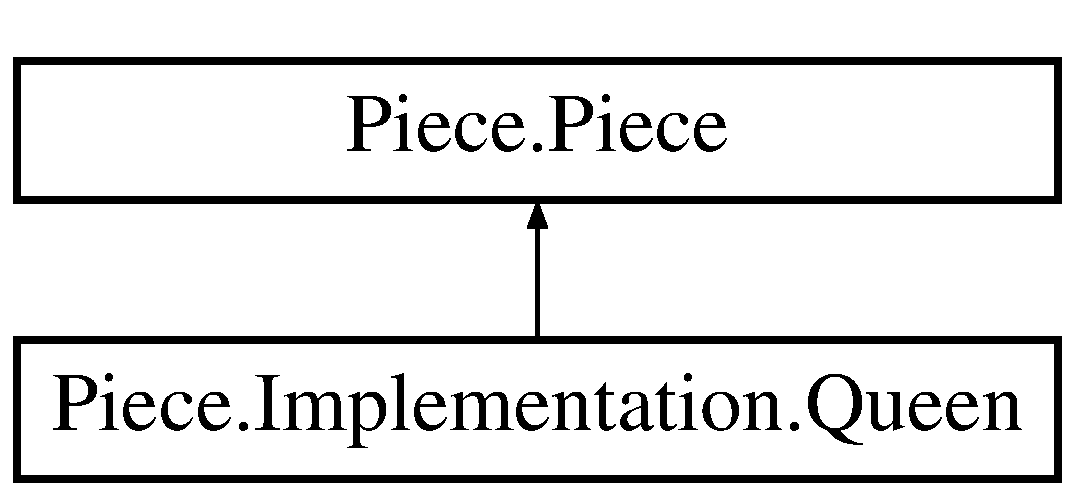
\includegraphics[height=2.000000cm]{classPiece_1_1Implementation_1_1Queen}
\end{center}
\end{figure}
\subsection*{Public Member Functions}
\begin{DoxyCompactItemize}
\item 
\hyperlink{classPiece_1_1Implementation_1_1Queen_a848b7ed8f769c62546d8b8445b30dd16}{Queen} (\hyperlink{classUtil_1_1Position}{Position} start\-Position, int assign\-User\-Id, int assign\-Piece\-Id)  throws Exception 
\end{DoxyCompactItemize}
\subsection*{Protected Member Functions}
\begin{DoxyCompactItemize}
\item 
void \hyperlink{classPiece_1_1Implementation_1_1Queen_a0f7958e2d7f880df8f012b814dd83329}{init\-Directions} ()  throws Exception 
\end{DoxyCompactItemize}
\subsection*{Additional Inherited Members}


\subsection{Detailed Description}
Class that defines the \hyperlink{classPiece_1_1Implementation_1_1Queen}{Queen} chess piece \begin{DoxyAuthor}{Author}
Taccio Yamamoto 
\end{DoxyAuthor}


\subsection{Constructor \& Destructor Documentation}
\hypertarget{classPiece_1_1Implementation_1_1Queen_a848b7ed8f769c62546d8b8445b30dd16}{\index{Piece\-::\-Implementation\-::\-Queen@{Piece\-::\-Implementation\-::\-Queen}!Queen@{Queen}}
\index{Queen@{Queen}!Piece::Implementation::Queen@{Piece\-::\-Implementation\-::\-Queen}}
\subsubsection[{Queen}]{\setlength{\rightskip}{0pt plus 5cm}Piece.\-Implementation.\-Queen.\-Queen (
\begin{DoxyParamCaption}
\item[{{\bf Position}}]{start\-Position, }
\item[{int}]{assign\-User\-Id, }
\item[{int}]{assign\-Piece\-Id}
\end{DoxyParamCaption}
)  throws Exception \hspace{0.3cm}{\ttfamily [inline]}}}\label{classPiece_1_1Implementation_1_1Queen_a848b7ed8f769c62546d8b8445b30dd16}
Constructor 
\begin{DoxyParams}{Parameters}
{\em start\-Position} & -\/ start position of the piece \\
\hline
{\em assign\-User\-Id} & -\/ user identification of the owner of the piece \\
\hline
{\em assign\-Piece\-Id} & -\/ unique id assigned to the piece \\
\hline
\end{DoxyParams}

\begin{DoxyExceptions}{Exceptions}
{\em Exception} & throws possible exceptions from the init\-Directions function \\
\hline
\end{DoxyExceptions}


\subsection{Member Function Documentation}
\hypertarget{classPiece_1_1Implementation_1_1Queen_a0f7958e2d7f880df8f012b814dd83329}{\index{Piece\-::\-Implementation\-::\-Queen@{Piece\-::\-Implementation\-::\-Queen}!init\-Directions@{init\-Directions}}
\index{init\-Directions@{init\-Directions}!Piece::Implementation::Queen@{Piece\-::\-Implementation\-::\-Queen}}
\subsubsection[{init\-Directions}]{\setlength{\rightskip}{0pt plus 5cm}void Piece.\-Implementation.\-Queen.\-init\-Directions (
\begin{DoxyParamCaption}
{}
\end{DoxyParamCaption}
)  throws Exception \hspace{0.3cm}{\ttfamily [inline]}, {\ttfamily [protected]}, {\ttfamily [virtual]}}}\label{classPiece_1_1Implementation_1_1Queen_a0f7958e2d7f880df8f012b814dd83329}
Initializes the legal directions of the piece 
\begin{DoxyExceptions}{Exceptions}
{\em Exception} & throws exceptions from the Direction constructor \\
\hline
\end{DoxyExceptions}


Implements \hyperlink{classPiece_1_1Piece_af8bf9c4edb5bd73c91f3f8b21793ca5b}{Piece.\-Piece}.



The documentation for this class was generated from the following file\-:\begin{DoxyCompactItemize}
\item 
src/\-Piece/\-Implementation/Queen.\-java\end{DoxyCompactItemize}

\hypertarget{classPiece_1_1Implementation_1_1QueenTest}{\section{Piece.\-Implementation.\-Queen\-Test Class Reference}
\label{classPiece_1_1Implementation_1_1QueenTest}\index{Piece.\-Implementation.\-Queen\-Test@{Piece.\-Implementation.\-Queen\-Test}}
}
\subsection*{Public Member Functions}
\begin{DoxyCompactItemize}
\item 
void \hyperlink{classPiece_1_1Implementation_1_1QueenTest_a4e50555387a095381997b0b0a934a63c}{set\-Up} ()  throws Exception 
\item 
\hypertarget{classPiece_1_1Implementation_1_1QueenTest_a5bf74411f11cdce09fed350cbb154de2}{void {\bfseries test\-Piece\-Type} ()}\label{classPiece_1_1Implementation_1_1QueenTest_a5bf74411f11cdce09fed350cbb154de2}

\item 
\hypertarget{classPiece_1_1Implementation_1_1QueenTest_aadc31e79348fef659b3a552e2fc0f69b}{void {\bfseries test\-Can\-Move} ()  throws Exception}\label{classPiece_1_1Implementation_1_1QueenTest_aadc31e79348fef659b3a552e2fc0f69b}

\item 
\hypertarget{classPiece_1_1Implementation_1_1QueenTest_a109a1fb2bdd9f8331a1454023c78be8e}{void {\bfseries test\-Move} ()  throws Exception}\label{classPiece_1_1Implementation_1_1QueenTest_a109a1fb2bdd9f8331a1454023c78be8e}

\item 
\hypertarget{classPiece_1_1Implementation_1_1QueenTest_a1e0211b4b1b204b458bc439bf2de1ebf}{void {\bfseries test\-Get\-Functions} ()}\label{classPiece_1_1Implementation_1_1QueenTest_a1e0211b4b1b204b458bc439bf2de1ebf}

\end{DoxyCompactItemize}


\subsection{Detailed Description}
Created by taccio on 2/13/17. 

\subsection{Member Function Documentation}
\hypertarget{classPiece_1_1Implementation_1_1QueenTest_a4e50555387a095381997b0b0a934a63c}{\index{Piece\-::\-Implementation\-::\-Queen\-Test@{Piece\-::\-Implementation\-::\-Queen\-Test}!set\-Up@{set\-Up}}
\index{set\-Up@{set\-Up}!Piece::Implementation::QueenTest@{Piece\-::\-Implementation\-::\-Queen\-Test}}
\subsubsection[{set\-Up}]{\setlength{\rightskip}{0pt plus 5cm}void Piece.\-Implementation.\-Queen\-Test.\-set\-Up (
\begin{DoxyParamCaption}
{}
\end{DoxyParamCaption}
)  throws Exception \hspace{0.3cm}{\ttfamily [inline]}}}\label{classPiece_1_1Implementation_1_1QueenTest_a4e50555387a095381997b0b0a934a63c}
Calls setup function before every test function 
\begin{DoxyExceptions}{Exceptions}
{\em Exception} & \\
\hline
\end{DoxyExceptions}


The documentation for this class was generated from the following file\-:\begin{DoxyCompactItemize}
\item 
test/\-Piece/\-Implementation/Queen\-Test.\-java\end{DoxyCompactItemize}

\hypertarget{classPiece_1_1Implementation_1_1Rook}{\section{Piece.\-Implementation.\-Rook Class Reference}
\label{classPiece_1_1Implementation_1_1Rook}\index{Piece.\-Implementation.\-Rook@{Piece.\-Implementation.\-Rook}}
}
Inheritance diagram for Piece.\-Implementation.\-Rook\-:\begin{figure}[H]
\begin{center}
\leavevmode
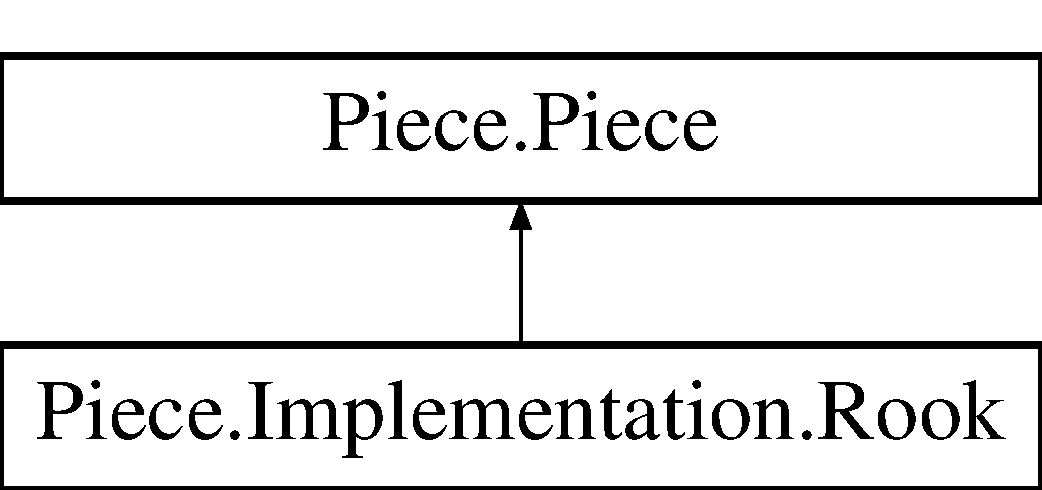
\includegraphics[height=2.000000cm]{classPiece_1_1Implementation_1_1Rook}
\end{center}
\end{figure}
\subsection*{Public Member Functions}
\begin{DoxyCompactItemize}
\item 
\hyperlink{classPiece_1_1Implementation_1_1Rook_a6d1df9c5b8b533c2591225a9e36b1292}{Rook} (\hyperlink{classUtil_1_1Position}{Position} start\-Position, int assign\-User\-Id, int assign\-Piece\-Id)  throws Exception
\end{DoxyCompactItemize}
\subsection*{Protected Member Functions}
\begin{DoxyCompactItemize}
\item 
void \hyperlink{classPiece_1_1Implementation_1_1Rook_a0288b5ea743dcb4286fb0c91bd163f0d}{init\-Directions} ()  throws Exception
\end{DoxyCompactItemize}
\subsection*{Additional Inherited Members}


\subsection{Detailed Description}
Class that defines the \hyperlink{classPiece_1_1Implementation_1_1Rook}{Rook} chess piece \begin{DoxyAuthor}{Author}
Taccio Yamamoto 
\end{DoxyAuthor}


\subsection{Constructor \& Destructor Documentation}
\hypertarget{classPiece_1_1Implementation_1_1Rook_a6d1df9c5b8b533c2591225a9e36b1292}{\index{Piece\-::\-Implementation\-::\-Rook@{Piece\-::\-Implementation\-::\-Rook}!Rook@{Rook}}
\index{Rook@{Rook}!Piece::Implementation::Rook@{Piece\-::\-Implementation\-::\-Rook}}
\subsubsection[{Rook}]{\setlength{\rightskip}{0pt plus 5cm}Piece.\-Implementation.\-Rook.\-Rook (
\begin{DoxyParamCaption}
\item[{{\bf Position}}]{start\-Position, }
\item[{int}]{assign\-User\-Id, }
\item[{int}]{assign\-Piece\-Id}
\end{DoxyParamCaption}
)  throws Exception\hspace{0.3cm}{\ttfamily [inline]}}}\label{classPiece_1_1Implementation_1_1Rook_a6d1df9c5b8b533c2591225a9e36b1292}
Constructor 
\begin{DoxyParams}{Parameters}
{\em start\-Position} & -\/ start position of the piece \\
\hline
{\em assign\-User\-Id} & -\/ user identification of the owner of the piece \\
\hline
{\em assign\-Piece\-Id} & -\/ unique id assigned to the piece \\
\hline
\end{DoxyParams}

\begin{DoxyExceptions}{Exceptions}
{\em Exception} & throws possible exceptions from the init\-Directions function \\
\hline
\end{DoxyExceptions}


\subsection{Member Function Documentation}
\hypertarget{classPiece_1_1Implementation_1_1Rook_a0288b5ea743dcb4286fb0c91bd163f0d}{\index{Piece\-::\-Implementation\-::\-Rook@{Piece\-::\-Implementation\-::\-Rook}!init\-Directions@{init\-Directions}}
\index{init\-Directions@{init\-Directions}!Piece::Implementation::Rook@{Piece\-::\-Implementation\-::\-Rook}}
\subsubsection[{init\-Directions}]{\setlength{\rightskip}{0pt plus 5cm}void Piece.\-Implementation.\-Rook.\-init\-Directions (
\begin{DoxyParamCaption}
{}
\end{DoxyParamCaption}
)  throws Exception\hspace{0.3cm}{\ttfamily [inline]}, {\ttfamily [protected]}, {\ttfamily [virtual]}}}\label{classPiece_1_1Implementation_1_1Rook_a0288b5ea743dcb4286fb0c91bd163f0d}
Initializes the legal directions of the piece 
\begin{DoxyExceptions}{Exceptions}
{\em Exception} & throws exceptions from the Direction constructor \\
\hline
\end{DoxyExceptions}


Implements \hyperlink{classPiece_1_1Piece_af8bf9c4edb5bd73c91f3f8b21793ca5b}{Piece.\-Piece}.



The documentation for this class was generated from the following file\-:\begin{DoxyCompactItemize}
\item 
src/\-Piece/\-Implementation/Rook.\-java\end{DoxyCompactItemize}

\hypertarget{classPiece_1_1Implementation_1_1RookTest}{\section{Piece.\-Implementation.\-Rook\-Test Class Reference}
\label{classPiece_1_1Implementation_1_1RookTest}\index{Piece.\-Implementation.\-Rook\-Test@{Piece.\-Implementation.\-Rook\-Test}}
}
\subsection*{Public Member Functions}
\begin{DoxyCompactItemize}
\item 
void \hyperlink{classPiece_1_1Implementation_1_1RookTest_a52c69be339c067d204111f0c5b8a4d1f}{set\-Up} ()  throws Exception 
\item 
void \hyperlink{classPiece_1_1Implementation_1_1RookTest_aeb9a754f956f53d03428f3638b20e6de}{test\-Piece\-Type} ()
\item 
void \hyperlink{classPiece_1_1Implementation_1_1RookTest_a8569a78cd2e7cb7d80b4c2d96a88107e}{test\-Can\-Move} ()  throws Exception
\item 
void \hyperlink{classPiece_1_1Implementation_1_1RookTest_a52065b5c7466bdbff9ec46a61d528ee3}{test\-Move} ()  throws Exception
\item 
void \hyperlink{classPiece_1_1Implementation_1_1RookTest_a99f03e51fac8ac25adec7c5c3044f1bf}{test\-Get\-Functions} ()
\end{DoxyCompactItemize}


\subsection{Detailed Description}
Created by taccio on 2/13/17. 

\subsection{Member Function Documentation}
\hypertarget{classPiece_1_1Implementation_1_1RookTest_a52c69be339c067d204111f0c5b8a4d1f}{\index{Piece\-::\-Implementation\-::\-Rook\-Test@{Piece\-::\-Implementation\-::\-Rook\-Test}!set\-Up@{set\-Up}}
\index{set\-Up@{set\-Up}!Piece::Implementation::RookTest@{Piece\-::\-Implementation\-::\-Rook\-Test}}
\subsubsection[{set\-Up}]{\setlength{\rightskip}{0pt plus 5cm}void Piece.\-Implementation.\-Rook\-Test.\-set\-Up (
\begin{DoxyParamCaption}
{}
\end{DoxyParamCaption}
)  throws Exception \hspace{0.3cm}{\ttfamily [inline]}}}\label{classPiece_1_1Implementation_1_1RookTest_a52c69be339c067d204111f0c5b8a4d1f}
Calls setup function before every test function 
\begin{DoxyExceptions}{Exceptions}
{\em Exception} & \\
\hline
\end{DoxyExceptions}
\hypertarget{classPiece_1_1Implementation_1_1RookTest_a8569a78cd2e7cb7d80b4c2d96a88107e}{\index{Piece\-::\-Implementation\-::\-Rook\-Test@{Piece\-::\-Implementation\-::\-Rook\-Test}!test\-Can\-Move@{test\-Can\-Move}}
\index{test\-Can\-Move@{test\-Can\-Move}!Piece::Implementation::RookTest@{Piece\-::\-Implementation\-::\-Rook\-Test}}
\subsubsection[{test\-Can\-Move}]{\setlength{\rightskip}{0pt plus 5cm}void Piece.\-Implementation.\-Rook\-Test.\-test\-Can\-Move (
\begin{DoxyParamCaption}
{}
\end{DoxyParamCaption}
)  throws Exception\hspace{0.3cm}{\ttfamily [inline]}}}\label{classPiece_1_1Implementation_1_1RookTest_a8569a78cd2e7cb7d80b4c2d96a88107e}
Tests the can\-Move() function 
\begin{DoxyExceptions}{Exceptions}
{\em Exception} & throws Exception from can\-Move() funciton \\
\hline
\end{DoxyExceptions}
\hypertarget{classPiece_1_1Implementation_1_1RookTest_a99f03e51fac8ac25adec7c5c3044f1bf}{\index{Piece\-::\-Implementation\-::\-Rook\-Test@{Piece\-::\-Implementation\-::\-Rook\-Test}!test\-Get\-Functions@{test\-Get\-Functions}}
\index{test\-Get\-Functions@{test\-Get\-Functions}!Piece::Implementation::RookTest@{Piece\-::\-Implementation\-::\-Rook\-Test}}
\subsubsection[{test\-Get\-Functions}]{\setlength{\rightskip}{0pt plus 5cm}void Piece.\-Implementation.\-Rook\-Test.\-test\-Get\-Functions (
\begin{DoxyParamCaption}
{}
\end{DoxyParamCaption}
)\hspace{0.3cm}{\ttfamily [inline]}}}\label{classPiece_1_1Implementation_1_1RookTest_a99f03e51fac8ac25adec7c5c3044f1bf}
Tests different Get funcitons \hypertarget{classPiece_1_1Implementation_1_1RookTest_a52065b5c7466bdbff9ec46a61d528ee3}{\index{Piece\-::\-Implementation\-::\-Rook\-Test@{Piece\-::\-Implementation\-::\-Rook\-Test}!test\-Move@{test\-Move}}
\index{test\-Move@{test\-Move}!Piece::Implementation::RookTest@{Piece\-::\-Implementation\-::\-Rook\-Test}}
\subsubsection[{test\-Move}]{\setlength{\rightskip}{0pt plus 5cm}void Piece.\-Implementation.\-Rook\-Test.\-test\-Move (
\begin{DoxyParamCaption}
{}
\end{DoxyParamCaption}
)  throws Exception\hspace{0.3cm}{\ttfamily [inline]}}}\label{classPiece_1_1Implementation_1_1RookTest_a52065b5c7466bdbff9ec46a61d528ee3}
Tests the move() function 
\begin{DoxyExceptions}{Exceptions}
{\em Exception} & throws Exception from move() funciton \\
\hline
\end{DoxyExceptions}
\hypertarget{classPiece_1_1Implementation_1_1RookTest_aeb9a754f956f53d03428f3638b20e6de}{\index{Piece\-::\-Implementation\-::\-Rook\-Test@{Piece\-::\-Implementation\-::\-Rook\-Test}!test\-Piece\-Type@{test\-Piece\-Type}}
\index{test\-Piece\-Type@{test\-Piece\-Type}!Piece::Implementation::RookTest@{Piece\-::\-Implementation\-::\-Rook\-Test}}
\subsubsection[{test\-Piece\-Type}]{\setlength{\rightskip}{0pt plus 5cm}void Piece.\-Implementation.\-Rook\-Test.\-test\-Piece\-Type (
\begin{DoxyParamCaption}
{}
\end{DoxyParamCaption}
)\hspace{0.3cm}{\ttfamily [inline]}}}\label{classPiece_1_1Implementation_1_1RookTest_aeb9a754f956f53d03428f3638b20e6de}
Checks the piece has correct \hyperlink{enumPiece_1_1PieceType}{Piece\-Type} 

The documentation for this class was generated from the following file\-:\begin{DoxyCompactItemize}
\item 
test/\-Piece/\-Implementation/Rook\-Test.\-java\end{DoxyCompactItemize}

\hypertarget{classGame_1_1User}{\section{Game.\-User Class Reference}
\label{classGame_1_1User}\index{Game.\-User@{Game.\-User}}
}


\subsection{Detailed Description}
Created by taccio on 2/13/17. 

The documentation for this class was generated from the following file\-:\begin{DoxyCompactItemize}
\item 
src/\-Game/User.\-java\end{DoxyCompactItemize}

\hypertarget{classUserInterface_1_1UserInterface}{\section{User\-Interface.\-User\-Interface Class Reference}
\label{classUserInterface_1_1UserInterface}\index{User\-Interface.\-User\-Interface@{User\-Interface.\-User\-Interface}}
}


\subsection{Detailed Description}
Created by taccio on 2/13/17. 

The documentation for this class was generated from the following file\-:\begin{DoxyCompactItemize}
\item 
src/\-User\-Interface/User\-Interface.\-java\end{DoxyCompactItemize}

\addcontentsline{toc}{part}{Index}
\printindex
\end{document}
